
\documentclass[12pt, a4paper]{article}
\usepackage{geometry}
\usepackage{setspace}
\usepackage{lipsum}
\usepackage{graphicx}
\usepackage{caption}
\usepackage{lineno}
\usepackage{apacite}
\usepackage{natbib}
\usepackage{xcolor}
\usepackage{amsmath}
\usepackage{booktabs}
\usepackage{multirow}
\usepackage{pdflscape}
\usepackage{float}
\usepackage{array}
\usepackage{amsmath}
\usepackage{amsfonts}
\usepackage{siunitx}
\usepackage{dcolumn}
\usepackage{booktabs}
\usepackage{tabularx}
\usepackage{tocloft}
\usepackage{sectsty}
\usepackage{apacite}
\usepackage{makecell}
\geometry{a4paper, left=3cm, right=3cm, top=2.5cm, bottom=2.5cm}
\graphicspath{{figures/}}
\captionsetup[figure]{skip=4pt}
\captionsetup[table]{skip=4pt}
\newcolumntype{Y}{S[table-format=5.2(5)]}
% Remove table numbers from the list of tables
\makeatletter
\renewcommand{\cfttabpresnum}{\begin{lrbox}{\@tempboxa}}
	\renewcommand{\cfttabaftersnum}{\end{lrbox}}
\makeatother
% Remove table numbers from the list of tables
\makeatletter
\renewcommand{\cftfigpresnum}{\begin{lrbox}{\@tempboxa}} % Remove figure numbers from the list of figures
	\renewcommand{\cftfigaftersnum}{\end{lrbox}}
\makeatother
\sectionfont{\small}
\subsectionfont{\small}
\subsubsectionfont{\small}
\begin{document}
\newpage % Start content on a new page
	\begin{center}
		\large{Household Vulnerability And Environmental Dependence in Rural Nepal \\ \vspace{0.8cm} \\
		\fontsize{13}{15}\selectfont Sanjeev Nhemhafuki\textsuperscript{$\dag$}, Bipin Khadka\textsuperscript{$\dag$}, \\ Resham Thapa - Parajuli\textsuperscript{$\ddag$}
	\end{center} 
\begin{center}
\section*{\large{Abstract}}
\end{center}	

\addcontentsline{toc}{section}{\MakeUppercase{Abstract}}
\renewcommand{\thepage}{\roman{page}}
\setcounter{page}{5}
\setstretch{1.5}
this paper examines whether the households dependent on environmental income are vulnerable in rural setting of three distinct geographic region of Nepal. For this purpose, the study develops a composite household vulnerability index based on the various capitals owned by the households and relates the latter with the share of environmental income to total income. The study uses the environmental augmented household-level livelihood longitudinal data-set of Nepal, known as PEN (Poverty Environment Network) dateset. It covers the period of 2006, 2009 and 2012. Further, we assess the relationship between the household vulnerability and environmental dependence. The results suggest that Environmental dependence and Household Vulnerability are positively associated. The level of vulnerability is heterogeneous in different ecological zone. Mountainous region seems more vulnerable as compared to Lowland and Mid-hill region. Rural households are confined to rural activities which are related to environment. Therefore, more environmental dependence has to do with more vulnerability. This provides critical evidence for a policy debate within society, which argues for the global implementation of Community Forest Management and Conservation Area Management.   \\

\hspace{-0.6cm}\textbf{Keywords:} Vulnerability, Environmental Depenedence, Spatial Panel Data\\
\\
\hspace{-0.6cm}\textbf{JEL Classification:} Q00, Q50, Q56 

\renewcommand{\thefootnote}{\fnsymbol{footnote}}
\footnotetext[2]{$\dag$ Graduate student \ \ - Central Department of Econmics, Tribhuvan University}
\footnotetext[3]{$\ddag$ Associate Professor - Central Department of Economics, Tribhuvan University}
\clearpage % Start content on a new page
\begin{center}
\section*{\large{CHAPTER I \\ \vspace{-0.3cm} INTRODUCTION}}
\end{center}
\addcontentsline{toc}{section}{\textbf{CHAPTER I:  INTRODUCTION}}
\renewcommand{\thepage}{\arabic{page}} 
\setcounter{page}{1}
This chapter presents the study’s background, statement of the problem,
research question, and thesis objectives. In addition, it highlights the significance
and limitations of the study.\\
\subsection*{1.1 Background of the Study}
\addcontentsline{toc}{subsection}{1.1 Background of the Study}
\renewcommand{\thepage}{\arabic{page}} 
\ \ \ According to The World \cite{world2018rural} the global rural population constituted 43.5\% 
of the global population. The prevailing trend indicates a decline in the rural population is declining attributed to social, economic, technological, infrastructure, and environmental influences as discussed by \citep{jaszczak2018phenomenon}. The \cite{UNDP} projects that by 2050, sixty-eight percent of the world’s population will be urban by 2050.
While scholars and institutions project a decline in the share of the rural population, the number of people living in rural areas still remains significant.

The population residing in rural areas faces considerable vulnerability, as highlighted by \cite{acharya2008dimension}. The global rural population is estimated to be 3.4 billion, according to \cite{Worldbank2022}. In terms of poverty, a striking 80 percent of those living in extreme poverty are found in rural areas \citep{world2021state}. Additionally, the escalating risks of climate change disproportionately affect rural populations \citep{Researchoverview2022}, posing a significant threat to their livelihoods, especially given the heavy dependence of many rural households on the natural environment. This phenomenon poses a massive threat to the poor rural livelihoods \citep{pelser2022climate}. \cite{angelsen2014environmental} contends that the natural environment such as forests and other natural areas, are crucial for sustaining rural livelihoods. So environmental reasons, along with political and economic, stands amongst the drivers of migration \citep{mcnamara2016insecure}.

The rural population is increasingly falling into poverty, and those left behind are becoming more challenging to reach \citep{UN2019}. This trend has contributed to a rise in migration from rural areas \citep{lazarte2017understanding}. In some instances, migrants are unfairly blamed for urban poverty \citep{tacoli2015rural}. Consequently, this imbalance in rural-urban resource distribution results in the mismanagement of opportunities and resources in rural areas. Simultaneously, it fuels heightened competition for urban resources, leading to their scarcity \citep{artuso2011state}. 

Against this backdrop, it becomes imperative to investigate rural areas, their inhabitants, and their means of sustaining themselves to develop a more comprehensive understanding of rural economies. The residents of these areas predominantly rely on their surrounding environment, with natural resources assuming a pivotal role in their livelihoods \citep{nawrotzki2012natural}. Frequently, income generated from nature serves as a crucial safety net during periods of deficiencies in other livelihood activities, supporting immediate consumption needs and offering a potential pathway out of poverty \citep{angelsen2003exploring}. However, relying on environment also may contribute to the vulnerability of the households. Therefore, a thorough examination of the sources of livelihood in rural regions and the extent to which households are reliant on the environment becomes crucial.
 
 The most frequently employed frameworks for rural livelihood and vulnerability analysis are \cite{anani1999sustainable}, \cite{dfid1999sustainable}, and \cite{ellis1999rural}. These frameworks serve as foundational tools for scrutinizing rural households within specific contexts and their livelihood resources. The Sustainable Livelihood Approach, incorporating key elements such as livelihood resources, vulnerability contexts, institutional processes, livelihood strategies, and outcomes, provides a comprehensive structure for rural livelihood analysis \citep{walelign2017dynamics}. Numerous studies have utilized frameworks like the Sustainable Livelihood Framework, Livelihood Assets Framework, Vulnerability Framework, and others to conduct in-depth analyses.

\cite{nawrotzki2012natural} underscores the central importance of natural resources in rural livelihoods through a thorough analysis. Building on this, \cite{diaz2019livelihood} establishes that capital assets play a crucial role in determining the livelihood strategies adopted by small-scale farmers. In addressing poverty in rural areas, \cite{mukotami2014rural} advocates for the promotion of non-farm activities, emphasizing that the poorest rural groups face limited opportunities for diversification, hindering the accumulation of resources for investment purposes. Furthermore, \cite{cavendish2008poverty}, in exploring the link between environmental income and inequality, identifies access to non-environmental cash income as the most significant contributor to rural inequality.

\cite{charlery2015assessing} employs a decomposition method to distinguish between stochastic and structural poverty within households, utilizing both income data and assets index. The study reveals that those classified as income poor exhibit a higher dependence on environmental resources in rural Nepal. In a related vein, \cite{walelign2017dynamics} employs clustering to identify various remunerative strategy groups, highlighting a higher reliance on environmental resources within the cluster employing the least remunerative strategies. The author suggests, based on this finding, that Nepalese rural households in an upward transition phase show a reduction in environmental dependency, emphasizing the importance of enhancing poverty reduction strategies. 

In the study conducted by \cite{walelign2020environmental}, it is observed that rural Nepalese households with high reliance on environmental resources exhibit lower income and asset endowments. Conversely, households with lower environmental reliance fare better in terms of both income and assets. Adding to this perspective, \cite{walelign2021poverty} highlights the impact of poor infrastructures in mountainous areas of Nepal, resulting in households having fewer assets and lower income compared to their counterparts in mid-hills and lowlands. Furthermore, \cite{chhetri2022importance} concludes that forest and environmental income remain the primary source of income and livelihoods for poor and marginalized households in Nepal, with a notable decrease in forest and environmental incomes as household income increases.

A substantial body of scholarly literature, spanning both international and national contexts, has delved into the exploration of factors influencing the livelihood strategies adopted by rural households across diverse countries. For instance, \cite{angelsen2014environmental} scrutinizes the determinants of household income across 8,000 households in 24 developing nations. The econometric model employed in the analysis incorporates factors such as household characteristics, assets, shocks, institutions, location, and site-level economic factors. In a related study, \cite{emeru2022determinants} identifies determinants of livelihood diversification strategies, including the age of the household, education status, family size, access to credit, market access, and positive impacts from training and extension services. Similarly, \cite{amevenku2019determinants} underscores the significance of marital status of the household head, the duration of food shortages experienced per year, access to credit and extension services, distance to regular markets and district capitals, as well as experience in fishery, as major determinants influencing livelihood strategies.

In the specific context of rural Nepal, there is a noticeable scarcity of literature assessment of the household vulnerability and environmental dependence. Furthermore, a critical gap exists in the identification and analysis of households that are vulnerable which is a crucial step to help policymakers foresee prospective routes for different segments, and thus frame out interventions more effectively. To address these gaps, this study endeavors to provide a comprehensive analysis, aiming to contribute valuable insights and enhance our understanding household vulnerability and its relationship with the environmental dependence in the rural landscapes of Nepal.

\subsection*{1.2 Statement of the Problem }
\addcontentsline{toc}{subsection}{1.2 Statement of the Problem }
\renewcommand{\thepage}{\arabic{page}}
Developing countries are often characterized having majority of rural population. Many communities in developing countries heavily rely on natural resources and the environment for their rural livelihood strategies \citep{adger2000social, ahmadpour2020factors, chambers1992sustainable, ellis1999rural}. However, past literature has not thoroughly studied environmental dependency and its influence on household vulnerability. This could hinder the provision of a more accurate representation of environmental dependency, potentially limiting our understanding of the true impact of environmental changes on rural household vulnerability. Consequently, this gap in the literature may impede the development of effective policies to mitigate these effects.

Moreover, although \citep{mao2020rural, shan2020determinants, lorato2019determinants} have conducted some analysis on the determinants of rural livelihood strategies, there is a compelling need for more in-depth examination to gain a comprehensive understanding of the relationship with household vulnerability of these strategies, particularly those related with environment and nature. This entails a thorough investigation into the social, economic, and environmental factors that shape the decisions and choices of rural households and communities. Such a nuanced analysis is crucial for developing a holistic perspective on the intricate dynamics that influence policy and decision making.

In summary, the absence of a comprehensive understanding of environmental dependency and the household vulnerability determinants presents a substantial challenge to sustainable development and poverty reduction efforts in numerous rural areas in Nepal. It is essential to study the environmental dependency, particularly in the context of rapidly changing climatic environment and its influence on livelihoods and vulnerability. Further, there is a very limited studies that have assessed the transition of households to new state from old state of vulnerability. The panel structure of the dateset allows this study to assess the time-varying vulnerability transition from one state to another and assess how have the factors played role in the transience and persistence. It is imperative to address these knowledge gaps to formulate effective policies and interventions that can support rural communities and enhance their resilience in response to environmental changes. This proactive approach is essential for fostering sustainable development and improving the well-being of rural populations.

\subsection*{1.3 Research Questions}
\addcontentsline{toc}{subsection}{1.3 Research Questions }
\renewcommand{\thepage}{\arabic{page}}
The research question centers around the necessity for a more comprehensive understanding of the vulnerability of impoverished rural households and the factors influencing it. Notably, there is a gap in the assessment of household vulnerability based on the various components that contribute to the household's vulnerability, restricting a nuanced comprehension of the actual impact of the factors. Further, there is a gap of studies which studies the vulnerability positions of the households relative to the earlier positions. Moreover, a deeper analysis is warranted to scrutinize the social, economic, and environmental factors shaping the decisions of rural households and communities. Addressing these knowledge gaps is pivotal for developing policies and interventions that foster the resilience of rural communities in the face of environmental change, thereby supporting sustainable development and poverty reduction efforts in rural areas.
\vspace{1cm}
\newline
\textbf{Research Questions:} 
\begin{enumerate}
	\item[(i)] \parbox[t]{\linewidth}{What are the differences in household vulnerability to shocks and crisis across households in rural Nepal?}
	\item [(ii)] \parbox[t]{\linewidth}{What are the factors that play a role in determining the vulnerability to shocks and crisis of rural households in Nepal?}
\end{enumerate}
\subsection*{1.4 Objectives of the Study }
\addcontentsline{toc}{subsection}{1.4 Objectives of the Study   }
\renewcommand{\thepage}{\arabic{page}}
\textbf{General Objectives}
\\
The study aims to assess the household vulnerability to shocks and crisis and its determinants of the households in rural Nepal. To achieve the objective, two broad objectives has been set:
\begin{enumerate}
	\item[(i)] \parbox[t]{\linewidth}{Provide an overview of rural household vulnerability across households.}
	\item [(ii)] \parbox[t]{\linewidth}{Determine the factors that affect the household vulnerability with a focus on rural household's reliance on environmental resources.}
\end{enumerate}
\vspace{1cm}

\textbf{Specific Objectives} 
\\
To achieve the broad objective, two specific objective has been set:
\begin{enumerate}
	\item[(i)] \parbox[t]{\linewidth}{Compare the extent of rural household vulnerability to shocks and crisis within and across the households in selected villages from rural Nepal. Analyze the differences in the degree of vulnerability among these strategies.}

 	\item[(ii)] \parbox[t]{\linewidth}{Identify and analyze the primary determinants influencing the rural household vulnerability to shocks and crisis in Nepal, with a particular emphasis on the environmental reliance.} 
 \end{enumerate}  \\ \vspace{0.5cm}

\subsection*{1.5 Significance of the Study}
\addcontentsline{toc}{subsection}{1.5 Significance of the Study}
\renewcommand{\thepage}{\arabic{page}}
In the realm of environmental dependency across household strategy categories, the agricultural environment-based strategy group demonstrates the highest levels for both poverty incidence and environmental dependency, as noted by \cite{walelign2016livelihood}. Despite this, there is a notable dearth of research on how this dependence could be a factor that contribute to vulnerability in rural communities within the context of Nepal. Furthermore, no study has specifically addressed the relationship between the household vulnerability and environmental dependence.
The present study capitalizes on the panel characteristics of the data set. By utilizing established econometric tools, this thesis aims to fulfill its objectives. The findings of this study are anticipated to provide insights into the nature and differences of household vulnerability and environmental reliance in Nepal's rural communities. This information holds significance for policymakers as they assess which policies to prioritize in efforts to enhance the well-being of rural communities.

\subsection*{1.6 Scope and Limitations of the Study}
\addcontentsline{toc}{subsection}{1.6 Scope and Limitations of the Study}
\renewcommand{\thepage}{\arabic{page}}
\textbf{Scope:}\\
This study aims to examine the determinants of rural household vulnerability based on various assets of the hosueholds in the Chitwan (lowlands), Kaski (mid-hills), and Mustang (mountains)
of Nepal. The study will use a 3-wave panel data set collected in 2006, 2009, and 
2012, and will analyze the relationships between household demographics, assets, 
income, and their impact on rural household vulnerability. \\

The study investigates the array of assets available to households within the research area, encompassing financial, physical, social, and human resources. It delves into the variability of households' vulnerability compared to others, considering factors such as income, education, access to services, and social networks. Key determinants of household vulnerability are identified, including economic status, environmental conditions, health, and social capital. Furthermore, the study examines how these determinants fluctuate across diverse regions and evolve over time, providing insights into the dynamic nature of vulnerability within different contexts.
This study aims at assessing the household vulnerability and environmental dependence of the rural households in Nepal.\\
\newline
\textbf{Limitations:}
\begin{enumerate}
	\item[(i)] \parbox[t]{\linewidth}{The study is limited to three districts in Nepal and may not be representative of 
	other regions or countries.}
	\item[(ii)] \parbox[t]{\linewidth}{The analysis will rely on secondary data.}
	\item[(iii)] \parbox[t]{\linewidth}{The study will focus on a limited set of variables and may  and may leave out consideration of other equally important factors that affect the household vulnerability.}\\
\end{enumerate}

\subsection*{1.7 Organizations of the Study}
\addcontentsline{toc}{subsection}{1.7 Organizations of the Study}
\renewcommand{\thepage}{\arabic{page}}
The following chapter provides an overview of the literature, encompassing
theoretical and empirical reviews and addressing the existing research gaps. Moving on to Chapter 3, the research plan is delved into, encompassing aspects such as research design, philosophical considerations, variable operationalization, conceptual framework, empirical model, and data sources. Likewise, Chapter Four is dedicated to the presentation of data analysis and subsequent discussions. Concluding
the report, the final chapter outlines the conclusions drawn, recommendations, and
potential avenues for future extensions.

\clearpage

\begin{center}
\section*{\large{CHAPTER II \\ \vspace{-0.3cm} REVIEW OF LITERATURE}}
\end{center}
\addcontentsline{toc}{section}{\textbf{CHAPTER II: REVIEW OF LITERATURE}}
\renewcommand{\thepage}{\arabic{page}}
\setstretch{1.5}
This chapter reviews theoretical and empirical literature, encompassing theoretical
issues and its empirical evidence. The scientific literature available in credible sources
and references is examined. Such as the Journals and Google Scholar.\\
\subsection*{2.1  Theoritical Review}
\addcontentsline{toc}{subsection}{2.1 Introduction}
\renewcommand{\thepage}{\arabic{page}}
\setstretch{1.5}
The main economic theory to study sustainable livelihoods was developed by Robert Chambers and Gordon Conway in mid 1980s. \cite{chambers1992sustainable} contends that a sustainable livelihood is one that can withstand stress and shock, maintain or improve its assets and capabilities, and create opportunities for future generations to live sustainably. It also generates benefits for other livelihoods both locally and globally as well as over the long term. The author created the Sustainable Livelihood Approach (SLA) for the purpose of evaluating various vulnerability contexts to improve the effectiveness of development cooperation. 

Based on the Sustainable Livelihood Approach (SLA), the Sustainable Livelihood Framework (SLF) was proposed with a particular emphasis on the institutional processes which mediate the ability to carry out combination of livelihood strategies with the given livelihood resources in a particular context to achieve an outcome. Some of the well-known livelihood frameworks are those proposed by Department of International Department \cite{dfid1999sustainable}, \cite{ellis1999rural} and \cite{scoones2013livelihoods}. 

\cite{dfid1999sustainable} defines livelihoods broadly and systematically, considering the various assets that individuals or communities can draw upon for sustainable living. It emphasizes the inter-linkage of various capitals (Human, Social, Financial, Physical, and Natural Capital) the households possess with the livelihood outcomes. The framework provides a holistic viewpoint by taking into consideration the dynamic exchange of the capitals and how they influence the result of livelihood. 

\cite{ellis1999rural}  builds on the DFID model by introducing the idea of vulnerability and emphasizes the importance of understanding the factors that makes certain people or groups more vulnerable to shocks and stresses. The author highlights the significance of understanding the elements that make people or communities more vulnerable to shocks and pressures and presents the idea of vulnerability as a major predictor of livelihood strategies and results.

\cite{scoones2013livelihoods} contributed to SLF issue by emphasizing the importance of social relations and political economy in determining the livelihoods. The author's work highlights the need for critical analysis of social relations and political context and how they impact the household's ability to secure more sustainable livelihoods. The framework stress the need for a comprehensive understanding of livelihoods, taking into consideration not only the assets and vulnerability but also the the social, economic and political dimension. 

In a nutshell, DFID framework provides a comprehensive overview of various capitals that impact livelihoods. It acknowledges the concept of vulnerability but doesn't make it a central focus. Also, it does not explicitly delve into social and political dimension of livelihoods. Ellis on the other side of the spectrum, introduces the concept of vulnerability and places a strong emphasis on understanding the elements that increase the likelihood of failure. The framework includes some consideration of political and institutional factors but is centered more on vulnerability. Scoone highlights the critical role of political economy and power structures in shaping the livelihoods. Each framework brings unique perspectives to the understanding of sustainable livelihoods, with varying levels of focus on capitals, vulnerability, political economy, and power dynamics.    
         
\subsection*{2.2 Household Vulnerability}
\addcontentsline{toc}{subsection}{2.2 Household Vulnerability}
\renewcommand{\thepage}{\arabic{page}}
\setstretch{1.5}
Vulnerability is a concept that is applied in various disciplines, including engineering, ecology, economics, psychology and sociology \citep{fang2016rural}. Vulnerability refers to a state in which a person feels insecure when something harmful occurs \citep{chambers2006vulnerability}. "Vulnerable" refers to something that is likely to be harmed or wounded in everyday language. The term "Vulnerable", which means "wound", is dervied from the Latin word "vulnerare," \citep{calvo2005measuring}. On a similar note, \cite{chambers1989editorial}  states that vulnerability “refers to exposure to contingencies and stress, which is defenselessness, meaning a lack of means to cope without damaging loss”. 

The concept of household vulnerability is both controversial and multifaceted \citep{zhang2020capital}. So, household vulnerability analysis requires identification of not only the threat, but also the ‘resilience’, or responsiveness, in exploiting opportunities, and in resisting, or recovering from, the negative consequences of a changing environment \citep{moser1998asset}. In this perspective, \cite{bernier2014resilience} defines the resilience as the ability of a person, household, community, or system to adapt over time to shocks and proactively lower the risk of future shocks is what we refer to as resilience; these efforts promote growth and development as opposed to stability.

Many scholars conceptualise resilience as capacities that are driven by a set of capitals to produce outcomes such as influencing preparedness, mitigating impacts, and enhancing recovery against some risks. \cite{gaisie2021complexity} reveals complex relationship between household capitals and disaster outcomes in Ghana. The study finds that household capitals indicating higher economic status were linked to worse impacts from flooding but were essential for facilitating household recovery over time. \cite{zhang2020capital} in the similar study conducted in China suggests that all forms of capital (financial, human, natural, physical, and social 
capital) of a household were important determinants of household vulnerability. The term "resilience" and "vulnerability" has been used in the literature as antonyms of one another. The basic concept is that the more resilient a system, the less vulnerable it is. 

\cite{fang2016rural}, by constructing a composite vulnerability index, assessed the household vulnerability of the households in Shigatze Prefecture in Tibet
Autonomous Region (TAR) in China. The index has been constructed by taking into account the factors such as food variability, literacy rate of labor force, cash income and expenditure, precipitation vulnerability and drought area. The study finds that the factors under consideration reflects the close relationship between the basic requirement of th rural households in te harsh plataeu environment, less developed regions and vulnerability.    

\cite{antwi2013characterising} assessed the vulnerability to drought across six communities in Ghana. The study reveals varying vulnerability degrees influenced by socioeconomic factors. Authors find that less vulnerable households depict the resilience through alternative livelihoods and social connections. On a similar study, \cite{rahman2023households} quantifies cyclone vulnerability in rural Bangladesh, emphasizing  the multidimensional nature of vulnerability encompassing social, economic, physical, institutional, environmental, and attitudinal factors. The research, focusing on Kalmegha and Patharghata regions, reveals distinct vulnerability patterns, particularly in environmental and composite aspects. \cite{notenbaert2013derivation} constructed the household vulnerability index and explores the vulnerability and coping capacity related to current variability conditions with  focus on the adaptive capacity of the households. The study suggests that distance to paved road, income diversification and savings of the households significantly influences the household vulnerability. 

\subsection*{2.3 Review of National Studies}
\addcontentsline{toc}{subsection}{2.3 Review of National Studies}
\renewcommand{\thepage}{\arabic{page}}
\setstretch{1.5}
Numerous studies have been conducted with respect to the assessment of vulnerability across Nepal. The following study uses the country-level data to investigate the vulnerability. \cite{aksha2019analysis} investigated the social vulnerability in Nepal by adapting Social Vulnerability Index (SoVI) methods to Nepalese context using the full data set of 2011 census provided by the Central Bureau of Statistics (CBS). The study employs the Principal Component Analysis (PCA) to generate the independent set of factors to calculate the SoVI score. The SoVI for Nepal was calculated for each spatial unit (3918 village development committee and 53 municipalities). The components used in the study are renters and occupation, poverty and poor infrastructure, favorable social conditions, migration and gender, ethnicity, medical services, education. The study finds that social vulnerability is particularly high in areas that have concentrations of Dalit and Minority populations.    

\cite{shahiestimating} estimate the vulnerability score for Nepal using a three-stage feasible generalized least square technique to assess vulnerability to poverty. Utilizing the third round of Nepal Living Standards Survey data, the study's findings reveal that Nepal's overall vulnerability is 33 percent, indicating the probability of households falling into poverty due to various shocks such as death, illness, unemployment, and other idiosyncratic factors. The vulnerability score is notably high for minority populations. The authors identify Karnali and Sudurpaschhim regions as having a higher proportion of highly vulnerable households 

On a household level, \cite{bista2019grasping} examines the relationship between the magnitude of climate variability and household vulnerability in the catchment areas of the Sot Khola sub-water basin in the western mountainous region of Surkhet, Nepal. The author constructs a theoretical climate vulnerability index based on household-level data collected from 642 households, covering adaptive capacity, sensitivity, and exposure. The findings reveal that a majority, 52.7\%, of households are sensitive to climate-induced disasters such as landslides and floods due to their socio-economic status and food insufficiency. The study suggests that, overall, 67\% of households are vulnerable to varying degrees, ranging from moderate to extremely high vulnerability, while the remaining 33\% are least vulnerable.


Another household survey study by \cite{mainali2019mapping} employs a mixed-method approach, utilizing the Livelihood Vulnerability Index (LVI) at the community level. By integrating data from over 900 household surveys and national-level databases, the authors map the climate vulnerability of ten drought-prone villages in the central-east mid-hill region of Nepal. The findings reveal significant spatial variation in vulnerability, even within the lowest administrative units. Livelihood strategies, water availability, and topographic factors were among the key determinants of vulnerability, with strong interconnections among these components. 

A study by \cite{gerlitz2017multidimensional} based on Hindu Kush Himalayas (HKH) collects data from 2311 households from six districts (Khotang, Udaypur, Siraha, Dolakha, Sunsari, Kavrepalanchok) in Koshi sub-basin in Nepal and computes the Multi-dimensional Livelihood Index (MLVI). The MLVI was constructed using  AF method (Alkire \& Foster, 2011). Several variables as an indicator of Adaptive capacity, Sensitivity and Exposure has been employed to form a composite MLVI. The author finds, among the six districts, Khotang showed the highest multidimensional livelihood vulnerability with 96\% of the population were multidimensionally vulnerable to change and on average vulnerable in regard to 52\% of the 25 vulnerability indicators, resulting in an index value of 0.50.  Udayapur district showed the highest absolute contribution of lack of adaptive capacity to livelihood vulnerability 0.16.         

\subsection*{2.4 Research Gap}
\addcontentsline{toc}{subsection}{2.4 Research Gap}
\renewcommand{\thepage}{\arabic{page}}
Theoretical literature suggests that household vulnerability is influenced by a variety of factors, including income, assets,  idiosyncratic and co-variate shocks. However, there has been limited research conducted in Nepal that has examined this issue using both cross-sectional and panel datasets.  

Household vulnerability analysis in Nepal's rural areas play a pivotal role in understanding the socio-economic dynamics of the population, particularly in the face of various shocks and stressors. However, it is essential  comprehending the inter-temporal dynamics of vulnerability. This gap is particularly pronounced in the context of rural households across the diverse physiographic regions of Nepal. Several studies in Nepal have examined the household vulnerability on a national level by employing census data from Central Bureau of Statistics (CBS). \cite{aksha2019analysis, shahiestimating} are the studies done on a national level. Household level analysis also have been done employing household surveys. \cite{bista2019grasping, mainali2019mapping, gerlitz2017multidimensional} carried out the vulnerability analysis using cross-sectional surveys. 

Existing studies on household vulnerability in Nepal predominantly rely on cross-sectional data, providing a snapshot of vulnerability at a specific point in time. The temporal dimension is crucial in unraveling the nuanced changes in vulnerability over time. A dearth of studies employing panel data sets hinders our ability to capture the trajectory of vulnerability and identify patterns of persistence. Employing panel data sets is imperative to unravel the inter-temporal dynamics of household vulnerability. Such datasets allow for the tracking of individual households over time, enabling researchers to discern patterns of vulnerability persistence, identify key determinants, and assess the effectiveness of interventions.

Nepal's diverse physio-graphic regions contribute to significant variations in socioeconomic and environmental conditions. Yet, a substantial literature gap exists in incorporating a comprehensive geographic perspective into household vulnerability analysis. The absence of studies encompassing survey data from rural households across different physio-graphic regions impedes our understanding of regional disparities and specific vulnerabilities unique to each area. The physio-graphic diversity in Nepal implies that vulnerabilities and coping mechanisms may differ across regions. A comprehensive understanding of household vulnerability necessitates survey data from rural households in each physio-graphic region. This approach would unveil region-specific challenges, enabling targeted policy recommendations.

In conclusion, addressing the identified literature gap requires a twofold approach: the utilization of panel data sets to capture the inter-temporal dynamics of household vulnerability and the collection of survey data from rural households in the diverse physio-graphic regions in Nepal. Bridging these gaps is crucial for advancing our understanding of household vulnerability, informing evidence-based policies, and ultimately enhancing the resilience of rural communities in Nepal.

\clearpage
\begin{center}
\section*{\large{CHAPTER III \\ \vspace{-0.3cm} RESEARCH METHODOLOGY}}
\end{center}
\addcontentsline{toc}{section}{\textbf{CHAPTER III: RESEARCH METHODOLOGY }}
\renewcommand{\thepage}{\arabic{page}}
\setstretch{1.3}
This section discusses the theoretical and conceptual framework of the study. Sustainable rural livelihood framework proposed by  \citet{dfid1999sustainable} and Household Vulnerability assessment framework approach is used to examine the Household vulnerability. The following sections describes the sample design, conceptual frame work , sources of data and techniques for data analysis. \\

\subsection*{3.1  Philosophical Issues}
\addcontentsline{toc}{subsection}{3.1  Philosophical Issues}
\renewcommand{\thepage}{\arabic{page}}
\setstretch{1.3}
This study adopts a research paradigm influenced by radical structuralism, which assumes that household vulnerability and coping capacity is objectively determined by factors such as Social Asset, Human Asset, Natural Asset, Financial Asset, and Physical Asset. The ontological position of this study is objectivism, as it aims to produce objective and value-free knowledge about reality as a part of economics research. The epistemological position is positivism, as it relies on empirical methods and data to develop and test theories of Household Vulnerability. The axiological position is value-free, as the researcher endeavors to not be influenced by or influence the subject or results of the study. The philosophical tradition that guides this study is the Neo-classical framework.\par

\subsection*{3.2 Research Design}
\addcontentsline{toc}{subsection}{3.2 Research Design}
\renewcommand{\thepage}{\arabic{page}}
\setstretch{1.3}
The research is based on descriptive and analytical research design. The objective of the research is to assess the household-level vulnerability and coping capacity. The variables related to Social Asset, Human Asset, Natural Asset, Financial Asset, and Physical Asset were included at the time of Household-level vulnerability index. The variables are: Household head age, Hosuehold head educational attainment, Highest educational attainment of the household, Number of male adults, Number of childrens, Number of female adults, Number of Elders, Debt of the household, Land owned by the household, Saving of the household, Jewellery of the household. The index were then employed to assess the household's vulnerability and variability in relation to other households in the same village of the districts of concern.   


\subsection*{3.3 Conceptual Framework}
\addcontentsline{toc}{subsection}{3.3 Conceptual Framework}
\renewcommand{\thepage}{\arabic{page}}
\setstretch{1.3}
The conceptual framework for the first research objective is shown in figure 3.1 on the following page. In the figure, we present the sources of household vulnerability. Total of five components comprise of this conceptual framework. They are: Human Capital; Physical Capital; Livelihood; Social Capital; Financial Capital. Using the variables, we construct the Household vulnerability index. 

Similarly, figure 3.2 represents the conceptual framework for the second objective of the thesis. The figure shows that Household vulnerability as an dependent variable. Meanwhile, Environmental dependence is considered the main explanatory variable. We used both year control and time-invariant controls such as districts and VDCs. 

\subsubsection{3.3.1. Household Vulnerability Index}
\addcontentsline{toc}{subsection}{\ \ \ \ \ 3.3.1 Household Vulnerability Index}
\renewcommand{\thepage}{\arabic{page}}
\setstretch{1.5} 
A household confronted with a difficult situation is at risk of potential future declines in welfare. Vulnerability, which is the probability of encountering future loss of welfare, typically takes into account the severity of anticipated losses. The level of vulnerability is influenced by both the nature of the risk and the household's capacity to address risk using the capitals they possess. Households face numerous uncertain events. A household is said to be vulnerable, if it doesn't have adequate resources or capitals, particularly when exposed to risky situations where the household needs to use the resources at their disposal. Those resources are capital or assets of the households. Having these resources not only helps the houeholds deal with uncertain events but also improve their livelihoods and lifestyles. 

To identify the different levels of vulnerability amongst the households in rural households, we construct the Household Vulnerability Index. Taking into the capitals that households possess, we construct an aggregated index which helps to identify the vulnerable households within the community. The capitals we use to construct the index are: Human; Physical; Social; Financial; and livelihood strategies.  
 \\
 \\
 \\
 \\
 \\
\begin{figure}[H]
	\centering
	\includegraphics[scale=0.8]{Conceptual framework for Household Vulnerability Index1.png}
	\captionsetup{labelformat=empty}
	\caption{Figure 3.1: Schematic of objective one} 
	\label{fig:conceptualfw1}
\end{figure}
\subsubsection{3.3.2. Household Vulnerability and Environmental Dependence}
\addcontentsline{toc}{subsection}{\ \ \ \ \ 3.3.2 Household Vulnerability and Environmental Dependence}
\renewcommand{\thepage}{\arabic{page}}
\setstretch{1.5} 
After we construct the index and identify the most and least vulnerable, we attempt to understand the effects of the factors that weren't included in the index construction. These variables represent the liability to a household. Environmental income is a semi-capital/semi-liability characteristics variable. Environmental income is the revenue that a household generates from forest as well as non-forest sources. The sources are natural forest, managed forest, plantations, agroforests, silvipasture, other agriculture land, other areas. The products are firewood, charcoal, poles and other building material, fodder, fish, fruits, vegetables, medicinal plants etc. Because the income from the environment is a predominant source of income for livelihoods of rural households, it can be a source of capital for those households who do not have adequate resources. But, on the other hand, it can also be a liability when depending solely on these sources. Particularly, in the context of climate change and environmental degradation, it can be a source of liability of households. So, we investigate the influence of Environmental dependence on the household vulnerability. 
\begin{figure}[h]
\centering
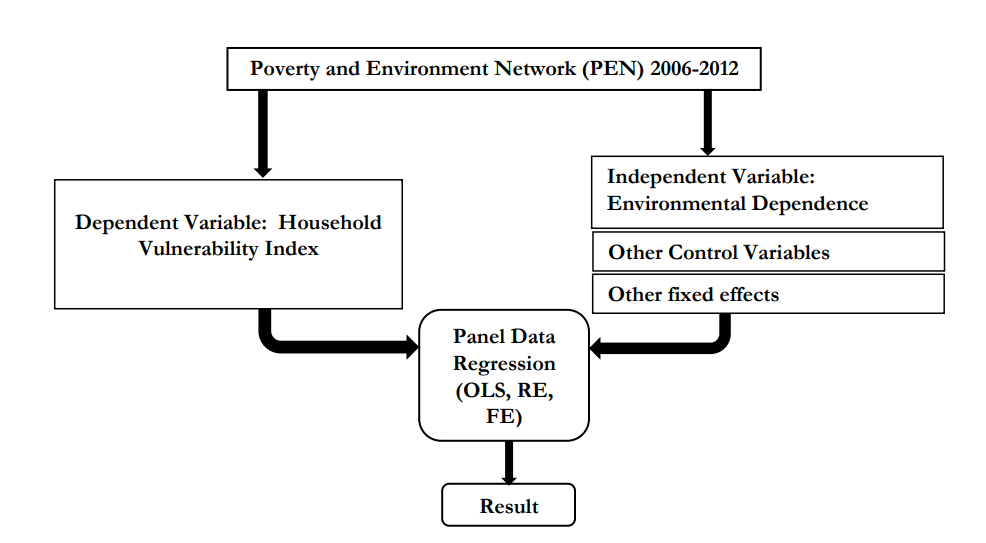
\includegraphics[scale=0.9]{Objective 2.png}
\captionsetup{labelformat=empty}
\caption{Figure 3.2: Schematic of objective two} 
\label{fig:conceptualfw2}
\setlength{\abovecaptionskip}{4pt}
\end{figure}
\\
\\
\\
\\
\\
\\
\subsection*{3.4 Sources and Nature of the Data}
\addcontentsline{toc}{subsection}{3.4 Sources and Nature of the Data}
\renewcommand{\thepage}{\arabic{page}}
\setstretch{1.5}
The sources and nature of the data are explained in this section. Further, the operationalization of the is also discussed in this section.

This study employs the A unique environmental augmented household-level livelihood panel dateset \citep{walelign2022unique} from
Nepal, Full Panel 2006-2012, produced by Tribhuvan University’s Institute of Forestry and the University of Copenhagen’s Department of Food and Resource Economics . It is a geographically representative survey spanning three main physio-graphic regions of Nepal. Data was collected in the districts of Chitwan (lowland), Kaski (mid-hills), and Mustang (mountains). Total of 507, 446 and 428 randomly sampled households were surveyed in the year 2006, 2009 and 2012 respectively. For the questionnaire see \cite{larsen2014role}. \\
The three primary physio-graphic regions of Nepal—the lowlands, mid-hills, and mountains—are covered by the study sites. The selection factors included the following: (i) Nepal's changes in elevation and vegetation; (ii) the environmental reliance of households; (iii) the attitudes of communities toward long-term research; and (iv) village accessibility and researcher safety (because of the ongoing civil conflict in Nepal at the time of site selection in 2005).\\
The data was collected through the Community Based Forest Management in the Himalaya
(ComForM) phases I - III collaborative project conducted by the Institute of Forestry (IOF) at Tribhuvan University and the Department of Food and Resource Economics (IFRO) at the University
of Copenhagen, with support from the Department of Forest Research and Survey (DFRS) at the
Ministry of Forests and Soil Conservation, Nepal. The questionnaire design was developed together with the Poverty Environment Network (PEN).\\
\begin{figure}[H]
	\centering
	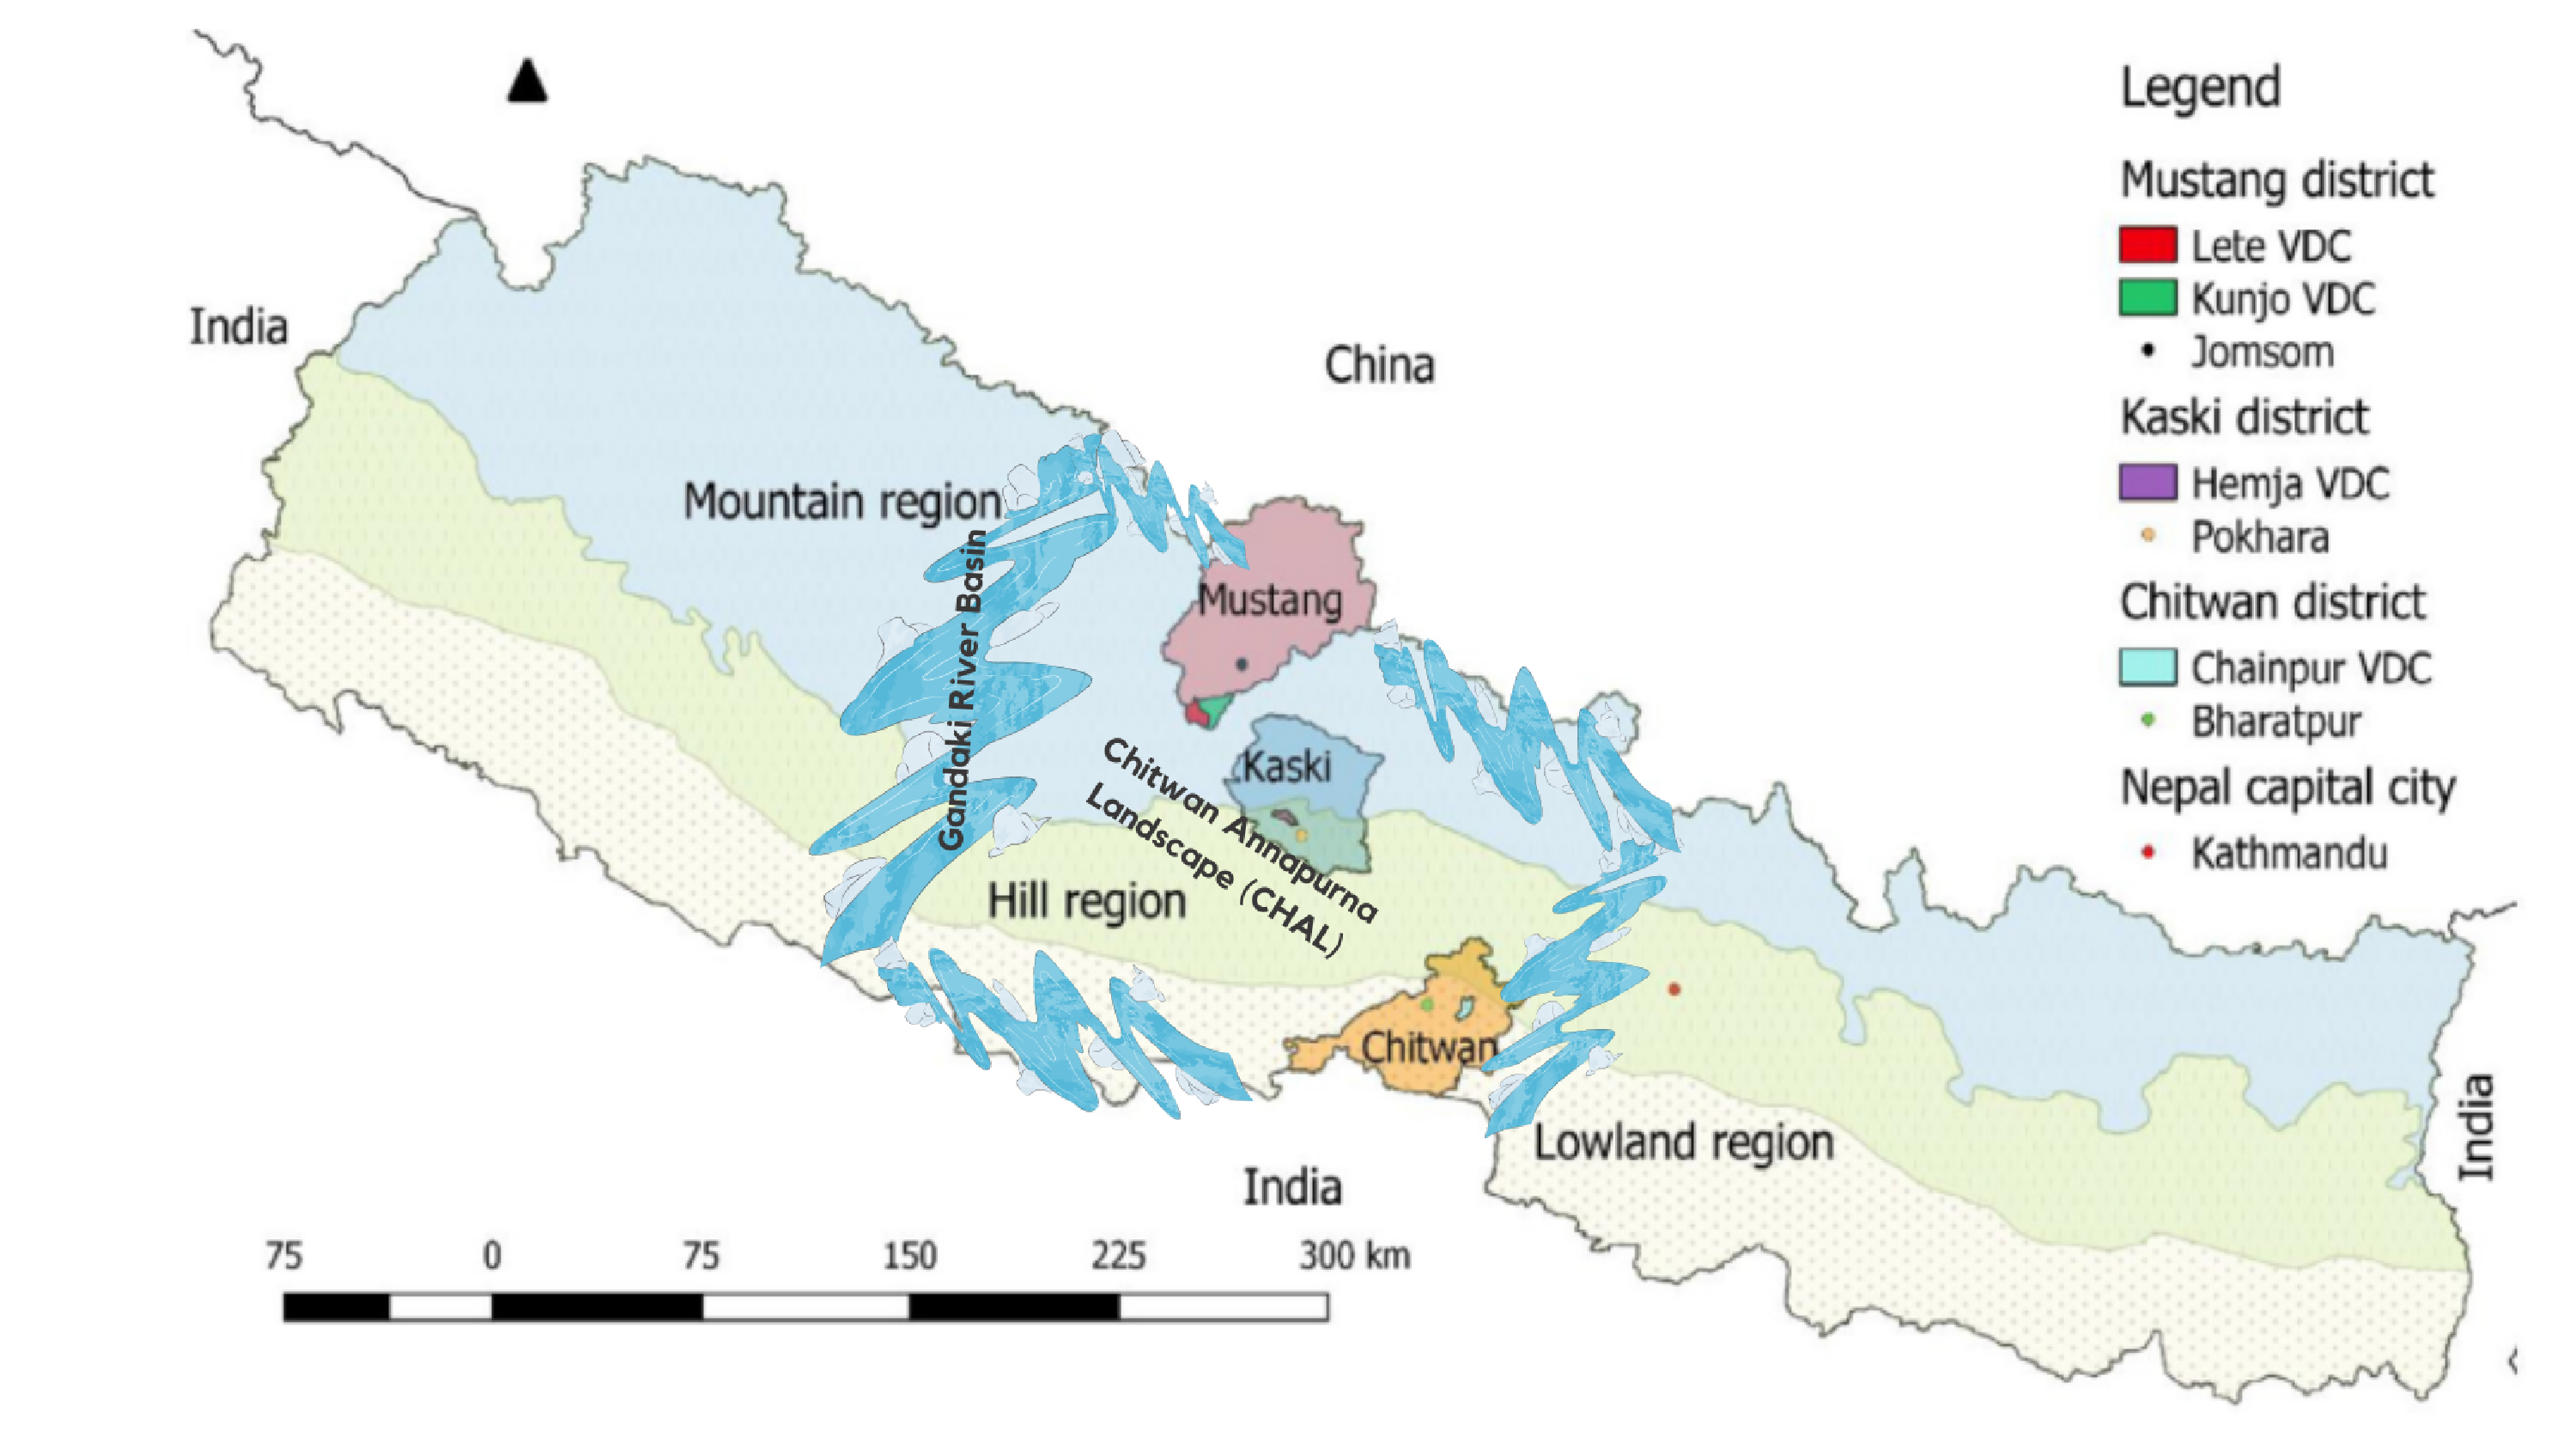
\includegraphics[scale=0.31]{Study site.png}
	\caption*{Figure 3.3: Map of the survey districts and VDCs}
	\label{fig:Surveymap}
\end{figure}

We construct the HVI as a barometer
to evaluate the level of household vulnerability at the micro
level. We constructed HVIs whose values are expressed on an interval scale
of 0-1, where the value of 0 indicates that the household is at the
minimum level of vulnerability (least vulnerable) and the value 1 indicates that the household is at the maximum vulnerability (most
vulnerable).
In order to construct the HVI, we first normalize the variables using the equations (3.5) and (3.6). The variables used are in Table 3.1. After the normalization, we grouped the variables into the group of capitals the variables belongs using equation (3.7). The we find the HVI for each household using (3.8).
\begin{singlespace}
\centering
\begin{table}[H]
	\captionsetup{labelformat=empty}
	\caption{Table 3.1: Definition of Variables used for HVI Construction}
	\vspace{0.05cm}
	\renewcommand{\arraystretch}{1.4}
	\resizebox{1.1\textwidth}{!}{%
		\begin{tabular}{p{3cm}p{12cm}} \hline \hline
			Variables & Construct \\ \hline
			hhh\_age & Household head age in years \\
			hhh\_edu & Education attainment of household head \\
			max\_hh\_edu & Highest educational attainment by a household member\\
			implements & Total value of implements such as: Car; Trucks; Motorbike; Plough etc. owned by the household in Rs.\\
			livestock & Total value of livestock (of all types) in Rs.\\
			land & Total area of land owned by the household in sq. m\\
			hh\_caste & Household belonging to the biggest caste in the village (=1) \\
			bank\_saving & Households savings kept in banks or other recognized financial institutions\\
			jewellery & Households' saving in the form of non-productive assets, such as Jewellery. \\
			n\_livelihoods & Count of livelihoods of the households \\ \hline \hline 
		\end{tabular} \\ 		
	}\\ 
	\small{\textit{Source: PEN Dataset}}
\end{table} 
\end{singlespace}
 HVI is then considered the outcome variable in the model (3.9) whereas Environmental dependence, as measured by ratio of Environmental Income to Total income of the households, is the the independent variables. Using the model, we investigate the effect of the Environmental dependence on the Household vulnerability.

\begin{center}
\begin{table}[ht]
	\renewcommand{\arraystretch}{1.2} 
	\captionsetup{labelformat=empty}
	\caption{Table 3.2: Definition of Variables affecting HVI}
	\vspace{0.05cm}
	\resizebox{1\textwidth}{!}{
		\begin{tabular}{p{3cm}p{11cm}} \hline \hline
			Variables & Construct\\ \hline
			env\_dependence & Measured by the ratio of Environmental Income to Total income of the household \\
			dependency\_ratio & Measured by the ratio of dependent and working adult members of the household \\
			debt & Debt of the household in Rs. household member \\
			n\_shocks & Count of the shocks experienced by the households \\ 
			\hline \hline 
			\end{tabular} \\
	}
	\small{\textit{Source: PEN Dataset}}
\end{table}
\end{center}
\subsection*{3.5 Techniques of Data Analysis}
\addcontentsline{toc}{subsection}{3.5 Techniques of Data Analysis}
\renewcommand{\thepage}{\arabic{page}}
\setstretch{1.5}
Household vulnerability indicators were selected after thoroughly reviewing the 
available literature.All indicators and their descriptions 
and sources are summarized in Table 3.1. The techniques of data analysis are elaborated upon in the following sections. 
\subsubsection{3.5.1. Household Vulnerability Index}
\addcontentsline{toc}{subsection}{\ \ \ \ \ 3.5.1 Household Vulnerability Index}
\renewcommand{\thepage}{\arabic{page}}
\setstretch{1.5}
To ensure the comparability of indicators that were used in the construction of the
household vulnerability index, all indicators were standardised following the
\citep{watkins2007human} procedure of standardising indicators for life expectancy index. This
ensures that all indicators were normalised to have a relative position between 0 and 1. \\
All variables with different scales are normalized with the following Min-Max standardization 
(Equations 3.5 and 3.6). Min-Max normalization helps to resize/rescale all variables analogously 
(i.e., into one scale). Here, all values are scaled between 0 and 1. Equation (3.5) applies to 
variables positively associated with vulnerability, while 
equation (3.6) applies to variables negatively associated with vulnerability. This method has been widely used in the literature related to vulnerability assessment. \cite{fang2016rural, antwi2013characterising, karunarathne2020developing, huynh2018multi, dumenu2020social} are some of the literature that have employed mini-max/maxi-min normalization technique to construct the vulnerability index.

When the variable has upward functional relationship with vulnerability, normalization was done using (3.5) and when the variable has downward functional relationship with vulnerability, normalization was done using equation (3.6):
\begin{align}
	\text{X}_{\text{ij}} &= \frac{X_{\text{i}} - X_{\text{Minj}}}{X_{\text{Maxj}} - X_{\text{Minj}}} \tag{3.5} \\[1cm] 	
	\text{X}_{\text{ij}} &= \frac{X_{\text{Maxj}} - X_{\text{i}}}{X_{\text{Maxj}} - X_{\text{Minj}}} \tag{3.6}
\end{align} 
where X is the observed value of the variable related to household i in district j, and Xmax and Xmin are 
maximum and minimum values of each variable, respectively. After normalizing all variables, 
we used equation (3.7) to calculate the final normalized index for each key component.
\begin{align}
	\text{HVI}_{\text{Cij}} &= \frac{1}{n}\sum_{i=1}^{n}\text{X}_{\text{ij}} \tag{3.7}
\end{align}
where $\text{HVI}_{\text{Cij}}$ is one of the five key components for HH. The main elements include human capital (C1), physical capital (C2), social capital (C3), livelihood (C4) and financial capital (C5). 	$\text{index}_{\text{Hvi}}$
depicts the variables of the key component indexed by C for i household in j district (while n represents the number of variables for each component). We used equation (3.8) to 
calculate the overall Hvi for the HH.
\begin{align}
	\text{HVI}_{\text{ij}} &= \sum_{i=1}^{n}\text{HVI}_{\text{Cij}} \tag{3.8}
\end{align}
where HVI is the Multi-facet Composite Household Vulnerability Index for HH x. 
C represents the numbers of key components,  indicates the weighting schemes used for the 
composite index, and n ensures the number of key components. Table 3 illustrates the weighting 
schemes used for the composite index calculated. 
\subsubsection{3.5.2. Household Vulnerability and Environmental Dependence}
\addcontentsline{toc}{subsection}{\ \ \ \ \ 3.5.2 Household Vulnerability and Environmental Dependence}
\renewcommand{\thepage}{\arabic{page}}
To examine the effect of Environmental dependence on Household vulnerability, this study employs panel estimation techniques, including pooled-OLS, fixed effects (FE), and random effects (RE) models. While simple pooled-OLS doesn't account for the time-specific or hosuehold-specific effects, the fixed effects and random effects models are designed to address such endogenity issues. Pooled-OLS is essentially a statistical regression analysis method that visually represents the relationship between data points and determines the best-fit line for a dataset. However, the fixed effects model is theoretically more suitable for cases involving unobservable individual  or household effects that may be correlated with the variables included in the model. Conversely, if individual effects are strictly uncorrelated with explanatory variables, the random effects model is a preferable choice \citep{hsiao2022analysis}.   Effect of Environmental dependence on household vulnerability is modeled using
following regression,
\vspace{-\baselineskip}
\begin{center}
	\begin{align}
\mathit{HVI}_{i,t} &= \beta_{0} + \delta \mathit{\mathbf{ED}_{i,t}} + \mathbf{X}_{i,t} \beta + \mathbf{Z}_i \lambda + \mathbf{T}_t \delta_t + \boldsymbol{\epsilon}\tag{3.9}
\end{align}
\end{center}
where, \textit{HVIi,t} is Household Vulnerability of $i^{th}$ household in \textit{t} year, \textit{EDi,t} is Environmental dependence, \textit{T} is year control variable, \textit{Xi,t} is the variables controlled for, which includes Dependency ratio, log of debt, count of shock experienced and \textit{Zi,t} represents control for time invariant
fixed effect such as district and VDCs and $\beta_{0}, \delta, \beta, \lambda, \delta_t$ are the parameter of the model.

\subsubsection{3.5.3. Diagnostic Tests}
\addcontentsline{toc}{subsection}{\ \ \ \ \ 3.5.3. Diagnostic Tests}
\renewcommand{\thepage}{\arabic{page}}
For each techniques of the Panel data analysis, we'll run few diagnostic tests to check for the effects to be included in the model such as Individual and Time effects. Also, we run the efficiency test for choosing between the models.

\subsubsection{3.5.3.1 Individual Effects Test}
\renewcommand{\thepage}{\arabic{page}}
We run the Pooled Ordinary Least Squares (OLS) regression model without considering individual effects. After obtaining the results from Pooled OLS regression, we conduct F-test to determine if there are significant individual effects (fixed effects) present in the model. We'll refer to the F-statistic and associated P-value to determine the presence of significant individual effects.  A low p-value suggests the presence of significant individual effects.

\subsubsection{3.5.3.2 Time Fixed Effects Test}
\renewcommand{\thepage}{\arabic{page}}
We also test for if there are time effects in the model. For this, we run the Pooled Ordinary Least Squares (OLS) regression model without considering individual effects. After obtaining the results from Pooled OLS regression, we conduct the Lagrange Multiplier Test - \cite{honda1988size}. It will allow us to determine if there are significant time effects (fixed effects) present in the model. We'll refer to the t-statistic and associated P-value to determine the presence of significant individual effects.  A low p-value suggests the presence of significant time effects.

\subsubsection{3.5.3.3 Breusch-Pagan Lagrange Multiplier (BPLM) Test}
\renewcommand{\thepage}{\arabic{page}}
This test is commonly referred to as Pool-ability test conducted for confirming if the cross-sectional unit in the panel has the same intercept or a different intercept. \cite{breusch1980lagrange} assesses the pool-ability of the data after incorporating the time and individual fixed effects. We'll analyze the test-statistic and associated p-value. A low p-value suggests that the data is not poolable, indicating the inadequacy of Pooled OLS regression. We'll go for Random effects (RE) regression if the p-value is low.

\subsubsection{3.5.3.4 Hausman Specification Test}
If the BP-LM test suggests that the data is not pool-able and suggests to go for Random Effects (RE) model, we'll run the RE regression. We'll also run the Fixed effects (FE) model to compare the result. After running both Random Effects (RE) and Fixed Effects (FE) models, conduct the Hausman Specification test \cite{hausman1978specification} to determine the efficient model. The test is to check whether the coefficients estimated by the two models are significantly different. We'll analyze the test statistic, typically a chi-square value, and assesses the associated p-value.  
 
\clearpage
\begin{center}
\section*{\large{CHAPTER IV \\ \vspace{-0.3cm} RESULTS AND DISCUSSION}}
\end{center}
\addcontentsline{toc}{section}{\textbf{CHAPTER IV:  RESULTS AND DISCUSSION }}
\renewcommand{\thepage}{\arabic{page}}
\setstretch{1.5}
This chapter shows the results obtained by using the methodology described in the
previous section. It also provides evidence and explanation of affecting factors of
Household Vulnerability index and how the components contribute to the household vulnerability across the years. \\


\subsection*{4.1 Descriptive Analysis}
\addcontentsline{toc}{subsection}{4.1   Descriptive Analysis}
\renewcommand{\thepage}{\arabic{page}}
The study uses household characteristics and other information from
the survey, which are more suitable for calculating the household vulnerability of the surveyed households. Table 4.1 presents various variables used for constructing the households vulnerability index district-wise. Appendix Table 1 presents the VDC-level variables.   

In the year 2006, the Household Vulnerability Index (HVI) ranged from 0.61 to 0.65 across the survey districts. By 2012, minimal changes were observed, with certain VDCs in the study districts experiencing an improvement. For instance, Chainpur VDC in Chitwan improved its vulnerability position from 0.62 in 2006 to 0.61 in 2009 but remained stagnant at 0.61 in 2012. Similarly, Kunjo VDC in Mustang district reduced its vulnerability from 0.65 in 2006 to 0.64 in 2009, but remained stagnant at 0.64 in 2012. Lete VDC in Mustang district exhibited no change in vulnerability from 2006 to 2009 but saw a decrease from 0.63 in 2006 to 0.62 in 2012. Conversely, Hemja VDC in Kaski district maintained the same vulnerability position over the six-year span. The observed phenomenon of households improving little to not improving its positions aligns with the findings of \cite{acharya2008dimension} that households in rural areas face significant vulnerability. 
\begin{landscape}
\begin{table}
	\vspace{-35pt}
	\captionsetup{labelformat=empty}
	\caption{Table 4.1: Variables used to construct the Vulnerability Index}
	\renewcommand{\arraystretch}{1.15}
\resizebox{1.7\textwidth}{!}{%
	\begin{tabular}{lccccccccc} \hline
		\textbf{Year}                    & \multicolumn{3}{c}{\textbf{2006}}                                                                                                                                                                    & \multicolumn{3}{c}{\textbf{2009}}                                                                                                                                                                    & \multicolumn{3}{c}{\textbf{2012}}                                                                                                                                                                    \\ \hline
		\textbf{District}                & \textbf{Chitwan}                                                & \textbf{Kaski}                                                  & \textbf{Mustang}                                                 & \textbf{Chitwan}                                                & \textbf{Kaski}                                                  & \textbf{Mustang}                                                 & \textbf{Chitwan}                                                & \textbf{Kaski}                                                  & \textbf{Mustang}                                                 \\ \hline
		\textbf{Human Capital}           &                                                                 &                                                                 &                                                                  &                                                                 &                                                                 &                                                                  &                                                                 &                                                                 &                                                                  \\ 
		hhh\_age                         & \begin{tabular}[c]{@{}c@{}}50.36 \\ (14.15)\end{tabular}        & \begin{tabular}[c]{@{}c@{}}50.14 \\ (14.57)\end{tabular}        & \begin{tabular}[c]{@{}c@{}}52.89  \\ (13.52)\end{tabular}        & \begin{tabular}[c]{@{}c@{}}52.13  \\ (13.75)\end{tabular}       & \begin{tabular}[c]{@{}c@{}}52.00  \\ (13.39)\end{tabular}       & \begin{tabular}[c]{@{}c@{}}54.12  \\ (13.78)\end{tabular}        & \begin{tabular}[c]{@{}c@{}}52.24  \\ (17.20)\end{tabular}       & \begin{tabular}[c]{@{}c@{}}53.52  \\ (13.71)\end{tabular}       & \begin{tabular}[c]{@{}c@{}}55.24  \\ (14.17)\end{tabular}        \\
		hhh\_edu                         & \begin{tabular}[c]{@{}c@{}}3.08  \\ (4.06)\end{tabular}         & \begin{tabular}[c]{@{}c@{}}6.29  \\ (4.97)\end{tabular}         & \begin{tabular}[c]{@{}c@{}}3.05  \\ (3.98)\end{tabular}          & \begin{tabular}[c]{@{}c@{}}2.93  \\ (4.06)\end{tabular}         & \begin{tabular}[c]{@{}c@{}}6.07  \\ (5.23)\end{tabular}         & \begin{tabular}[c]{@{}c@{}}2.94  \\ (3.78)\end{tabular}          & \begin{tabular}[c]{@{}c@{}}2.91  \\ (4.33)\end{tabular}         & \begin{tabular}[c]{@{}c@{}}6.91  \\ (5.07)\end{tabular}         & \begin{tabular}[c]{@{}c@{}}2.90  \\ (4.08)\end{tabular}          \\
		max\_hh\_edu                     & \begin{tabular}[c]{@{}c@{}}8.44  \\ (3.91)\end{tabular}         & \begin{tabular}[c]{@{}c@{}}10.76  \\ (2.90)\end{tabular}        & \begin{tabular}[c]{@{}c@{}}7.64  \\ (3.32)\end{tabular}          & \begin{tabular}[c]{@{}c@{}}9.70  \\ (3.63)\end{tabular}         & \begin{tabular}[c]{@{}c@{}}11.18  \\ (3.94)\end{tabular}        & \begin{tabular}[c]{@{}c@{}}8.04  \\ (3.93)\end{tabular}          & \begin{tabular}[c]{@{}c@{}}9.89  \\ (4.44)\end{tabular}         & \begin{tabular}[c]{@{}c@{}}11.91 \\  (4.03)\end{tabular}        & \begin{tabular}[c]{@{}c@{}}8.22  \\ (3.87)\end{tabular}          \\
		\textbf{Physical Capital}        &                                                                 &                                                                 &                                                                  &                                                                 &                                                                 &                                                                  &                                                                 &                                                                 &                                                                  \\
		implements                       & \begin{tabular}[c]{@{}c@{}}4660.32  \\ (11275.51)\end{tabular}  & \begin{tabular}[c]{@{}c@{}}14057.03  \\ (16860.40)\end{tabular} & \begin{tabular}[c]{@{}c@{}}10360.32  \\ (19629.35)\end{tabular}  & \begin{tabular}[c]{@{}c@{}}10153.80  \\ (23970.96)\end{tabular} & \begin{tabular}[c]{@{}c@{}}30700.04  \\ (46128.42)\end{tabular} & \begin{tabular}[c]{@{}c@{}}15135.16  \\ (25508.99)\end{tabular}  & \begin{tabular}[c]{@{}c@{}}22165.29  \\ (38089.26)\end{tabular} & \begin{tabular}[c]{@{}c@{}}48959.03  \\ (70582.61)\end{tabular} & \begin{tabular}[c]{@{}c@{}}21466.58  \\ (27566.06)\end{tabular}  \\
		livestock                        & \begin{tabular}[c]{@{}c@{}}18532.68  \\ (15428.31)\end{tabular} & \begin{tabular}[c]{@{}c@{}}26573.08  \\ (20411.58)\end{tabular} & \begin{tabular}[c]{@{}c@{}}80387.77  \\ (224589.10)\end{tabular} & \begin{tabular}[c]{@{}c@{}}43936.83  \\ (39679.86)\end{tabular} & \begin{tabular}[c]{@{}c@{}}35690.11  \\ (35760.04)\end{tabular} & \begin{tabular}[c]{@{}c@{}}56165.26  \\ (178639.73)\end{tabular} & \begin{tabular}[c]{@{}c@{}}38993.71  \\ (34330.39)\end{tabular} & \begin{tabular}[c]{@{}c@{}}34635.85  \\ (39306.64)\end{tabular} & \begin{tabular}[c]{@{}c@{}}34114.52  \\ (39335.73)\end{tabular}  \\
		land                             & \begin{tabular}[c]{@{}c@{}}2027.47  \\ (6367.27)\end{tabular}   & \begin{tabular}[c]{@{}c@{}}1187.00  \\ (1013.02)\end{tabular}   & \begin{tabular}[c]{@{}c@{}}2940.39  \\ (2789.36)\end{tabular}    & \begin{tabular}[c]{@{}c@{}}915.91  \\ (765.38)\end{tabular}     & \begin{tabular}[c]{@{}c@{}}1491.41  \\ (2060.26)\end{tabular}   & \begin{tabular}[c]{@{}c@{}}2235.09  \\ (3738.40)\end{tabular}    & \begin{tabular}[c]{@{}c@{}}1041.46  \\ (1136.88)\end{tabular}   & \begin{tabular}[c]{@{}c@{}}1374.96  \\ (2253.95)\end{tabular}   & \begin{tabular}[c]{@{}c@{}}1921.22  \\ (1892.77)\end{tabular}    \\
		\textbf{Social Capital}          &                                                                 &                                                                 &                                                                  &                                                                 &                                                                 &                                                                  &                                                                 &                                                                 &                                                                  \\
		hh\_caste                        & \begin{tabular}[c]{@{}c@{}}0.58  \\ (0.50)\end{tabular}         & \begin{tabular}[c]{@{}c@{}}0.89  \\ (0.32)\end{tabular}         & \begin{tabular}[c]{@{}c@{}}0.49  \\ (0.50)\end{tabular}          & \begin{tabular}[c]{@{}c@{}}0.66  \\ (0.48)\end{tabular}         & \begin{tabular}[c]{@{}c@{}}0.98  \\ (0.14)\end{tabular}         & \begin{tabular}[c]{@{}c@{}}0.58  \\ (0.50)\end{tabular}          & \begin{tabular}[c]{@{}c@{}}0.50  \\ (0.50)\end{tabular}         & \begin{tabular}[c]{@{}c@{}}0.86  \\ (0.50)\end{tabular}         & \begin{tabular}[c]{@{}c@{}}0.59 \\ (0.42)\end{tabular}           \\
		\textbf{Financial Capital}       &                                                                 &                                                                 &                                                                  &                                                                 &                                                                 &                                                                  &                                                                 &                                                                 &                                                                  \\
		bank\_saving                     & \begin{tabular}[c]{@{}c@{}}879.58  \\ (2661.50)\end{tabular}    & \begin{tabular}[c]{@{}c@{}}9663.83  \\ (26812.59)\end{tabular}  & \begin{tabular}[c]{@{}c@{}}31897.65  \\ (79933.66 )\end{tabular} & \begin{tabular}[c]{@{}c@{}}1911.63  \\ (6126.69)\end{tabular}   & \begin{tabular}[c]{@{}c@{}}11937.72  \\ (31025.90)\end{tabular} & \begin{tabular}[c]{@{}c@{}}24536.06  \\ (59338.85)\end{tabular}  & \begin{tabular}[c]{@{}c@{}}11953.55  \\ (31763.88)\end{tabular} & \begin{tabular}[c]{@{}c@{}}25410.64  \\ (66932.36)\end{tabular} & \begin{tabular}[c]{@{}c@{}}48051.24  \\ (104495.00)\end{tabular} \\
		jewellery                        & \begin{tabular}[c]{@{}c@{}}0.00  \\ (0.00)\end{tabular}         & \begin{tabular}[c]{@{}c@{}}0.00  \\ (0.00)\end{tabular}         & \begin{tabular}[c]{@{}c@{}}31662.91  \\ (67846.57)\end{tabular}  & \begin{tabular}[c]{@{}c@{}}4396.88  \\ (6965.54)\end{tabular}   & \begin{tabular}[c]{@{}c@{}}20485.87  \\ (16594.27)\end{tabular} & \begin{tabular}[c]{@{}c@{}}38598.35  \\ (79440.96)\end{tabular}  & \begin{tabular}[c]{@{}c@{}}21477.20  \\ (23620.48)\end{tabular} & \begin{tabular}[c]{@{}c@{}}51605.95  \\ (48463.66)\end{tabular} & \begin{tabular}[c]{@{}c@{}}54132.35  \\ (112328.06)\end{tabular} \\
		\textbf{Livelihood}              &                                                                 &                                                                 &                                                                  &                                                                 &                                                                 &                                                                  &                                                                 &                                                                 &                                                                  \\
		n\_livelihoods                   & \begin{tabular}[c]{@{}c@{}}4.81\\ (0.97)\end{tabular}           & \begin{tabular}[c]{@{}c@{}}4.72\\ (0.91)\end{tabular}           & \begin{tabular}[c]{@{}c@{}}4.56\\ (0.93)\end{tabular}            & \begin{tabular}[c]{@{}c@{}}4.93\\ (1.02)\end{tabular}           & \begin{tabular}[c]{@{}c@{}}4.74\\ (0.91)\end{tabular}           & \begin{tabular}[c]{@{}c@{}}5.11\\ (0.84)\end{tabular}            & \begin{tabular}[c]{@{}c@{}}4.60\\ (0.98)\end{tabular}           & \begin{tabular}[c]{@{}c@{}}4.78\\ (0.90)\end{tabular}           & \begin{tabular}[c]{@{}c@{}}4.60\\ (0.98)\end{tabular}            \\
		\textbf{Household Vulnerability} &                                                                 &                                                                 &                                                                  &                                                                 &                                                                 &                                                                  &                                                                 &                                                                 &                                                                  \\
		HVI                              & \begin{tabular}[c]{@{}c@{}}0.61  \\ (0.05)\end{tabular}         & \begin{tabular}[c]{@{}c@{}}0.62  \\ (0.04)\end{tabular}         & \begin{tabular}[c]{@{}c@{}}0.64  \\ (0.05)\end{tabular}          & \begin{tabular}[c]{@{}c@{}}0.61  \\ (0.05)\end{tabular}         & \begin{tabular}[c]{@{}c@{}}0.62  \\ (0.04)\end{tabular}         & \begin{tabular}[c]{@{}c@{}}0.63  \\ (0.05)\end{tabular}          & \begin{tabular}[c]{@{}c@{}}0.61  \\ (0.05)\end{tabular}         & \begin{tabular}[c]{@{}c@{}}0.62  \\ (0.05)\end{tabular}         & \begin{tabular}[c]{@{}c@{}}0.63  \\ (0.05)\end{tabular}         \\ \hline \hline
	\end{tabular}
}
\small{\textit{Note:SD in the parenthesis\\ [-0.9ex]
	Source: Author's Calculation}}
\end{table}
\end{landscape}

\subsection*{4.1.1 Human Capital}
Household Head Age, Education and Maximum educational attainment by the household member were taken as the Human Capital of the households. Household head age as a measure of experience and knowledge has been taken as a contributing factor in Human Capital of the households. The average age of the household head was 52 years in 2006, 53 in year 2009 and 54 in year 2012. This progression in the household head age positively affects human capital. 

On household head education, Hemja VDC of Kaski district has made a jump of 6 to 7 mean years of schooling from 2006 to 2012. Similarly, Lete VDC of Mustang district has made a negligible progress of 3.25 to 3.3 mean years of schooling. Chainpur VDC of Chitwan district and Kunjo VDC of Mustang district has made negative progress. This mixed progression of household head educational attainment will have mixed effect on human capital. 

All VDCs have made positive improvement in part of maximum educational attainment by the household members. Hemja VDC has the highest mean years of schooling of the household members. It has made a remarkable progress from 10 mean years of schooling to 12 from 2006 to 2012. Chainpur VDC also has followed the similar trajectory. It had mean of 8 years of schooling in 2006 and it improved to 10 by the end of 2012. Lete VDC had 8.14 mean years of schooling in the year 2006 which only slightly improved to 8.7 in the year 2012. Kunjo VDC has the least mean years of educational attainment by the household member with 7.1 years in 2006 to 7.72 in 2012. The improvement in the schooling years would affect the human capital positively.

\subsection*{4.1.2 Physical Capital}
Chainpur VDC had the least implements in the year 2006 whereas Hemja had the highest level of implements in the same year. But, chainpur made remarkable progress by increasing its implements by 118\%  by the end of 2009 and exactly the same increase by the end of the year 2012. Hemja also experience the same rate of growth of implements in the year 2009 but the rate declined to 59\% in the year 2012. Kunjo and Lete, both VDC of Mustang could improve its implements position in the year 2009 by 77\% and 32\% respectively. However, both VDC had a decline in the growth of the implements in the last wave of the survey. Kunjo's increase of the implements was 69\% and Lete's was only 25\%. 

In part of Livestock holdings, Lete VDC had the highest holding in the year 2006 whereas Chainpur had the least holding of the livestock. However, Chainpur managed to increase its livestock-holding by 137\% at the end of year 2009. But Chainpur VDC's livestock holding declined by 11\% by the end of 2012. Kunjo was the second place after Lete in the livestock holding in year 2006. But, its livestock-holding declined continuously in the following years 2009 and 2012 by 25\% and 11\% respectively. Lete VDC despite holding the most livestock in the year 2006 had a severe decline in its livestock holding placing itself as the least livestock-holding VDC by the end of year 2012. It experienced the decrease of 33\% in the year 2009 and almost 60\% in the year 2012. 

Lete VDC had the highest land holding followed by Kunjo VDC in the year 2006. Kaski had the least land holdings in the same year. Chainpur then followed Kaski. In year 2009, Chainpur had a decline of 55\% whereas Kunjo and Lete had a decline of 14\% and 33\% respectively. Hemja, however, increased its land-holding by 26\% by the end of 2009. Chainpur, despite experiencing decrease in land-holding, managed to increase the land-holding by 14\% by the end of 2012. In the same period, all 3 VDCs': Hemja; Kunjo; and Lete experienced decline in the land-holding by 8\%, 13\% and 15\% respectively. 

All of these fluctuations in the physical capital holding is going to alter the household vulnerability.  

\subsection*{4.1.3 Social Capital}  
Following \cite{alha2018other, vanneman2006social}, the caste was considered as a social capital. Belonging to the largest caste improves the household's network within the community as well as across the community. Thus it helps the households to negate the effects of uncertain events. So, belonging to largest caste have a negative influence on the household vulnerability. In the year 2006 Hemja had the highest percentage of Household head i.e. 89\% belonging to largest caste. Whereas Kunjo had the least percentage of the household heads belonging to the largest caste in the village. The trend followed with increase in the percentage of the household heads belonging to the largest caste in the year 2009. Chainpur, Hemja, Kunjo and Lete had the percentage change of household heads belonging to largest caste increase by 13\%, 10\%, 19\% and 17\% respectively. 

However, the percentage change declined by 23\% and 48\% for Chainpur and Hemja respectively in the year 2012. Kunjo and Lete, however experience an increase of the percentage of household heads belonging to caste by 65\% and 8\% in the year 2012 respectively. 

\subsection*{4.1.4 Financial Capital}
Bank savings and Jewellery are considered as the financial capitals. The financial capital play a huge part in the welfare of the households. 

Lete VDC had the highest bank savings in the year 2006 and the trend continued until the final wave of the survey year 2012. It experienced decline of the saving in the year 2009 relative to 2006 by 11\% but it managed to increase its saving by 114\% by the end of 2012. Chainpur had a opposite experience than that of Lete. It had the least bank saving among all VDCs in the year 2006 and it persisted to have least of it in the final wave of the survey year 2012. However, it managed to increase its own saving by 117\% in the year 2009 and 525\% by the end of 2012. 

Kunjo had a fairly fluctuating trend with respect to bank saving. It followed Lete to have the second highest possession of bank saving in the year 2006. Though it managed to maintain the position in terms of ranking it had a decline of 41\% in the second of wave of survey year 2009. In the following wave of the survey it experienced an increase of savings by 54\%. But, it fell below the previous ranking. Hemja had a moderate growth of its saving in the year 2009 of 24\%. The rate leaped to 113\% by the end of 2012.     

The data for jewellery possession were not available for Chainpur and Hemja VDC for the year 2006. So comparing between Kunjo and Lete, Lete had the highest possession of jewellery. It continued to have the highest jewellery possession in the following wave of surveys. The rate of increase remained moderate of 13\% and 22\% in the year 2009 and 2012 respectively. Kunjo, on the other hand, have aggressively increased its jewellery possession by 45\% in the year 2009 and 80\% in the year 2012. 

Data for jewellery possession were available for Chainpur and Hemja for 2009 and 2012. Chainpur had the least possession in the year 2009. But, it managed to increased its possession by 388\% in the year 2012 which is the highest rate of increase among all VDCs. Nonetheless, it persisted in the VDC having the least possession of jewellery in the final wave of survey year 2012.  

 
 \subsection*{4.1.5 Livelihood Options} 
 This includes the diversity of livelihood options that the households in the particular area in the particular period of time. The livelihood is considered a capital because having diversified income can raise household income, reduce risk, and improve their livelihoods \citep{scoones2013livelihoods}. All of the VDCs have a relatively similar livelihood counts. In the year 2006, the number of livelihood strategies that the households adopted ranged from 4.32 to 4.81. Kunjo had the least number of livelihood strategies while Chainpur had a relatively more number of strategies. The average number of livelihood strategies have increased in the year 2009. But, the rate of increase is fairly mild for Chainpur with only 2\% increase and Hemja with only 0.4\%.  As for Kunjo, it had an increase of 11\% in their livelihood counts. Lete had an increase of 12\% in the year 2009. In the year 2012, all VDCs except for Hemja experienced downward sloping livelihood counts. Hemja observed a growth of 0.84\% in livelihood strategies, while Chainpur, Kunjo, and Lete exhibited reduced growth rates of 7\%, 11\%, and 8\%, respectively. 

  
\subsection*{4.2 Environmental Dependence and Household Vulnerability}
\addcontentsline{toc}{subsection}{4.2 Environmental Dependence and Household Vulnerability}
\renewcommand{\thepage}{\arabic{page}}  
Table 4.2 presents the factors that are likely to affect Household vulnerability with central emphasis on Environmental dependence. The table consists of four critical variables which are assumed to affect the household vulnerability. The definition of the variables are in Table 3.2. The variables are: Environmental dependence; Dependency ratio; and Shock.


\begin{table}[H]
	\captionsetup{labelformat=empty}
	\caption{Table 4.2: Household Vulnerability and Environmental Dependence}
	\renewcommand{\arraystretch}{0.9}
	\resizebox{0.9\linewidth}{!}{
		\begin{center}
	\begin{tabular}{llcccc} \hline
		\multicolumn{2}{l}{\textbf{Year}}     & \multicolumn{4}{c}{\textbf{2006}}                                                                                                                                                                                                                                 \\ \hline
		\multicolumn{2}{l}{\textbf{District}} & \textbf{Chitwan}                                               & \textbf{Kaski}                                                 & \textbf{Mustang}                                               & \textbf{Mustang}                                               \\ \hline
		\multicolumn{2}{l}{\textbf{VDC}}      & \textbf{Chainpur}                                              & \textbf{Hemja}                                                 & \textbf{Kunjo}                                                 & \textbf{Lete}                                                  \\ \hline
		\multicolumn{2}{l}{env\_dependence}   & \begin{tabular}[c]{@{}c@{}}0.13\\      (0.19)\end{tabular}     & \begin{tabular}[c]{@{}c@{}}0.16\\      (0.20)\end{tabular}     & \begin{tabular}[c]{@{}c@{}}0.40\\      (0.23)\end{tabular}     & \begin{tabular}[c]{@{}c@{}}0.29\\      (0.23)\end{tabular}     \\
		\multicolumn{2}{l}{dependency\_ratio} & \begin{tabular}[c]{@{}c@{}}0.66\\      (0.62)\end{tabular}     & \begin{tabular}[c]{@{}c@{}}0.73\\      (0.76)\end{tabular}     & \begin{tabular}[c]{@{}c@{}}0.88\\      (0.85)\end{tabular}     & \begin{tabular}[c]{@{}c@{}}0.69\\      (0.63)\end{tabular}     \\
		\multicolumn{2}{l}{debt}              & \begin{tabular}[c]{@{}c@{}}12234.42\\ (19246.56)\end{tabular}  & \begin{tabular}[c]{@{}c@{}}25896.24\\ (47371.72)\end{tabular}  & \begin{tabular}[c]{@{}c@{}}17792.57\\ (19055.29)\end{tabular}  & \begin{tabular}[c]{@{}c@{}}31217.37\\  (69576.58)\end{tabular} \\
		\multicolumn{2}{l}{shock}             & \begin{tabular}[c]{@{}c@{}}1.75\\      (1.66)\end{tabular}     & \begin{tabular}[c]{@{}c@{}}0.55\\      (1.07)\end{tabular}     & \begin{tabular}[c]{@{}c@{}}2.48\\      (1.24)\end{tabular}     & \begin{tabular}[c]{@{}c@{}}1.97\\      (1.2)\end{tabular}      \\ \Xhline{0.9pt}
		\multicolumn{2}{l}{\textbf{Year}}     & \multicolumn{4}{c}{\textbf{2009}}                                                                                                                                                                                                                                 \\ \hline
		\multicolumn{2}{l}{env\_dependence}   & \begin{tabular}[c]{@{}c@{}}0.14\\      (0.23)\end{tabular}     & \begin{tabular}[c]{@{}c@{}}0.13\\      (0.15)\end{tabular}     & \begin{tabular}[c]{@{}c@{}}0.19\\      (0.30)\end{tabular}     & \begin{tabular}[c]{@{}c@{}}0.21\\      (0.59)\end{tabular}     \\
		\multicolumn{2}{l}{dependency\_ratio} & \begin{tabular}[c]{@{}c@{}}0.58\\      (0.56)\end{tabular}     & \begin{tabular}[c]{@{}c@{}}0.63\\      (0.63)\end{tabular}     & \begin{tabular}[c]{@{}c@{}}0.77\\      (0.64)\end{tabular}     & \begin{tabular}[c]{@{}c@{}}0.68\\      (0.69)\end{tabular}     \\
		\multicolumn{2}{l}{debt}              & \begin{tabular}[c]{@{}c@{}}18249.69\\  (36642.37)\end{tabular} & \begin{tabular}[c]{@{}c@{}}46654.49\\  (72705.08)\end{tabular} & \begin{tabular}[c]{@{}c@{}}14887.21\\  (16156.9)\end{tabular}  & \begin{tabular}[c]{@{}c@{}}20616.94\\ (41324.71)\end{tabular}  \\
		\multicolumn{2}{l}{shock}             & \begin{tabular}[c]{@{}c@{}}0.24\\      (0.65)\end{tabular}     & \begin{tabular}[c]{@{}c@{}}0.59\\      (0.96)\end{tabular}     & \begin{tabular}[c]{@{}c@{}}0.65\\      (1.00)\end{tabular}     & \begin{tabular}[c]{@{}c@{}}1.16\\      (1.14)\end{tabular}     \\ \Xhline{0.9pt}
		\multicolumn{2}{l}{\textbf{Year}}     & \multicolumn{4}{c}{\textbf{2012}}                                                                                                                                                                                                                                 \\ \hline
		\multicolumn{2}{l}{env\_dependence}   & \begin{tabular}[c]{@{}c@{}}0.15\\      (0.20)\end{tabular}     & \begin{tabular}[c]{@{}c@{}}0.14\\      (0.25)\end{tabular}     & \begin{tabular}[c]{@{}c@{}}0.78\\      (3.16)\end{tabular}     & \begin{tabular}[c]{@{}c@{}}0.27\\      (0.25)\end{tabular}     \\
		\multicolumn{2}{l}{dependency\_ratio} & \begin{tabular}[c]{@{}c@{}}0.51\\      (0.60)\end{tabular}     & \begin{tabular}[c]{@{}c@{}}0.53\\      (0.57)\end{tabular}     & \begin{tabular}[c]{@{}c@{}}0.77\\      (0.82)\end{tabular}     & \begin{tabular}[c]{@{}c@{}}0.49\\      (0.56)\end{tabular}     \\
		\multicolumn{2}{l}{debt}              & \begin{tabular}[c]{@{}c@{}}37221.48\\ (87094.30)\end{tabular}  & \begin{tabular}[c]{@{}c@{}}64572.68\\ (133587.15)\end{tabular} & \begin{tabular}[c]{@{}c@{}}24507.84\\  (33242.18)\end{tabular} & \begin{tabular}[c]{@{}c@{}}19864.55\\ (27238.68)\end{tabular}  \\
		\multicolumn{2}{l}{shock}             & \begin{tabular}[c]{@{}c@{}}0.77\\      (1.01)\end{tabular}     & \begin{tabular}[c]{@{}c@{}}0.31\\      (0.66)\end{tabular}     & \begin{tabular}[c]{@{}c@{}}0.35\\      (0.72)\end{tabular}     & \begin{tabular}[c]{@{}c@{}}0.24\\      (0.59)\end{tabular}  \\ \hline \hline  
	\end{tabular} 
\end{center}
}
{\textit{\ \ \ \ \ \ \ \ \ \ \ \  Note: Standard deviation in the parenthesis \\ [-1ex] Source: Author's Calculation}}
\end{table}

\subsection*{4.2.1 Environmental Dependence}
From the table, Kunjo VDC had a highest dependence on environment for its livelihood in the year 2006 and 2012. Lete VDC followed Kunjo in the dependence on environment. Both of the VDC continued to persist on a higher level of environmental dependence across all waves of survey years. Kunjo and Lete VDC's dependency decreased in the year 2009 by 27\% and 52\% respectively. However, the dependency increased by a notably significant 78\% for Kunjo and only 28\% for Lete in the year 2012. 

Chainpur had the least dependency on environment in the year 2006. Hemja had only slightly higher dependence on environment in the same year. Chainpur had a mild increase of 8\% in dependency in the year 2009 whereas Hemja had a decline of 18\% in the dependency. However, in the year 2012, both of the VDCs had similar mild rate of increase in dependence of 7\% and 8\% respectively.

Chainpur and Hemja VDC's environmental dependence in relatively lower in comparison to Kunjo and Lete. Kunjo, in particular had a relatively higher environmental dependence. This evident difference of environmental dependence in the physio-graphic regions implies that communities in the upper belt are more environmentally dependent. This tendency can be credited to the availability the livelihood options to these communities \citep{rayamajhi2012empirical, larsen2014role}. The environmental dependence is expected to contribute to household vulnerability positively.           
\subsection*{4.2.2 Dependency Ratio}
In the year 2006, the dependency ratio for Kunjo VDC is the highest and lowest for Chainpur. The dependency ratio has declined continuously in all of the VDCs across all 3 waves of the survey period. Only Kunjo VDC had a consistent level of dependency ratio in the year 2009 and 2012.The dependency ratio is expected to affect the household vulnerability positively. 

\subsection*{4.2.3 Debt}
Lete VDC is the highest indebted VDC in the year 2006 with average of Rs. 31,217.40 debt. However, the debt declined to Rs. 20,616.94 in the year 2009 and Rs. 19,864.55 in the year 2012. Chainpur VDC had the lowest debt in the year 2006. But, the debt increased to Rs. 18,249.69 in the year 2009 and Rs. 37,221.48 in the year 2012. Hemja also had its debt increase from Rs. 25,896.24 in year 2006 to Rs. 46,654.49 in year 2009 and to Rs. 64,572.68 in the year 2012. Kunjo, however had a mixed trend of indebtedness. It had a declining trend from the debt of Rs. 17,792.57 in the year 2006 to Rs.14,887.21 in the year 2009. But, the debt increased to Rs. 24,507.84 by the end of 2012.

Although being indebted is not a ideal position to be in rural setting, particularly when the household doesn't have regular flow of income to service the debt. However, households in rural setting resort to acquiring debts to stay away from the situation that could worsen the vulnerability. In the short run, the debt could reduce the vulnerability when exposed to shocks. In this regard, debt is expected to reduce the vulnerability of the household.   

\subsection*{4.2.4 Shock}
Shocks like Crop failure, Serious Illness, Death of an adult member of family, Land loss, Livestock loss, Other assets loss, Wage employment loss, Costly Social Events are included in the count of the shocks. This includes all forms of severity from less severe to more severe shock. When a shock occurs in the community or household, they lose their assets that might be in the form of saving or other form of assets which increases their vulnerability \citep{dercon2006vulnerability}. 

Counting the number of shocks experienced by the household across the survey years, Kunjo VDC of Mustang district had experienced relatively higher number of shocks with an average of 2.48 as compared to its counterparts in the year 2006. Lete VDC of the same district followed it with the average of 1.97 number of shocks in the same year. Both of the VDCs had lower number of shocks in the following wave of survey in the year 2009. Kunjo had a significantly lower drop of 74\% in the number of shock experienced. It only had an average of 0.65 in the year 2009. Lete also had an decrease of 41\% in the number of shocks experienced in the year 2009. Both of the VDCs had a significant drop in the number of shocks experienced in the final wave of survey year 2012. Lete was the VDC with the least number of shocks experienced by the end of the year 2012.

Chainpur  had a fairly fluctuating average of shocks experienced. Its count of shocks was 1.75, 0.24 and 0.77 in the respective waves of 2006, 2009 and 2012. It experienced a lower number of shocks in 2009 relative to 2006. However, the shocks increased in 2012 relative to 2009. But, the count is lower relative to 2006.
Hemja had a different trend. The number of shocks increased to 0.59 from 0.55 from 2006 to 2009. Nonetheless, the number decreased to 2012.
      
The expected effect of shock on household vulnerability is positive. As the number of shock increases, the households become more vulnerable and vice-versa.

\subsection*{4.3 District and Village level Household Vulnerability}
\addcontentsline{toc}{subsection}{4.3 District and Village level Household Vulnerability}
\renewcommand{\thepage}{\arabic{page}} 
 
Table 4.3 presents data on the average household vulnerability Index for different districts across three distinct years: 2006, 2009, and 2012. The districts include Chitwan, Kaski, and Mustang.

In 2006, the mean HVI in Chitwan, Kaski, and Mustang were 0.62, 0.62, and 0.64, respectively. Similarly, in 2009, the mean HVI for the mentioned districts were 0.61, 0.62, and 0.63. The trend continues in 2012, with mean of 0.61, 0.62, and 0.63 for Chitwan, Kaski, and Mustang, respectively.

This allows for an analysis of the variability in the household vulnerability Index within each district across the specified years, providing insights into the distribution of household vulnerability levels over time.
\begin{table}[H]
	\captionsetup{labelformat=empty}
	\caption{Table 4.3: District level mean and SD HVI for all waves}
	\label{tab:districtlevelhvi}
	\resizebox{\textwidth}{!}{%
		\begin{tabular}{cccccccccc} \hline
			\multirow{2}{*}{\textbf{\begin{tabular}[c]{@{}c@{}}Year/\\ District\end{tabular}}} & \multicolumn{3}{c}{\textbf{2006}}                                                                                                                                     & \multicolumn{3}{c}{\textbf{2009}}                                                                                                                                     & \multicolumn{3}{c}{\textbf{2012}}                                                                                                                                     \\ \hline
			& \textbf{Chitwan}                                      & \textbf{Kaski}                                        & \textbf{Mustang}                                      & \textbf{Chitwan}                                      & \textbf{Kaski}                                        & \textbf{Mustang}                                      & \textbf{Chitwan}                                      & \textbf{Kaski}                                        & \textbf{Mustang}                                      \\ \hline
			\textbf{HVI}                                                                       & \begin{tabular}[c]{@{}c@{}}0.62\\ (0.05)\end{tabular} & \begin{tabular}[c]{@{}c@{}}0.62\\ (0.04)\end{tabular} & \begin{tabular}[c]{@{}c@{}}0.64\\ (0.05)\end{tabular} & \begin{tabular}[c]{@{}c@{}}0.61\\ (0.05)\end{tabular} & \begin{tabular}[c]{@{}c@{}}0.62\\ (0.04)\end{tabular} & \begin{tabular}[c]{@{}c@{}}0.63\\ (0.05)\end{tabular} & \begin{tabular}[c]{@{}c@{}}0.61\\ (0.05)\end{tabular} & \begin{tabular}[c]{@{}c@{}}0.62\\ (0.05)\end{tabular} & \begin{tabular}[c]{@{}c@{}}0.63\\ (0.05)\end{tabular} \\ \hline \hline
	\end{tabular}
}
{\textit{\ \ \ \ Note: Standard deviation in the parenthesis \\ [-1ex] \ \ \ \ \ \ \ \ Source: Author's Calculation}}
\end{table}
Figure 4.1 is a radar chart, also known as a spider chart or web chart, is a graphical method of displaying multivariate data in the form of two-dimensional chart. In our analysis, the radar chart represents the District level mean HVI values across the 3-waves of survey from 2006-2012 with 3 years gap in each interval. 

Each axis in the radar chart represents wave of survey (2006, 2009 and 2012). The data points on each axis correspond to the mean HVI values for the respective districts (Chitwan, Kaski and Mustang). The lines connect the data points for each district, forming a polygon or shape in the chart. The area enclosed by the lines represents the range or variability of the mean HVI values for each district.

Chitwan district had a mildly variable vulnerability level across the waves of survey. It had mean HVI of 0.62 in the first wave of the survey which declined to 0.61 in the second and remained constant in the third wave of the survey. The polygon enclosed by the lines from the HVI data points indicates that the variability of HVI is mildly variable across the points. 

Kaski district also had a stable vulnerability with a mean HVI of 0.62. This exhibits a stability of vulnerability over the years for Kaski district. 

Mustang district had mean HVI of 0.64 in the year 2006, indicating relatively higher household vulnerability in other survey districts. Moving to 2009 the HVI slightly decreased to 0.63. In 2012, the HVI remained stable completing the polygon with HVI of 0.63. This demonstrates the slight variability in the HVI in the first transition from 2006 to 2009. However, the polygon stabilized from 2009 to 2012 with a consistent HVI. 

The examination of Chitwan's, Kaski's, and Mustang's polygons reveals distinct characteristics in variability. A stable polygon for Chitwan implies consistent mean HVI, while subtle shifts in Kaski's polygon suggest a potential decrease in variability. Mustang's polygon, displaying variability followed by stabilization, hints at fluctuations.  
\begin{figure}[H]
	\vspace{-180pt} % Adjust the value as needed to reduce space above the figure
	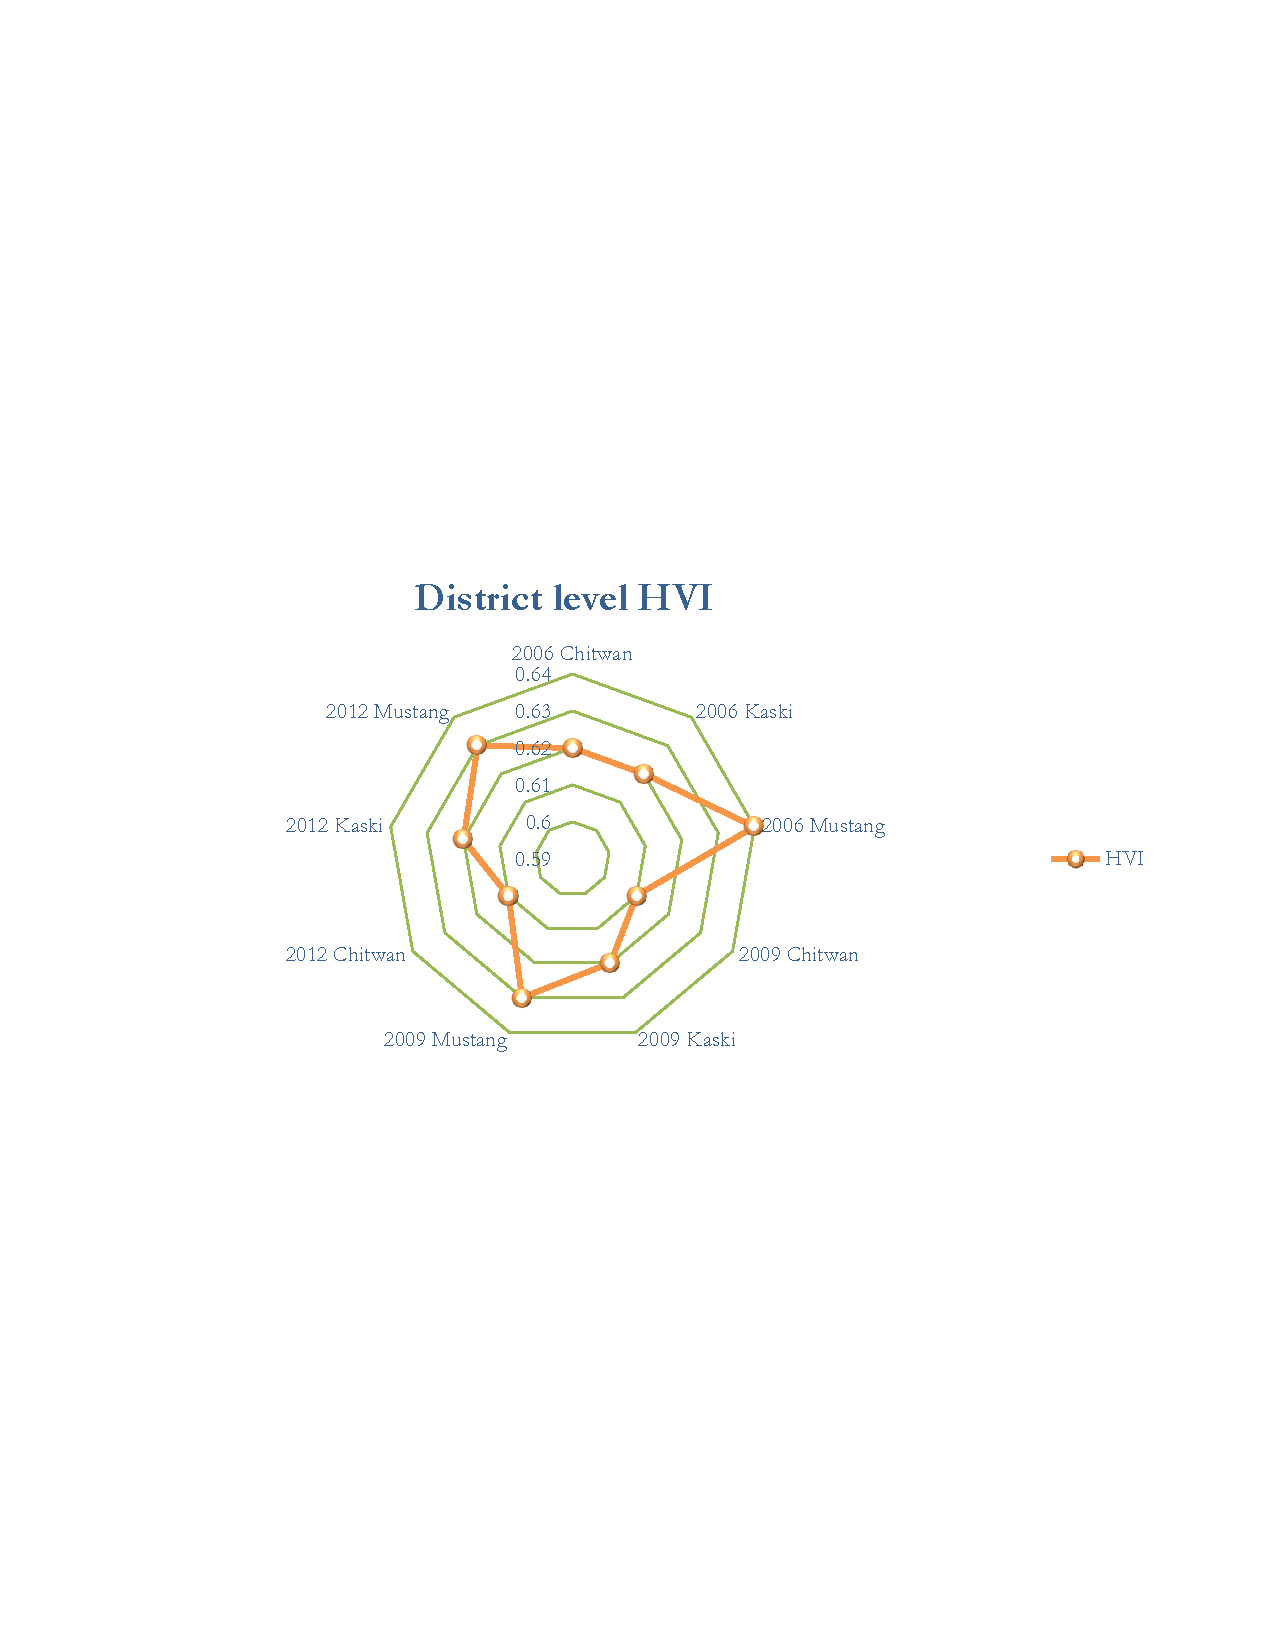
\includegraphics[scale=0.8]{HVI_Summary_District_Panel1.pdf}
	\captionsetup{labelformat=empty, aboveskip=1pt}% Adjust belowskip to reduce caption space
	\vspace{-160pt}
	\caption{Figure 4.1: District level HVI for all waves} 
	\label{fig:distictlevelhvi}
	\setlength{\abovecaptionskip}{6pt}
	\label{fig:conceptualfw}
\end{figure}

Table 4.4 represents household vulnerability Index (HVI) values for different Village Development Committees (VDC) across three districts (Chitwan, Kaski and MUstang) for three distinct years: 2006, 2009, and 2012. The VDCs within each district are Chainpur, Hemja, Kunjo, and Lete. The HVI values are provided for each combination of VDC and year.

\begin{table}[H]
	\captionsetup{labelformat=empty} % remove the automatic caption and sets it empty
	\caption{Table 4.4: Village level mean and SD HVI for all waves}
	\label{vdclevelhvi}
	\resizebox{\textwidth}{!}{%
		\begin{tabular}{cccclccclcccl} \hline
			\multirow{2}{*}{\textbf{\begin{tabular}[c]{@{}c@{}}Year/\\ District\end{tabular}}} & \multicolumn{4}{c}{\textbf{2006}}                                                                                                                                                                                             & \multicolumn{4}{c}{\textbf{2009}}                                                                                                                                                                                             & \multicolumn{4}{c}{\textbf{2012}}                                                                                                                                                                                             \\ \hline
			& \textbf{Chainpur}                                     & \textbf{Hemja}                                        & \textbf{Kunjo}                                        & \textbf{Lete}                                         & \textbf{Chainpur}                                     & \textbf{Hemja}                                        & \textbf{Kunjo}                                        & \textbf{Lete}                                         & \textbf{Chainpur}                                     & \textbf{Hemja}                                        & \textbf{Kunjo}                                        & \textbf{Lete}                                         \\ \hline
			\textbf{HVI}                                                                       & \begin{tabular}[c]{@{}c@{}}0.62\\ (0.05)\end{tabular} & \begin{tabular}[c]{@{}c@{}}0.62\\ (0.04)\end{tabular} & \begin{tabular}[c]{@{}c@{}}0.65\\ (0.04)\end{tabular} & \begin{tabular}[c]{@{}l@{}}0.63\\ (0.05)\end{tabular} & \begin{tabular}[c]{@{}c@{}}0.61\\ (0.05)\end{tabular} & \begin{tabular}[c]{@{}c@{}}0.62\\ (0.04)\end{tabular} & \begin{tabular}[c]{@{}c@{}}0.64\\ (0.04)\end{tabular} & \begin{tabular}[c]{@{}l@{}}0.63\\ (0.05)\end{tabular} & \begin{tabular}[c]{@{}c@{}}0.61\\ (0.05)\end{tabular} & \begin{tabular}[c]{@{}c@{}}0.62\\ (0.05)\end{tabular} & \begin{tabular}[c]{@{}c@{}}0.64\\ (0.05)\end{tabular} & \begin{tabular}[c]{@{}l@{}}0.62\\ (0.05)\end{tabular} \\ \hline \hline
		\end{tabular}
	}
	{\textit{\ \ \ \ Note: Standard deviation in the parenthesis \\ [-1ex] \ \ \ \ \ \ \ \ Source: Author's Calculation}}
\end{table}

In 2006, the mean HVI in Chainpur, Hemja, Kunjo and Lete were 0.61, 0.62, 0.65 and 0.64, respectively. Similarly, in 2009, the mean HVI for the mentioned VDCs were 0.61, 0.61, 0.64 and 0.63. The trend continued in 2012, with mean HVI of 0.61, 0.62, 0.63 and 0.61 for the above-mentioned VDCs respectively.

We present the radar chart for the Village level mean HVI for all the VDCs across the survey years.

The radar chart for Chainpur shows a polygon with points relatively close to each other, suggesting a stable pattern in HVI across the years. The HVI for Chainpur was 0.62 in the first wave of the survey. The HVI then declined to 0.61 and has remained stable across the second and third waves of survey. Similarly, Hemja's radar chart exhibit a relatively stable HVI across all waves of survey. The HVI has remained at 0.62 across all the waves of survey. \vspace{-1.5cm}
\begin{center}
\begin{figure}[H]
	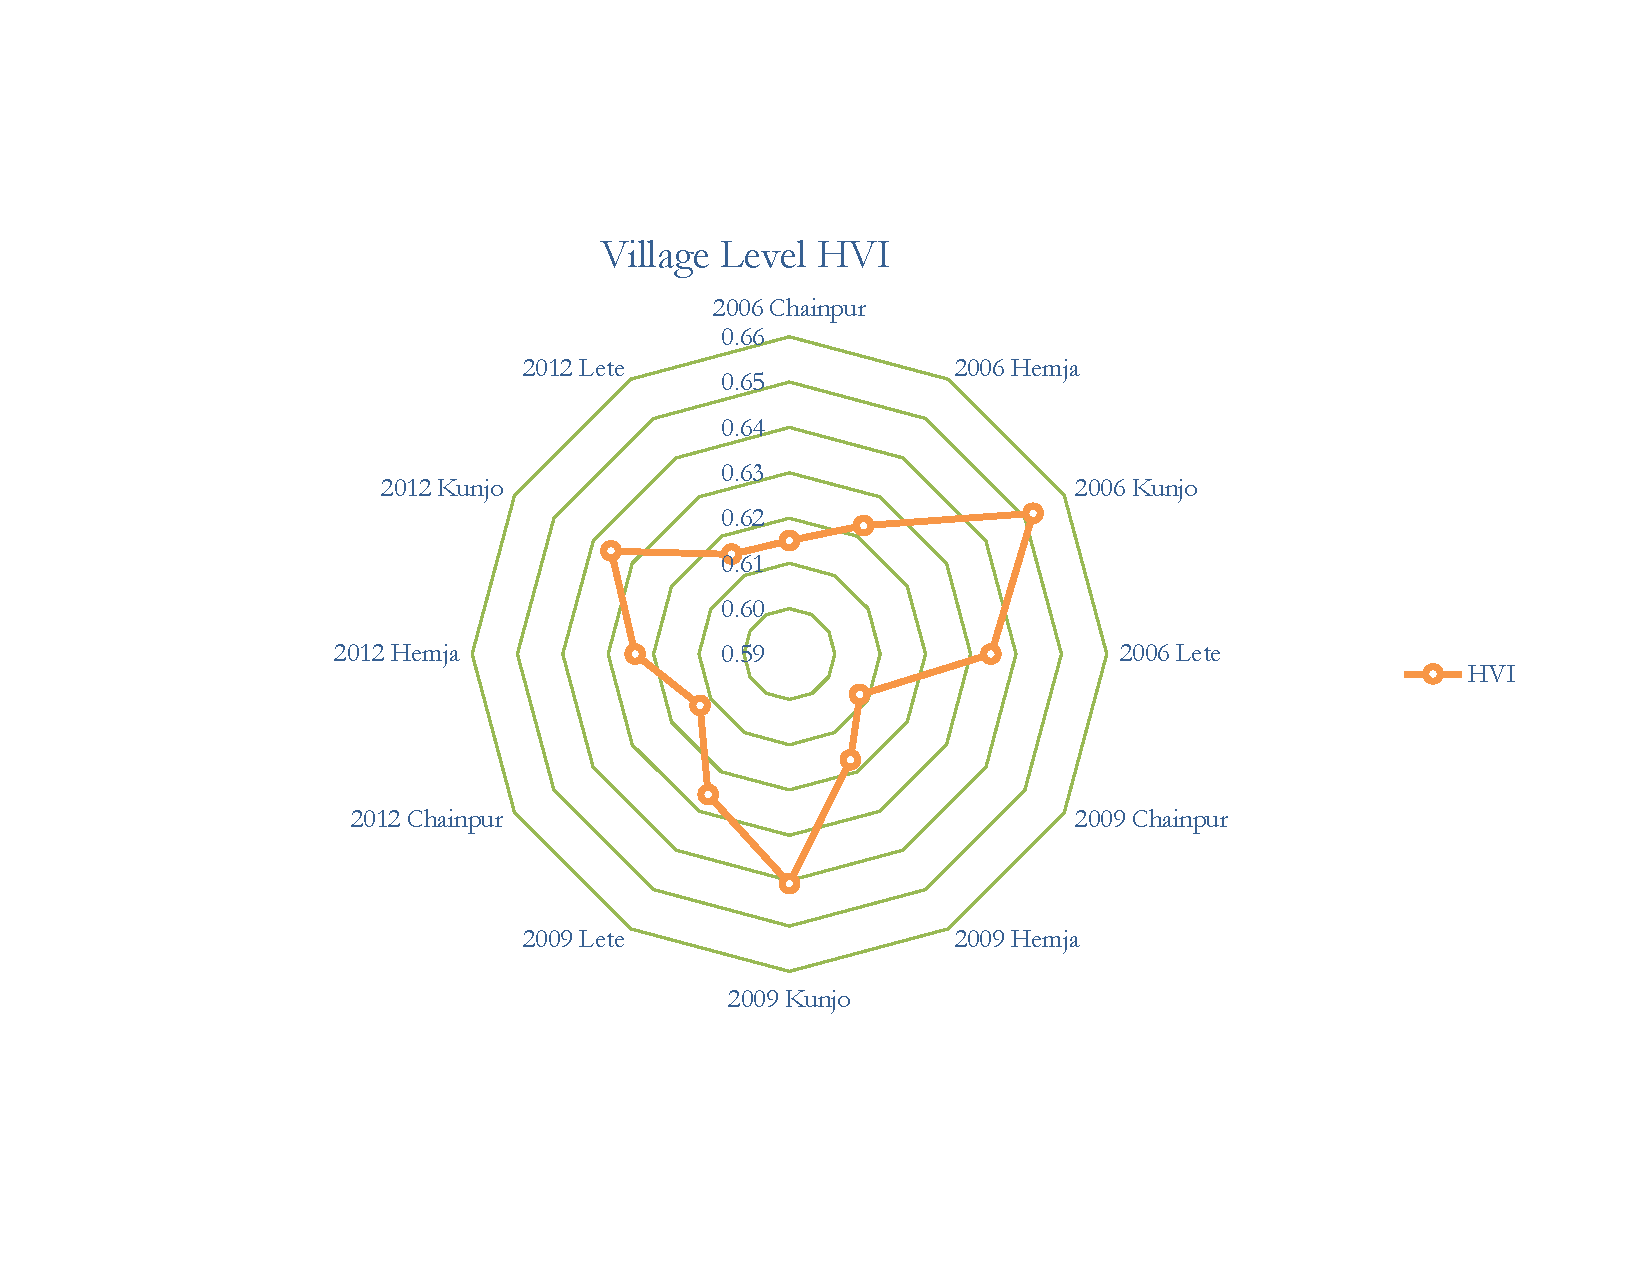
\includegraphics[scale=0.62]{HVI_Summary_VDC1.pdf}
	\vspace{-1.5cm}
		\captionsetup{labelformat=empty}
			\caption{Figure 4.2: Village level HVI for all waves} 
	\label{fig:vdclevelhvi}
	\setlength{\belowcaptionskip}{6pt}
	\label{fig:conceptualfw}
\end{figure}
\end{center}
\vspace{-0.5cm}
Kunjo was the highest vulnerable VDC among all the VDC. Lete followed it in terms of the vulnerability. Kunjo formed a mildly varying polygon. The HVI declined by 0.01 in 2009 from 2006. Then the HVI remains stable at 0.64 from year 2009 to 2012. The VDC had 0.65, 0.64 and 0.64 HVI in the year 2006, 2009 and 2012 respectively. This steady variation has formed a slightly fluctuating polygon.  Lete's HVI was 0.63 in the 2006 which remained consistent in the year 2009. However, it declined to 0.62 in the year 2012.   
\subsection*{4.4 Components of the Household Vulnerability}
\addcontentsline{toc}{subsection}{4.4 Component of the Household Vulnerability}
\renewcommand{\thepage}{\arabic{page}}
\subsection*{4.4.1 Chainpur VDC, Chitwan}
\ \ \ \ \ Table 4.5 represents Chainpur VDC data for different years (2006, 2009, 2012) and various components of vulnerability, categorized into five types of capital: Human Capital (C1), Physical Capital (C2), Social Capital (C3), Livelihoods (C4), and Financial Capital (C5). The variables used in each component is in the Table 3.1. The value for the capital has been derived from equation 3.7.

\begin{center}
\begin{table}[]
	\captionsetup{labelformat=empty}
	\caption{Table 4.5: Mean of the HVI components for Chainpur VDC, Chitwan}
	\label{tab:hvicomponentforchainpur}
		\resizebox{1\textwidth}{!}{%
	\begin{tabular}{ccccccc} \hline
		\textbf{Year} & \textbf{\begin{tabular}[c]{@{}c@{}}Human Capital\\  (C1)\end{tabular}} &  \textbf{\begin{tabular}[c]{@{}c@{}}Physical Capital \\ (C2)\end{tabular}} & \textbf{\begin{tabular}[c]{@{}c@{}}Social Capital \\ (C3)\end{tabular}} & \textbf{\begin{tabular}[c]{@{}c@{}}Livelihoods \\ (C4)\end{tabular}} & \textbf{\begin{tabular}[c]{@{}c@{}}Financial Capital \\ (C5)\end{tabular}} \\ \hline
		\textbf{2006} & 0.63                                                                      &  0.98                                                                         & 0.68                                                                       & 0.31                                                                 & 0.99                                                                          \\
		\textbf{2009} & 0.60                                                                                                                                                     & 0.98                                                                         & 0.72                                                                       & 0.30                                                                 & 0.99                                                                          \\
		\textbf{2012} & 0.60                                                                                                                                                     & 0.97                                                                         & 0.63                                                                       & 0.34                                                                 & 0.98   \\ \hline \hline                                                                     
	\end{tabular}
}
	\textit{Source: Author's Calculation}
\end{table}
\end{center}
\vspace{-25pt}
 Fig 4.3 exhibits how each component has contributed to the vulnerability level of the households in Chainpur, Chitwan. Having higher Human capital reduces vulnerability. Human Capital is exhibited to have slight decrease from 0.63 in 2006 to 0.60 in 2009 and 2012 in Chainpur. This implies that the decline in the Human capital had a negative effect on household vulnerable. Physical capital remained relatively stable around 0.98 across all rounds of survey years, suggesting a consistent level of vulnerability related to physical assets. Social Capital is demonstrated to have some variation, increasing from 0.68 in 2006 to 0.72 in 2009 and then decline to 0.63 in the year 2012. This suggests that this variation could potentially have some effect on the overall vulnerability of the household. In the livelihood component, depicts a slight dip to 0.30 in the year 2009 fro 0.31 in the year 2006. However, livelihood component have increased to 0.34 in the year 2012. Financial capital have remained stable at around 0.99 across 2006 and 2009 and only slightly decreasing to 0.98 in the year 2012. 
   
\begin{center}
\begin{figure}[H]
	\vspace{-140pt}
	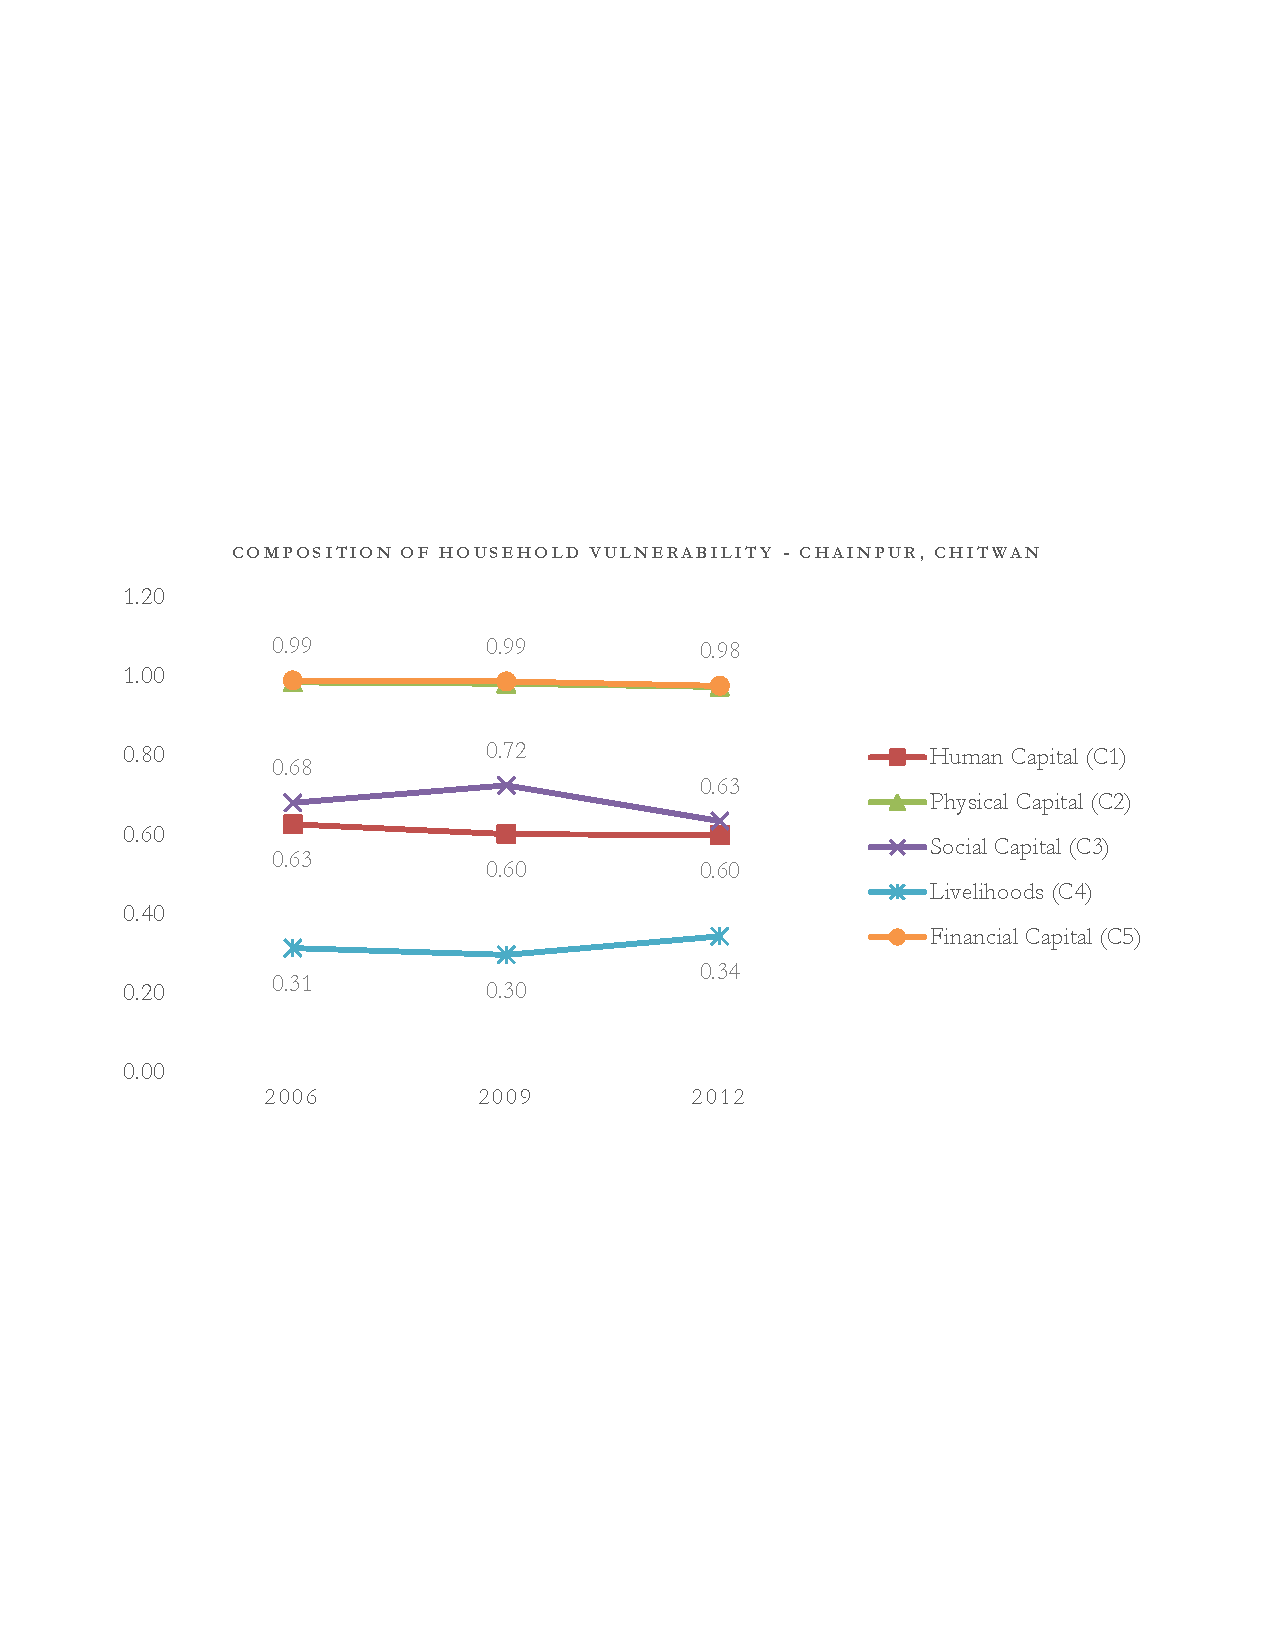
\includegraphics[scale=0.7]{HVI_Component_Chainpur1.pdf}
	\captionsetup{labelformat=empty, belowskip=0.01pt}
	\vspace{-160pt}
	\caption{Figure 4.3: Component of HVI - Chainpur VDC, Chitwan}
	\setlength{\abovecaptionskip}{6pt}
	\setlength{\belowcaptionskip}{3pt}
	\label{fig:hvichainpurComponent}
\end{figure}
\end{center}
\vspace{-25pt}
\subsection*{4.4.2 Hemja VDC, Kaski}
Table 4.6 represents data for Hemja Village Development Committee (VDC) in Kaski district across the years 2006, 2009, and 2012.
\begin{table}[ht]
	\captionsetup{labelformat=empty}
		\caption{Table 4.6: Mean of the HVI components for Hemja VDC, Kaski}
		\resizebox{1\textwidth}{!}{%
	\begin{tabular}{ccccccc} \hline
		\textbf{Year} & \textbf{\begin{tabular}[c]{@{}c@{}}Human Capital\\  (C1)\end{tabular}} &  \textbf{\begin{tabular}[c]{@{}c@{}}Physical Capital \\ (C2)\end{tabular}} & \textbf{\begin{tabular}[c]{@{}c@{}}Social Capital \\ (C3)\end{tabular}} & \textbf{\begin{tabular}[c]{@{}c@{}}Livelihoods \\ (C4)\end{tabular}} & \textbf{\begin{tabular}[c]{@{}c@{}}Financial Capital \\ (C5)\end{tabular}} \\ \hline
		\textbf{2006} & 0.53                                                                      &  0.98                                                                         & 0.84                                                                       & 0.33                                                                 & 0.99                                                                          \\
		\textbf{2009} & 0.52                                                                      &  0.97                                                                         & 0.87                                                                       & 0.32                                                                 & 0.98                                                                          \\
		\textbf{2012} & 0.49                                                                                                                                                     & 0.95                                                                         & 0.62                                                                       & 0.32                                                                 & 0.96 \\      \hline  \hline                                                                \end{tabular}
	}
	\textit{Source: Author's calculation}
		\end{table}

Figure 4.4 shows the representation of different components of vulnerability. Human Capital decreases steadily from 0.53 in 2006 to 0.52 in 2009 and further to 0.49 in 2012 in Hemja VDC over the specified years. Physical capital is exhibited a gradual decrease from 0.98 in 2006 to 0.97 in 2009 to 0.95 in 2012. Social capital also have experienced an increase from 0.84 in 2006 to 0.87 in 2009 and declined to 0.62 in 2012.Livelihoods Remains relatively stable, ranging from 0.32 to 0.33 across the three years. Financial Capital also remained relatively stable with a slight decrease from 0.99 in 2006 to 0.96 in 2012. 

Hemja VDC in Kaski district exhibits a vulnerability profile characterized by a decline in human and physical capital over the years. Social capital shows variability, with a decline from 2006 to 2012. Livelihoods and financial capital remain relatively stable. 
\begin{figure}[ht]
	\vspace{-50pt}
	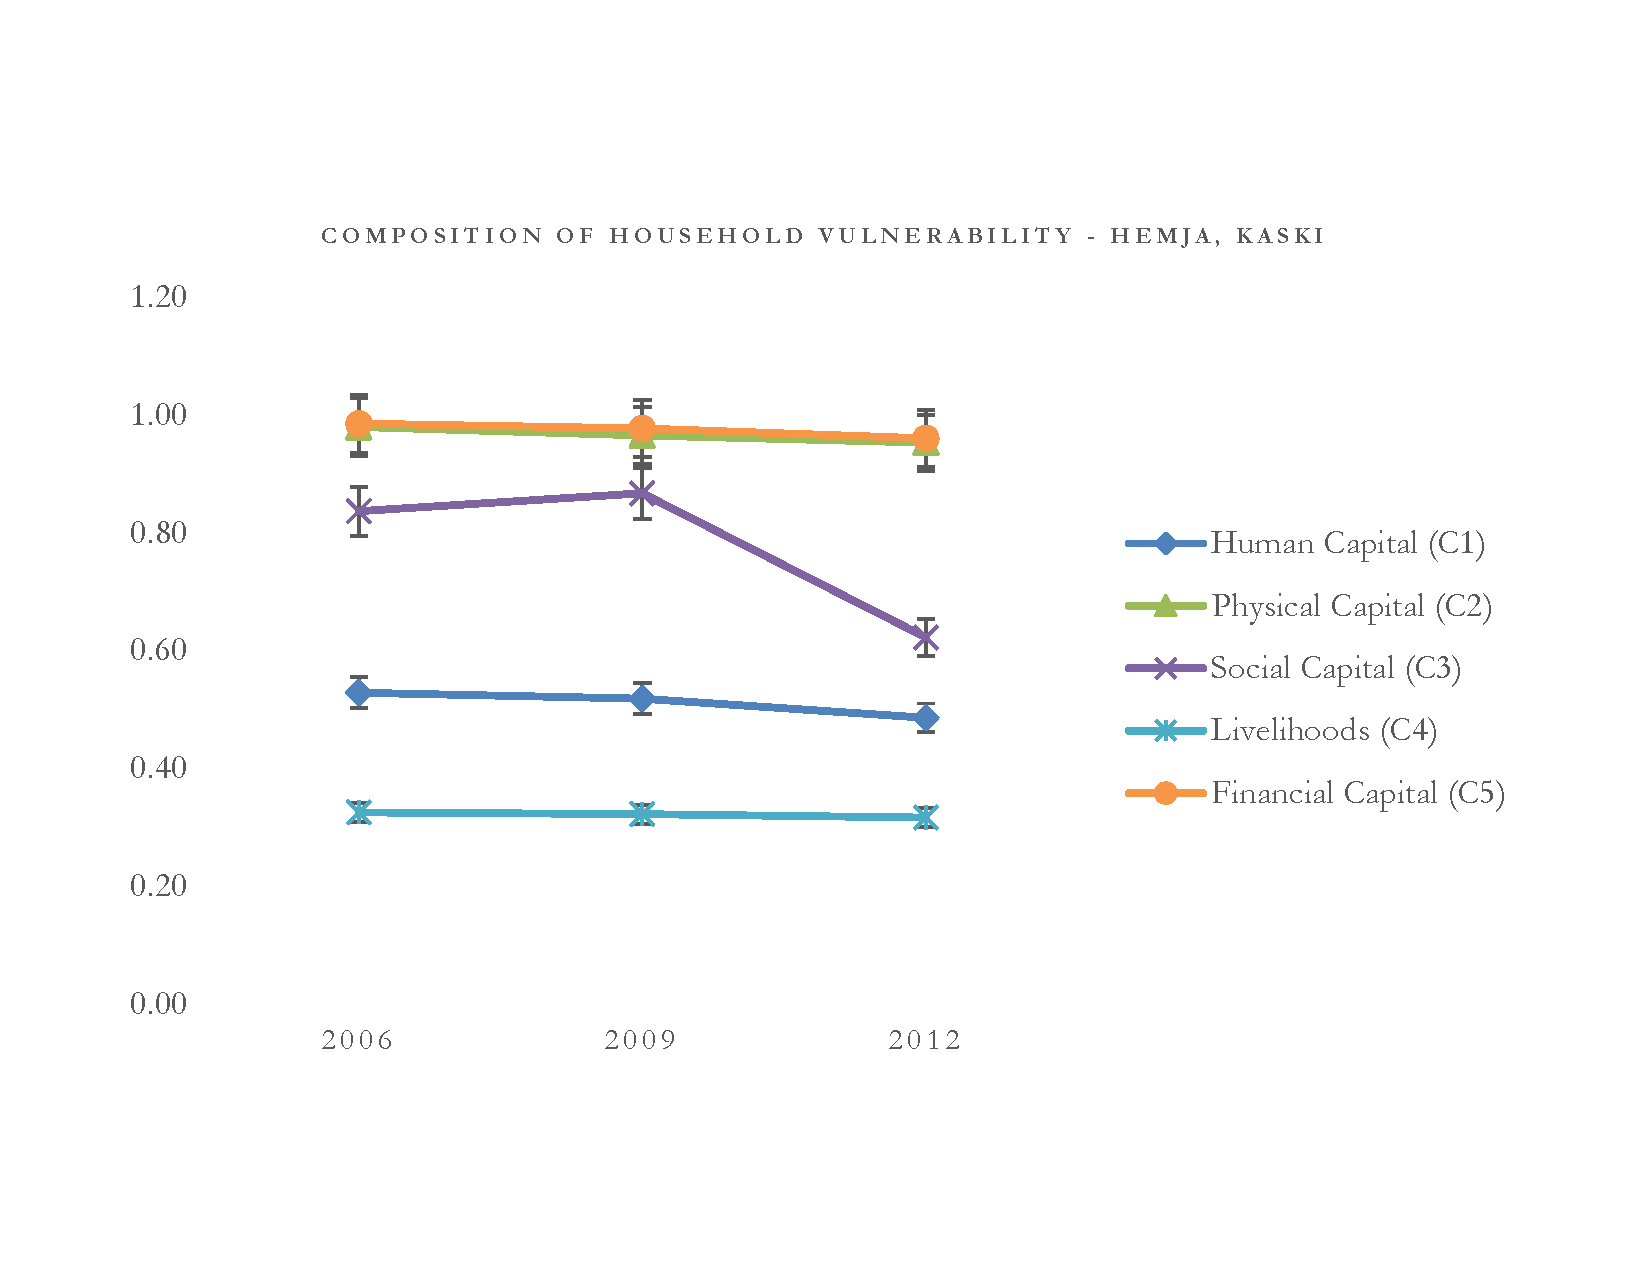
\includegraphics[scale=0.6]{HVI_Component_Hemja1.pdf}
		\captionsetup{labelformat=empty}
			\vspace{-50pt} % reduce the gap below the figure before caption
	\caption{Figure 4.4: Component of HVI - Hemja VDC, Kaski}
	\setlength{\abovecaptionskip}{4pt}
	\label{fig:hvihemjacomponent}
\end{figure}

\subsection*{4.4.3 Kunjo VDC, Mustang}
Table 4.7 represents data for Kunjo Village Development Committee (VDC) in Mustang district across the years 2006, 2009, and 2012. Each row corresponds to a specific year, and the columns represent different components of vulnerability.
\begin{table}[ht]
	\captionsetup{labelformat=empty}
		\caption{Table 4.7: Mean of the HVI components for Kunjo VDC, Mustang}
		\label{tab:hvikunjocomponents}
		\resizebox{1\textwidth}{!}{%
	\begin{tabular}{ccccccc} \hline
		\textbf{Year} & \textbf{\begin{tabular}[c]{@{}c@{}}Human Capital\\  (C1)\end{tabular}} &  \textbf{\begin{tabular}[c]{@{}c@{}}Physical Capital \\ (C2)\end{tabular}} & \textbf{\begin{tabular}[c]{@{}c@{}}Social Capital \\ (C3)\end{tabular}} & \textbf{\begin{tabular}[c]{@{}c@{}}Livelihoods \\ (C4)\end{tabular}} & \textbf{\begin{tabular}[c]{@{}c@{}}Financial Capital \\ (C5)\end{tabular}} \\ \hline
		\textbf{2006} & 0.65                                                                      &  0.97                                                                         & 0.59                                                                       & 0.31                                                                 & 0.97                                                                          \\
		\textbf{2009} & 0.63                                                                      &  0.97                                                                         & 0.63                                                                       & 0.24                                                                 & 0.97                                                                          \\
		\textbf{2012} & 0.64                                                                      &  0.97                                                                         & 0.82                                                                       & 0.32                                                                 & 0.96  \\ \hline \hline                                                                      
\end{tabular} 
}		
\textit{Source: Author's calculation}
\end{table}
Human capital component was 0.65 in 2006, decreases to 0.63 in 2009, and slightly increases to 0.64 in 2012. Physical capital remains constant at 0.97 across all three years. Social capital component 0.59 in 2006, increases to 0.63 in 2009, and further increases to 0.82 in 2012. Livelihood components exhibits variability across the years. The average value decreased to 0.24 in 2009 from 0.31 in 2006 and then increasing to 0.32 in 2012. Financial capital remained relatively stable at around 0.97 across three years. 

Overall, Human capital and financial capital exhibited slight fluctuations. Physical capital remained stable. Social capital experienced a significant increase. Livelihood show variability with a dip in 2009 and subsequent increase in 2012.     	
\begin{figure}[ht]
	\vspace{-40pt}
	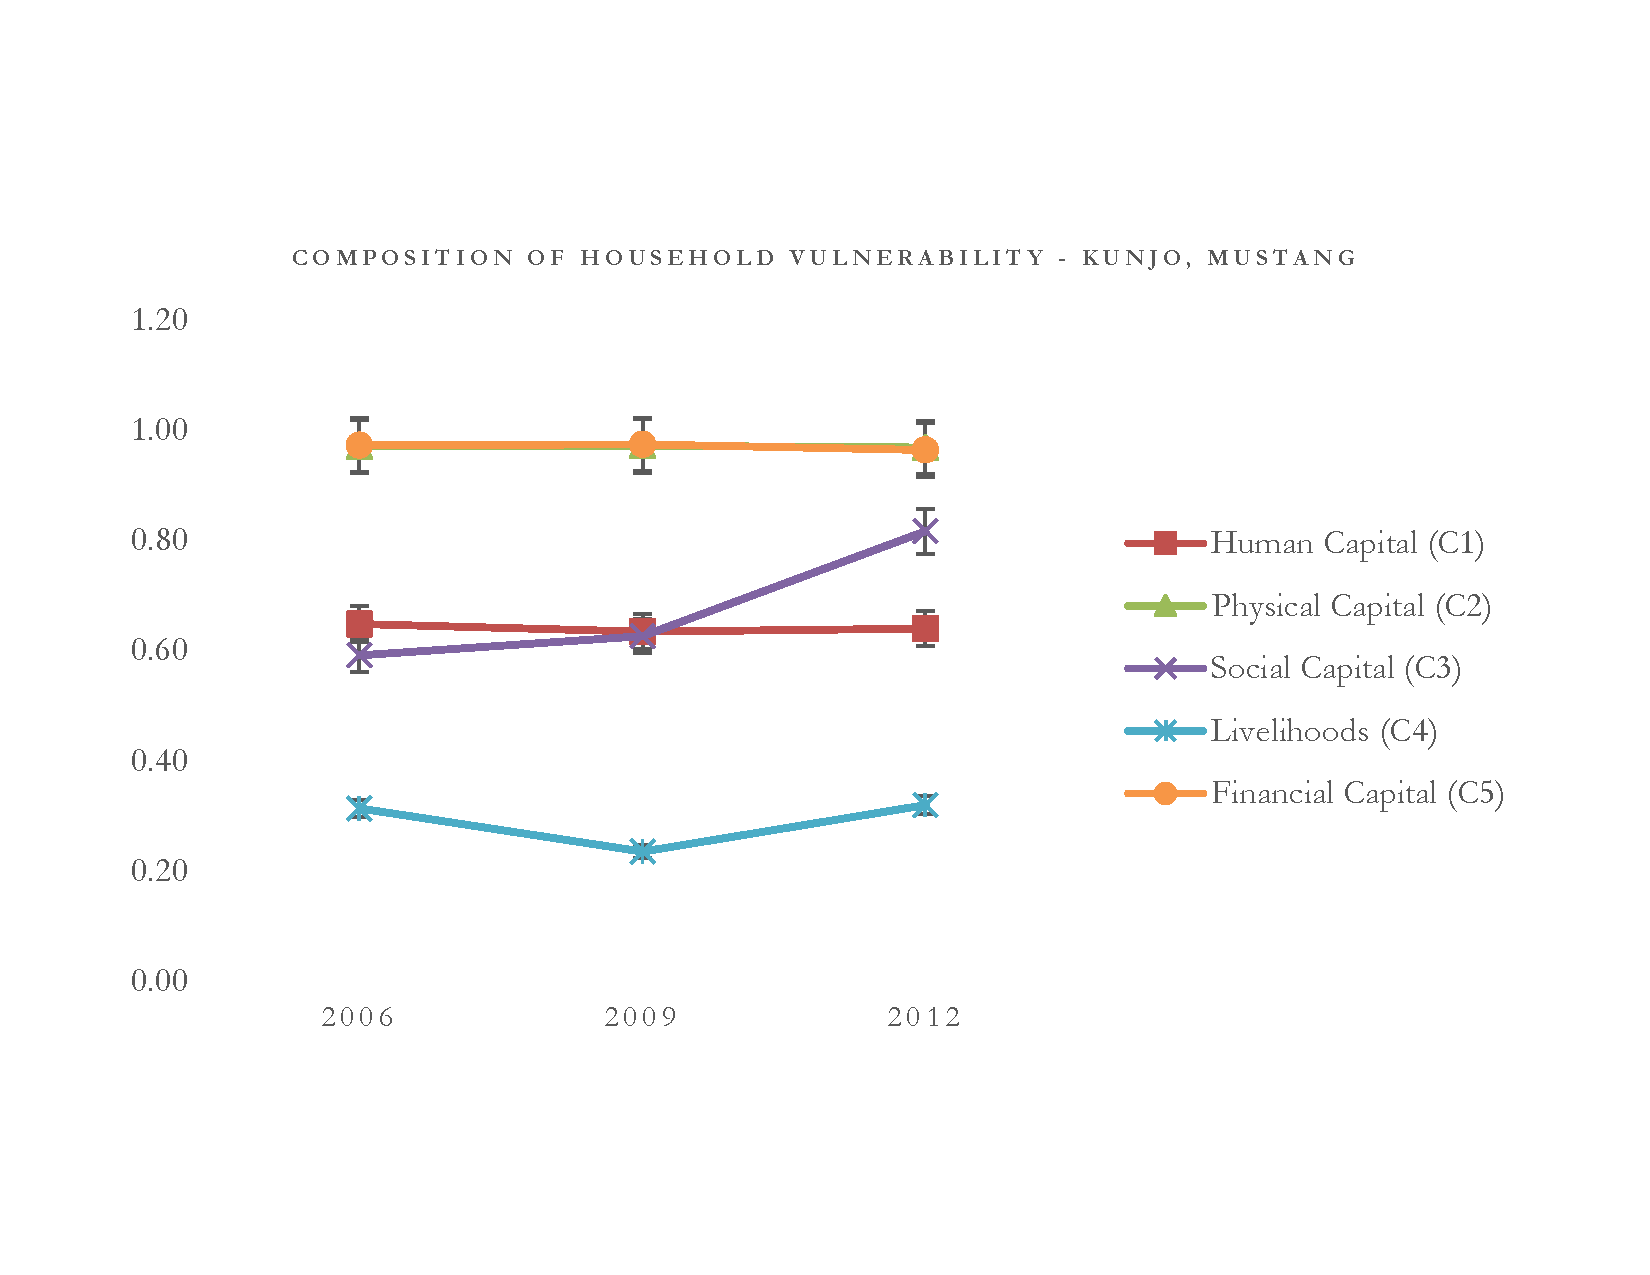
\includegraphics[scale=0.6]{HVI_Component_Kunjo1.pdf}
	\vspace{-50pt}
	\captionsetup{labelformat=empty}
	\caption{Figure 4.5: Component of HVI - Kunjo VDC, Mustang}
	\setlength{\abovecaptionskip}{4pt}
	\label{fig:hvikunjocomponents}
\end{figure}

\subsection*{4.4.4 Lete VDC, Mustang}
The table represents data for Lete Village Development Committee (VDC) in Mustang district across the years 2006, 2009, and 2012. Each row corresponds to a specific year, and the columns represent different components of vulnerability.
\begin{table}[ht]
	\captionsetup{labelformat=empty}
	\caption{Table 4.8: Mean of the HVI components for Lete VDC, Mustang}
	\label{tab:hviletecomponents}
		\resizebox{1\textwidth}{!}{%
	\begin{tabular}{ccccccc} 
		\hline
		\textbf{Year} & \textbf{\begin{tabular}[c]{@{}c@{}}Human Capital\\  (C1)\end{tabular}} &  \textbf{\begin{tabular}[c]{@{}c@{}}Physical Capital \\ (C2)\end{tabular}} & \textbf{\begin{tabular}[c]{@{}c@{}}Social Capital \\ (C3)\end{tabular}} & \textbf{\begin{tabular}[c]{@{}c@{}}Livelihoods \\ (C4)\end{tabular}} & \textbf{\begin{tabular}[c]{@{}c@{}}Financial Capital \\ (C5)\end{tabular}} \\ \hline
		\textbf{2006} & 0.61                                                                      &  0.96                                                                         & 0.66                                                                       & 0.38                                                                 & 0.96                                                                          \\	\textbf{2009} & 0.61                                                                      &  0.97                                                                         & 0.69                                                                       & 0.31                                                                 & 0.96                                                                          \\ \textbf{2012} & 0.59                                                                      &  0.97                                                                         & 0.70                                                                       & 0.36                                                                 & 0.94 \\ \hline  \hline                                                            		\end{tabular} 
	}
	\textit{Source: Author's calculation}
\end{table}
Human Capital indicates stability with a minor decline in. The human capital component was 0.61 in 2006, remains constant in the following year, and slightly decreases to 0.59 in the year 2012. Physical Capital suggests stability and a slight improvement. The physical capital increases from 0.96 in 2006 to 0.97 in the year 2009 and remains constant in 2012. Social Capital is exhibited to have consistent rise across the years. It was 0.66 in the year 2006, increases to 0.69 in the year 2009, and further increases to 0.70 in the year 2012. Livelihoods component is fluctuating across the years. Livelihood decrease from 0.38 in 2006 to 0.31 in 2009, and then increasing to 0.36 in 2012. Financial capital indicates generally stable but slightly declining level of vulnerability related to financial resources. Financial Capital component was 0.96 in 2006, remained constant in 2009, and decreased slightly to 0.94 in 2012. 

We could observe stability in physical capital and social capital with minor fluctuations. human capital and financial capital exhibited a minor decline. Livelihood showed variability with a dip in one wave and increase in another wave. 
 
\begin{figure}[H]
	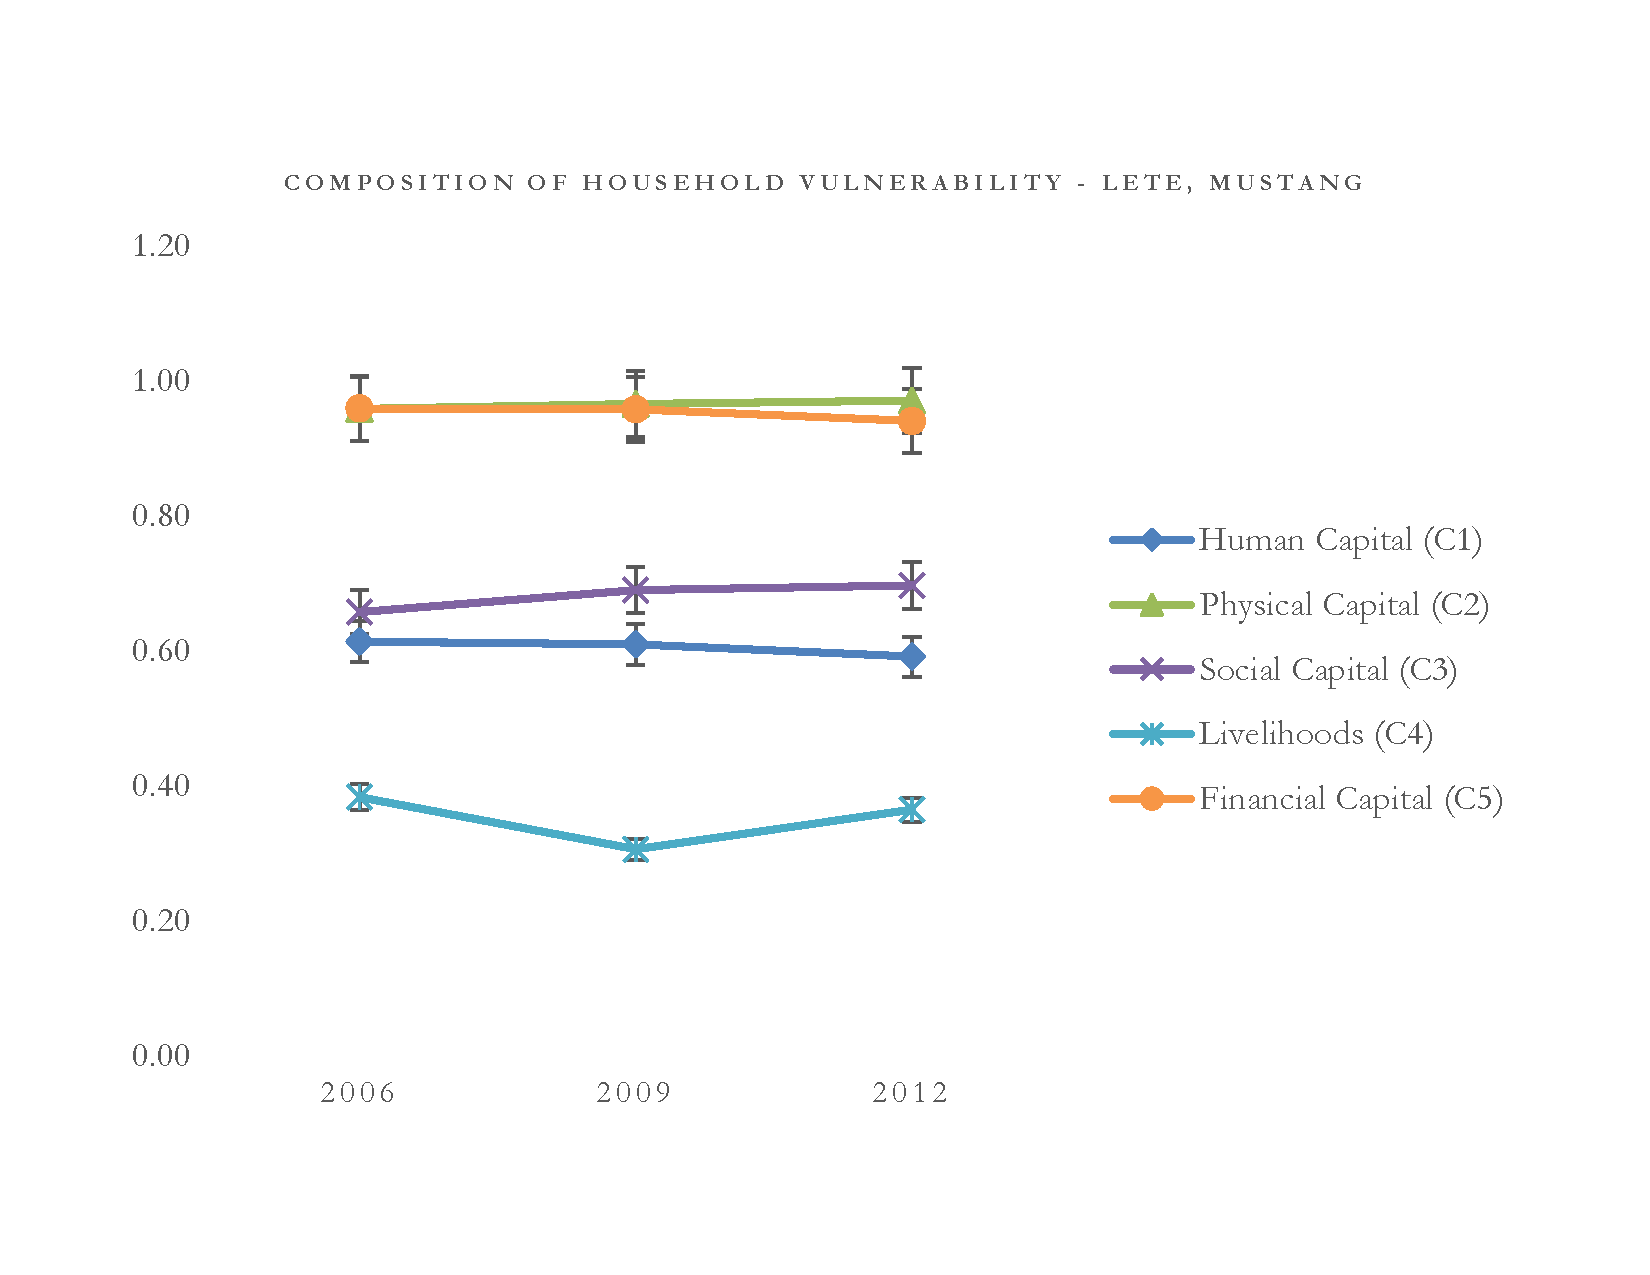
\includegraphics[scale=0.6]{HVI_Component_Lete1.pdf}
	\captionsetup{labelformat=empty}
	\caption{Figure 4.6: Component of HVI - Lete VDC, Mustang}
	\setlength{\abovecaptionskip}{1pt}
	\label{fig:hviletecomponents}
\end{figure}

A panel summary of the components of the HVI is presented in Appendix Table 2. Further a composed stacked line with markers is presented in Appendix Fig 1.

\subsection*{4.5 Persistence and Transience of Household Vulnerability}
\addcontentsline{toc}{subsection}{4.5 Persistence and Transience of Household Vulnerability}
\renewcommand{\thepage}{\arabic{page}}
Figure 4.7 is a Sankey diagram presenting the persistence and transitions of the household vulnerability level across the waves of survey. The value labels represent the number of households that are in the corresponding vulnerability. \\

\begin{figure}[H]
	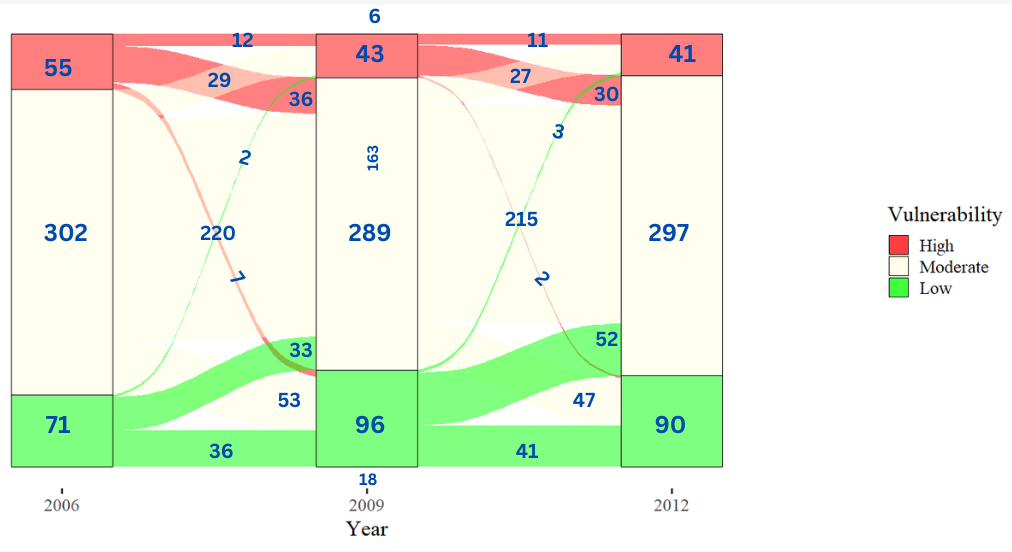
\includegraphics[scale=0.6]{Sankey.png}
	\captionsetup{labelformat=empty}
	\caption{Figure 4.7: Persistence and Transience of Household Vulnerability}
	\setlength{\abovecaptionskip}{2pt}
	\label{fig:hviletecomponents}
\end{figure}

The details of the Vulnerability level across the survey waves (2006, 2009, 2012) is presented in Table 4.9. In the table, in 2006 there are 55 households categorised as "High", 302 as "Moderate" and 71 as "Low" vulnerability level. In 2009, the number of households classified as "High" vulnerability decreased to 43, "Moderate" vulnerability decreased to 289, and "Low" vulnerability increased to 96.
In 2012, the number of households classified as "High" vulnerability further decreased to 41, "Moderate" vulnerability increased slightly to 297, and "Low" vulnerability decreased to 90.

\begin{table}[H]
	\captionsetup{labelformat=empty}
	\captionsetup{labelformat=empty, skip=-7pt} % Adjust the skip to reduce space
	\caption{{Table 4.9}: Vulnerability level across the waves of survey} 	\label{tab:Vulnerabilitylevels} 	\begin{center}
	\begin{tabular}{lccc} \hline
		\textbf{Vulnerability level} & \textbf{2006}            & \textbf{2009}            & \textbf{2012}           \\ \hline
		High                         & 55                       & 43                       & 41                      \\
		Moderate                     & 302                      & 289                      & 297                     \\
		Low                          & 71                       & 96                       & 90                \\ \hline \hline     
	\end{tabular}\\
\end{center}\vspace{-8pt}
\textit{\ \ \ \ \ \ \ \ \ \ \ \ \ \ \  \ \ \ \ \ \ \ \ Source:Author's calculation}
\end{table}

Table 4.10 presents the transition of the vulnerability levels of the households. This table shows the household transitioning from one vulnerability level to another between each pair of survey years. For example, from 2006 to 2009, there were 12 households that were "High" vulnerability in 2006 and remained "High" vulnerability in 2009. Similarly, there were 36 households that were "High" vulnerability in 2006 and transitioned to "Moderate" vulnerability in 2009.

	\begin{table}[H]
	\captionsetup{labelformat=empty}
	\captionsetup{labelformat=empty, skip=-7pt} % Adjust the skip to reduce space
	\caption{{Table 4.10}: Transition matrix of the household vulnerability}
	\label{tab:Vulnerabilitytransitions}	\begin{center}
	\begin{tabular}{lcc} \hline
		\textbf{Vulnerability Level} & \textbf{2006-2009} & \textbf{2009-2012} \\ \hline
		High to High                 & 12                 & 11                 \\
		High to low                  & 7                  & 2                  \\
		High to Moderate             & 36                 & 30                 \\
		Low to High                  & 2                  & 3                  \\
		Low to Low                   & 36                 & 41                 \\
		Low to moderate              & 33                 & 52                 \\
		Moderate to High             & 29                 & 27                 \\
		Moderate to low              & 53                 & 47                 \\
		Moderate to Moderate         & 220                & 215       \\ \hline \hline        
	\end{tabular} \\
	\end{center}\vspace{-8pt}
	\textit{\ \ \ \ \ \ \ \ \ \ \ \ \ \ \ \ \ \ \ Source:Author's calculation}
\end{table}

Table 4.11 presents the persistence of vulnerability across the survey waves. It highlights the number of households that remained in the same vulnerability level throughout the entire period of 2006 to 2012. There were 6 households that remained in the "High" vulnerability category from 2006 to 2012. Similarly, there were 18 households that remained in the "Low" vulnerability category throughout the same period.



\begin{table}[H]
	\captionsetup{labelformat=empty}
	\captionsetup{labelformat=empty, skip=-7pt} % Adjust the skip to reduce space
	\caption{{Table 4.11}: Persistence of vulnerability the household 2006-2009-2012}
	\label{tab:Vulnerabilitypersistence}
	\begin{center}
	\begin{tabular}{lc} \hline
		\textbf{Vulnerability level} & \textbf{No. of Households} \\	\hline
		High to High & 6 \\
		Low to Low            & 18         \\
		Moderate to Moderate  & 163  \\ \hline \hline     
	\end{tabular} \\
	\end{center}\vspace{-8pt}
	\textit{\ \ \ \ \ \ \ \ \ \ \ \ \ \ \ \ \ \ \ \ \ \ Source:Author's calculation}
	\end{table}

\clearpage
\subsection*{4.6 Results from Empirical Analysis}
\addcontentsline{toc}{subsection}{4.6 Results from Empirical Analysis}
\renewcommand{\thepage}{\arabic{page}}
This section presents the results for the household vulnerability regression estimates. We report the marginal effects, standard errors for all the models included in the regression. We included household vulnerability index as an dependent variable which we calculated using equation 3.8. For the independent variable, we used Environmental dependence, Debt, Dependency ratio and Shock as the independent variable. While Environmental income could be an important source of smoothing consumption but could be considered a liability rather than a capital for the vulnerable households.  Our results find that household's vulnerability increases as environmental dependence increases. 

Other factors influencing household vulnerability included Debt. Our results, though insignificant, confirms that debt could reduce the household vulnerability. Also, Dependency ratio was a liability factor of the household's resilience. Our regression results is similar with the findings of the prior literature. The other control we include in the model is the shock as measured by the number of shocks experienced by the households. This study finds that as the the number of shocks increases the household vulnerability increases. Fixed effects controls have also been introduced in the regression models to account for the variation caused by the time-invariant variables such as district and VDC.

Table 4.12 presents the results of the Panel Data regression employed in the analysis. 3 methods of Panel data namely: Pooled OLS; Random Effects; and Fixed Effects have been employed to investigate the factors that affect household vulnerability. The first model is a simple Pooled OLS model where the dependent variable household vulnerability has been regressed by Environmental dependence. The result on the regression is that Environmental dependence increases the household vulnerability. The significance level is on 1\%. This simple regression has been the landmark of this analysis. Following the result, we extend the regression in the following models for Pooled OLS by adding control variables Debt, Dependency ratio and Shock. Further, we add Fixed effects of Year, District and VDC. The result of the step-wise regression is on the Appendix Table 2. The final result of a full specification model of the POLS regression in the Table 4.12 suggests a significantly positive association between household vulnerability and environmental dependence.

\begin{table}[H] 
	\begin{center}
		\captionsetup{labelformat=empty}
	\caption{Table 4.12: Panel Data Regression} 
	\label{} 
	\renewcommand{\arraystretch}{0.9}
	\resizebox{0.9\textwidth}{!}{%
	\begin{tabular}{@{\extracolsep{1pt}}lD{.}{.}{-3} D{.}{.}{-3} D{.}{.}{-3} D{.}{.}{-3} } 
		\\[-2ex]\hline 
		\hline \\[-2.5ex] 
		& \multicolumn{4}{c}{\textit{Dependent variable: Household Vulnerability}} \\ 
		\cline{2-5} \\
		[-2.6ex] & \multicolumn{1}{c}{POLS (1)} & \multicolumn{1}{c}{POLS (2)} & \multicolumn{1}{c}{RE} & \multicolumn{1}{c}{FE}\\ 
		\hline \\[-2.8ex] 
		Env. Dependence & 0.068^{***} & 0.045^{***} & 0.024^{**} & -0.004 \\ 
		& (0.012) & (0.012) & (0.011) & (0.013) \\ 
		& & & & \\ [-1.8ex]
		Debt &  & -0.0005 & -0.0004 & -0.0003 \\ 
		&  & (0.0003) & (0.0003) & (0.0003) \\ 
		& & & & \\ [-1.8ex] 
		Dependency ratio &  & 0.020^{***} & 0.018^{***} & 0.014^{***} \\ 
		&  & (0.002) & (0.002) & (0.002) \\ 
		& & & & \\ [-1.8ex] 
		Shock &  & 0.001 & 0.001 & 0.001 \\ 
		&  & (0.001) & (0.001) & (0.001) \\ 
		& & & & \\ [-1.8ex] 
		Constant & 0.557^{***} & 0.562^{***} & 0.583^{***} &  -  \\ 
		& (0.012) & (0.012) & (0.011) & -  \\ 
		& & & & \\[-2.5ex] 
		\hline \\[-3.3ex] 
		\textit{Fixed Effects} & & & & \\ [-1.5ex]
		Year & \multicolumn{1}{c}{No} & \multicolumn{1}{c}{Yes} & \multicolumn{1}{c}{Yes} & \multicolumn{1}{c}{Yes} \\ [-0.9ex]
		District & \multicolumn{1}{c}{No} & \multicolumn{1}{c}{Yes} & \multicolumn{1}{c}{Yes} & \multicolumn{1}{c}{Yes} \\ [-0.9ex]
		VDC & \multicolumn{1}{c}{No} & \multicolumn{1}{c}{Yes} & \multicolumn{1}{c}{Yes} & \multicolumn{1}{c}{Yes} \\ 
		\hline \\[-3.3ex] 
		\textit{Fit statistics} & & & & \\ [-1.5ex]
		Observations & \multicolumn{1}{c}{1,284} & \multicolumn{1}{c}{1,284} & \multicolumn{1}{c}{1,284} & \multicolumn{1}{c}{1,284} \\ [-0.9ex]
		R$^{2}$ & \multicolumn{1}{c}{0.024} & \multicolumn{1}{c}{0.131} & \multicolumn{1}{c}{0.095} & \multicolumn{1}{c}{0.042} \\[-0.9ex] 
		Adjusted R$^{2}$ & \multicolumn{1}{c}{0.023} & \multicolumn{1}{c}{0.125} & \multicolumn{1}{c}{0.089} & \multicolumn{1}{c}{-0.446} \\ 
		\hline 
		\hline \\ [-2.8ex] 	
		\end{tabular}
	}
\parbox{\linewidth}{\textit{ \ \ \ \ \ Note: Standard errors in the parenthesis:} \ \ \ \ \ {$^{*}$p$<$0.1; $^{**}$p$<$0.05; $^{***}$p$<$0.01}} \\ \vspace{-0.35cm}
\parbox{\linewidth}{\textit{\ \ \ \ \ \ Env. = Environmental}}
 
\end{center}
\end{table}   

After running the Pooled OLS regression we ran the Lagrange Multiplier Test -  \cite{honda1988size} to test if there are time effects in our model. The Null hypothesis is that there are no time effects in the model. The result indicate that there are significant time effects in the model. The test statistic is 10.822 and the p-value is extremely small (0.000) which suggests that there is a strong evidence to reject null hypothesis. The result of the test is in the Appendix B1. 

Similarly, we also tested for the individual effects in the Pooled OLS model. We conducted F-test and found that there are individual effects (fixed effects) in the model. The results suggests strong evidence to reject the null hypothesis. The F-statistics is 2.4874 with degree of freedom df1=472 and df2=852. The p-value is extremely small (0.000). This implies that there are significant individual effects in the model. The results of the tests are in Appendix B2.

Referring to the results of the test, we included the time factor (Year) as well as time-invariant factors District and VDC. Since, the result suggested that there is strong evidence that there are time as well as individual effects. So, we controlled the Year, District and VDC fixed effects.

After obtaining the results from the Pooled OLS regression, we tested for the pool-ability to confirm if the cross-sectional unit in the panel has the same intercept or a different intercept. Also, whether or not it had different slopes. For this purpose, we employed Breusch and Pagan Lagrangian multiplier test \citep{breusch1980lagrange} to test the poolability of the data. It was confirmed that the panel data was not pool-able. So, Pooled OLS is not appropriate for the model. The result of the Breusch and Pagan Lagrange Multiplier test is in Appendix B3.

Since the BP-LM test result indicate that p-value = 0.000, we conclude that the Pooled OLS model is not an efficient estimator for our data. So, we run Random Effects (RE) model. The result of the RE regression is in the Table 4.12 which suggests that there is a positively significant relationship between the household vulnerability and environmental dependence which implies that as the environmental dependency increases the household becomes more vulnerable. The results from the Random Effects (RE) model closely resemble those from the Pooled Ordinary Least Squares (POLS) model. However, there are slight differences in the coefficients and their significance levels between the two. The step-wise regression results for the Random effects (RE) is on the Appendix Table 3. The model progression is similar to Pooled OLS model. The first model is simple Random effects model with dependent variable household vulnerability and only on independent variable environmental dependence. Then in the subsequent models, control variables Debt, Dependency ratio, Shock is added gradually. Furthermore, Fixed effects for Year, District and VDC were considered in the model in the similar fashion. 

We also run the fixed effects (FE) regression. The result of the full specification FE model is in the Table 4.12. It suggests that there is a  negative but non-significant relationship between Environmental dependence and household vulnerability. However, for other control variables, the results are similar to those of Pooled OLS and RE. The step-wise regression for FE is in the appendix Table 4. The model progression is similar to Pooled OLS and RE model. The first model is simple Random effects model with dependent variable household vulnerability and only on independent variable environmental dependence. Then in the subsequent models, control variables Debt, Dependency ratio, Shock is added gradually. Furthermore, Fixed effects for Year, District and VDC were considered in the model in the similar fashion.      
   
After the FE regression, we conduct Hausman Specification test \citep{hausman1978specification}. The test assesses whether the coefficients estimated by the two models are significantly different. The test for our model suggest that fixed effect model is preferred over random effect model. The corresponding chi-square value is 25.48 which is relatively large with 6 degrees of freedom, and the adjoint probability was much less than 0.05. The result obtained for Hausman Specification test is in the Appendix B4.

However, we take the inference of RE as efficient estimates. In random-effects, one of the fundamental assumptions is that the unobserved individual effects, $\mathit{\alpha_i}$, are randomly drawn from the population. In this sense, RE estimator is efficient, consistent and unbiased estimator when T is small and N is large \citep{hsiao2022analysis}. The advantage of random effects inference is that the number of
parameters is fixed when sample size increases. It also allows the derivation of efficient
estimators that make use of both within- and between-group variation. The impact of
time-invariant variables can also be estimated.
\subsection*{4.6.1.1 Environmental Dependence and Vulnerability (OLS)}
Appendix Table 3 presents the results of the Pooled OLS Regression results. The model specification is in equation 3.9. Model 1 of the equation is a bi-variate regression with household vulnerability as an dependent variable and only Environmental dependence as an dependent variable. The result suggest that there is a significantly positive association between the household vulnerability and environmentally dependence. It suggest that as environmental dependence increases for a household, the household vulnerability increases. 

In model 2, we introduce Debt, one of the variables controlled for in our regression model. Debt has a significantly negative effect on household vulnerability. The regression coefficient of Environmental dependence didn't change after the introduction of the control variable debt. 

In the following models 3, 4 we further introduce the control variables Dependency ratio and Shock respectively. The addition of the variables in our model only slightly changed the coefficient of the Environmental dependence. Dependency ratio is shown to have positive effect on household vulnerability in both the models. In the model 4, shock also is exhibited to have a positive and significant influence on household's vulnerability. For the remaining models (5, 6, and 7), Year, District, and VDC fixed effects were introduced consecutively. Even after the Fixed effects were applied, significance and direction of our main independent variable Environmental dependence remained same as the model 1. However, the coefficient were on a declining trend as the control variables were added in the model. The shock variable lost its significant but the direction remained the same, implying that shock has a positive effect on household vulnerability.

The Pooled OLS regression results indicates that that environmental dependence increases the household's vulnerability. Similarly, the increase in the Dependency ratio also increases the household vulnerability. Shock variable also has a positive effect on household vulnerability. However, debt has a negative influence on household vulnerability.  
  
\subsection*{4.6.1.2 Environmental Dependence and Vulnerability (RE)}
Appendix Table 4 presents the Random Effects Regression results of our estimates. The model specification is same as of Pooled OLS Model. Result from Model 1 suggest that there is a significantly positive association between the household vulnerability and environmentally dependence. Here, no control variables have been included.  

Controls such as: Debt; Dependency; and Shock have been included in the following models 2, 3 and 4 respectively. Debt, in the model 2 had a significantly negative effect on household's vulnerability, indicating that the debt reduces the household vulnerability. However, it lost its significance in the model 3 following the addition of dependency ratio in the model. The direction remained unchanged nonetheless. In model 4, dependency ratio and shock had a positive effect on household vulnerability.

Similarly, in the models 5 , 6 and 7, random effects regression were run with Year, District and VDC fixed effects in the consecutive models. In model 5, with the Year fixed effects, Debt had a negative but insignificant effect on household vulnerability. Dependency ratio had a positive and significant effect on household vulnerability. Shock variable had a positive but insignificant effect on the dependent variable in the model. The same trend is observed across the following models. 

Importantly, our major variable of interest Environmental dependence continued to have a positive effect across all the models.  Up to model 5, Environmental dependence displayed to have a positive effect on household vulnerability at 1\% significance level. However, the significance level reduced to 5\% in the following models. The loss in the significance is the effect of introduction of the time invariant fixed effects: District and VDC.

\subsection*{4.6.1.3 Environmental Dependence and Vulnerability (FE)}
Appendix Table 5 presents the regression estimates of Fixed effects model. The model specification is same as of Pooled OLS Model and Random Effects Model. Result from Model 1 suggest that there is a negative association between the household vulnerability and environmentally dependence. However, there is no significance of the effect. Here, no control variables have been included.  

Controls such as: Debt; Dependency; and Shock have been included in the following models 2, 3 and 4 respectively. Debt, in the model 2 also had a negative effect on household's vulnerability, indicating that the debt reduces the household vulnerability. The effect is not significance nevertheless. The direction has remained unchanged. In model 3 and 4, dependency ratio had a significantly positive effect on household vulnerability. The coefficient and significance is consistent in model 5. Shock in the model 4 had a positive and significant effect on household vulnerability. 

In models 5, 6, and 7, Fixed Effects Regression was employed, incorporating Year, District, and VDC fixed effects in successive iterations. In model 5, the inclusion of Year fixed effects revealed a negative but statistically insignificant impact of Debt on household vulnerability. Conversely, the Dependency ratio exhibited a positive and statistically significant association with household vulnerability. The Shock variable displayed a positive yet statistically insignificant effect on the dependent variable in this model. This pattern persisted consistently in the subsequent models.

Environmental dependence, consistently demonstrated a negative and insignificant effect upto model 6. However, in the model 7, the effect was positive and significant. This implies that the best fit of the model is when all the relevant and necessary variables are included in the model. 

\subsection*{4.7 Discussion}
\addcontentsline{toc}{subsection}{4.7 Discussion}
\renewcommand{\thepage}{\arabic{page}}
\setstretch{1.5}
\subsection*{4.7.1 Household Vulnerability Index}
With the objective of assessment of household vulnerability in the three distinct physio-graphical region: Mountain; Mid-hill; and Lowland region of Nepal, we constructed household vulnerability index for the Kunjo and Lete VDC of Mustang, Hemja VDC of Kaski and Chainpur VDC of Chitwan. We employed the Min-Max standardization in 3.5 to 3.8 for standardizing the values of the variables in order to construct the HVI. 

From the HVI, we find that HVI ranged from 0.61 to 0.65 across the survey districts in the year 2006. Kunjo and Lete of Mustang district had the highest vulnerability in the year 2006. These VDCs persisted to be the most vulnerable across all waves of the survey years. It can be inferred from this that mountainous region still the most vulnerable of all. Mountainous regions of Nepal are often characterized by geographical and infrastructural difficulties which hinders the region of the opportunities. The resources in the region are scarce and unevenly distributed leading to heightened socio-economic disparities.    


Contrary to mountain, Hill and Lowland region enjoys more resources and infrastructural advantages. So, the HVI for these regions are less than that of Mountains.  Hemja VDC of Kaski persisted on a same level of vulnerability with 0.62. By 2012, mild changes were observed, with certain VDCs experienced lowered vulnerability across the waves of survey. Chainpur VDC of Chitwan experienced a slight decrease in vulnerability from 2006 to 2009 but the level persisted in the year 2012. Kunjo VDC of Mustang followed a similar trend.  

We presented the District level as well as VDC level HVI in the radar chart in Fig 4.1 and 4.2. Similarly, we also present the Component of household vulnerability index in a stacked line with markers for each VDCs across all rounds of survey years in Figure 4.3, 4.4, 4.5 and 4.6. The persistence and transience of the vulnerability positions of each VDCs in each village is presented in a Sankey diagram in Fig 4.7.
 

 \subsection*{4.7.2 Household Vulnerability and Environmental Dependence}  
After the assessment of the vulnerability positions of the VDCs and Districts across the survey years, we carry out the empirical estimation to find the relationship between the household vulnerability and environmental dependence. For that purpose, we carry out Panel data regression employing Pooled OLS, Random Effects (RE) and Fixed Effects (FE) regression techniques. The dependent variable is household vulnerability as measured by HVI and the independent variables include Environmental dependence, Debt, Dependency ratio, Shock. Other controls are Year, District and VDC fixed effects. Yeas as a time fixed effects and District and VDC as time-invariant fixed effects were added in the model 5-7. It had its effect in changing the coefficients of the variables. 

\cite{angelsen2015environmental, abbas2018sustainable, gentle2014differential} contests that environmental resource dependence had a positive effect on household vulnerability, particularly in the context of changing climate and climatic hazards. Our result confirms the findings of the literatures. Appendix Table 3, 4 and 5 presents the results of the Pooled OLS, Random Effects and Fixed Effects regression respectively. A total of 7 models have been included in the regression. based on the literature. Model 1 is a bi-variate regression whose result show that there is a significant positive relationship between Environmental dependence and household vulnerability. Model 2 to model 4 are multi-variate regression models where additional controls are added in the model consecutively. The addition of the controls in the model didn't alter the significance and direction of the effect of the Environmental dependence on household vulnerability. 

In the survey districts, households rely on environmental resources for their livelihoods. The reliance is more for those households with low income and less diversified livelihood \citep{walelign2020environmental}. However, this dependence can exacerbate household vulnerability by increasing sensitivity to climate change, limited diversification of livelihood sources, increased resource degradation, exposure to extreme idiosyncratic and co-variate shocks.

Debt is one of the coping mechanisms of the household, particularly when faced with some sort of shock \citep{rabbani2021role}. It plays an important role in reducing the household vulnerability by providing financial resources to cope with shocks and invest in resilience-building measure. Debt not only plays a role of cushion against shocks but also as a source of investment for productive activities, expenditure in education and healthcare, builds the capitals such as physical, financial and social capital. The result of the empirical analysis suggests that debt has a negative effect on household vulnerability, implying that it helps to reduces the vulnerability.



Having more dependent in the household increases the vulnerability of the household \citep{rabbani2021role, sun2020nexus}. A high dependency ratio is characterized by financial strain, reduced labor productivity, limited social support, and inter-generational transmission of poverty.  The empirical results of our study suggest that dependency ratio had a significantly positive influence on household vulnerability.


Number of studies including \cite{buhler2018shocks, barua2020impact, volker2010rural} show that the shocks can push the household to be vulnerable. Shocks increase household vulnerability by disrupting livelihoods, depleting assets, exacerbating food insecurity and malnutrition, imposing health impacts and healthcare costs, causing psychological trauma, etc. The results of our study also suggest that shock had a positive influence in all of the models.

Overall, this thesis study finds that environmental dependence is able to positively influence household vulnerability. Similarly dependency ratio and shock variables are able also had a positive effect on household vulnerability. Debt had a negative effect on household vulnerability.   
 
  
   
            
\clearpage
\begin{center}
\section*{\large{CHAPTER V \\ \vspace{-0.3cm} SUMMARY AND CONCLUSIONS}}
\end{center}
\addcontentsline{toc}{section}{\textbf{CHAPTER V:  CONCLUSION AND RECOMMENDATIONS }}
\renewcommand{\thepage}{\arabic{page}}
\setstretch{1.5}
In this chapter, the summary of the study is presented in the first section. The conclusion, recommendations, and potential extensions are shown in the subsequent
section. \\
\subsection*{5.1 Summary of the Findings}
\addcontentsline{toc}{subsection}{5.1 Summary of the Findings}
\renewcommand{\thepage}{\arabic{page}}
\setstretch{1.5}
The central focus of this thesis is the comprehensive analysis of household vulnerability in rural Nepal. The research aims to delve into the inter-temporal dynamics of vulnerability and conduct a physio-graphic analysis by constructing a household vulnerability index (HVI). The HVI is developed by integrating various capitals, including Human capital, Physical capital, Financial capital, Livelihood strategies, and Social capital. Additionally, the study explores the factors influencing household vulnerability in the context of rural Nepalese households.

The research employs a unique and environmental augmented household-level livelihood panel data-set, as outlined in \citep{walelign2022unique}. This data-set spans the period from 2006 to 2012 and is sourced from Tribhuvan University’s Institute of Forestry and the University of Copenhagen’s Department of Food and Resource Economics. The data-set serves as a valuable resource for capturing the nuances of household livelihoods over time. 

The construction of the household vulnerability Index is a pivotal aspect of the research methodology, accomplished through the application of Mini-max and Maxi-min methods. These methods enable a comprehensive assessment of vulnerability by considering multiple dimensions. The analysis of the household vulnerability reveals distinct patterns. Chitwan exhibits a slightly variable vulnerability level with a mean household vulnerability index (HVI) of 0.62 in 2006, and 0.61 in 2009 and 2012. Kaski shows stable vulenrability, of 0.62 across 2006, 2009 and 2012. Mustang indicates higher vulnerability in 2006 (0.64), a slight decrease in 2009 (0.63), and stability in 2012.  Radar charts further depict the variability within districts, with Kaski's polygon suggesting consistent vulnerability, Chitwan's indicating at potential decrease, and Mustang's showing fluctuations followed by stabilization.  

Furthermore, the study employs Panel Data Regression techniques, including Pooled Ordinary Least Squares (OLS), Fixed Effects (FE), and Random Effects (RE) regression, to identify and quantify the factors influencing household vulnerability. Notably, environmental dependence emerges as a key contributor to increased household vulnerability in the rural households.

The study reveals a positive association between dependency ratios and the household vulnerability Index (HVI), indicating that a higher dependency ratio exacerbates vulnerability. Additionally, the analysis suggests that shocks to households also play a substantial role in elevating vulnerability levels. The research finds a mitigating effect of debt on household vulnerability, suggesting that households with certain debt levels exhibit lower levels of vulnerability. 


\subsection*{5.2 Conclusion}
\addcontentsline{toc}{subsection}{5.2 Conclusion}
\renewcommand{\thepage}{\arabic{page}}
\setstretch{1.5}
The research examines the relationship between the household vulnerability and environmental dependence in the rural households across the physio-graphic regions utilizing various capital such as Human Capital, Physical Capital, Social Capital, Financial Capital and Livelihood. A composite index was developed using the mini-max normalization method. The index allowed the analysis of the vulnerability on a household, village and district level. 

From the analysis, we found that Chitwan district had a stable vulnerability across all waves of the survey (2006, 2009, 2012) with a mean HVI of 0.61. Kaski district exhibited mild variability, with a decrease in mean HVI from 2006 to 2009 and an increase back to the original level in 2012.
Mustang district showed relatively higher household vulnerability in 2006, a slight decrease in 2009, and stability in 2012. 

After the household vulnerability analysis, we investigated its relationship with Environmental Dependence. The household vulnerability index, calculated based on established equations, served as the dependent variable. Environmental dependence as a major determinant, consistently exhibited a significantly positive association with vulnerability. If the dependence persists further, it might have an adverse effect on the households as well as the environment. Household vulnerability increases because they are prone to environmental risk. From the environmental perspective, this dependence is a threat to sustainable environment as it will degrade the environment.

Additionally, the study attempted to study the association of Debt on vulnerability. Debt, as a coping mechanism, displayed a negative relationship with vulnerability, though statistically insignificant. Debt plays important role of reducing vulnerability of the households in multi-faceted manner. It acts as a safety nets during the times of shocks and crisis by providing immediate financial support. It also enables households to invest in productive activities which reduces vulnerability and increases resilience capacity of the households in the long-run. Further, it helps to strengthen the capitals of the households that make the household resilient. Capitals such as Financial and Social Capital.  

A high dependency ratio is characterized by a large proportion of dependents relative to the working-age population. A high dependency ratio has a positive effect on household vulnerability. Having a high dependency ratio leads to heightened vulnerability to economic shocks and poverty, perpetual cycles of financial instability and deprivation. Having higher number of elderly and children means that the adult working age family member needs to refrain from participating in the labor force in order to do the care work for the dependents. This in turn exacerbates the vulnerability of the households. 

Households in rural Nepal face a lot of shocks that impact their livelihoods severely. Natural disasters, economic downturns, or health shocks or any other idiosyncratic or co-variate shocks increase the vulnerability of the household. Moreover, shocks exacerbate pre-existing vulnerabilities, disproportionately affecting poor and vulnerable. Shocks have a multifaceted influence on the household and vulnerability. The result of the study confirms that households facing more number of shocks are more vulnerable. 

\subsection*{5.3 Recommendations and Possible Extensions}
\addcontentsline{toc}{subsection}{5.3 Recommendations  and Possible Extensions}
\renewcommand{\thepage}{\arabic{page}}
\setstretch{1.5}
This thesis builds national and sub-national level vulnerability assessment \cite{antwi2013characterising, aksha2019analysis, shahiestimating} by developing and applying a household vulnerability index to characterize the nature and inter-temporal dynamics of the household vulnerability across the distinct geographic regions of Nepal. This study targets an important gap in the literature, improving understanding of the processes and factors that affect vulnerability, with a view to guiding the development of effective policies. The findings and result has shown that across the distinct geographical setting, different communities and households may experience differential vulnerability that may be attributed to differences in capitals possessed by the households. The analysis showed that across the rural setting communities, Mountainous village of Mustang district had a relatively higher household vulnerability. 

This contrast between the Nepal's diverse geographic landscape, significantly influences rural livelihoods and prevalence of subsistence economies. These differences must be taken into account when drafting the interventions to address specific vulnerabilities in areas exhibiting different patterns. Further, it is important to prioritize the environmental factors and household's dependency on environment. This thesis finds that there is a positive relationship between Environmental dependency and household vulnerability. So, policies that attempt to lower the dependency on the environment must be designed and implemented in rural setting. Additionally, community-level resilience programs, educational initiatives, and cross-sectoral collaboration could be proposed to address the multifaceted nature of household vulnerability.  These programs and policies may help to foster sustainable development, resilience, and improved livelihoods in rural Nepalese communities while accounting for the specific geographical and economic characteristics of each region. 

Further, there is a need to leverage debt to reduce the vulnerability. The households should be facilitate to invest the funds from the debt in productive assets, education, healthcare, and social capital to enhance resilience and income-generating opportunities. Alongside, household needs to practice responsible borrowing and effective debt management strategies to prevent excessive indebtedness and financial instability. Policies should be aimed at enhancing access to credit and financial services for the vulnerable households to facilitate economic empowerment and resilience-building initiatives.

In part of dependency ratio, there needs to be a social safety nets to provide services to the dependent population so that the financial strain on household with higher dependency ratio could be alleviated to some extent. Further, care facilities needs to be available in communities so that the working age population could participate in the labor force, without worrying about the dependent family members in the house. 

Also to mitigate the vulnerability to shocks, policies should be aimed at providing adequate safety nets and designing welfare programs to provide immediate relief and support to the vulnerable households affected by the shocks. Government needs to investments in disaster preparedness, risk reduction, and resilient infrastructure. This will ensure quick relief as well as the recovery.   

Moreover, there is a possibility for this version of the study to be expanded. Due to time and resource constraints, we used the equal weighting approach at the time of computing the household vulnerability index. In future studies, consultation with stakeholders regarding the weight of the the components of the household vulnerability could be discussed and apply the weights.

          
\clearpage

	
\bibliographystyle{apacite}
\setlength{\bibsep}{0pt}
\setlength{\bibhang}{4em}
\renewcommand{\bibname}{\centering\large\MakeUppercase{References}}
\bibliography{bibliography}
\renewcommand{\thepage}{\arabic{page}}
\clearpage

\begin{center}
\section*{APPENDICES}
\end{center}
\addcontentsline{toc}{section}{\textbf{APPENDICES }}
\renewcommand{\thepage}{\arabic{page}}

\begin{landscape}
\begin{table}[ht]
	\caption*{Appendix Table 1: VDC-wise variables used for the construction of Household Vulnerability Index}
	\renewcommand{\arraystretch}{1.2}
	\resizebox{1.8\textwidth}{!}{%
		\begin{tabular}{lcccccccccccc}
			\hline
			\multirow{3}{*}{\textbf{\begin{tabular}[c]{@{}l@{}}Year/\\ District/\\ VDC\end{tabular}}} & \multicolumn{4}{c}{\textbf{2006}}                                                                                                                                                                                                                               & \multicolumn{4}{c}{\textbf{2009}}                                                                                                                                                                                                                               & \multicolumn{4}{c}{\textbf{2012}}                                                                                                                                                                                                                               \\ \hline
			& \textbf{Chitwan}                                              & \textbf{Kaski}                                                & \multicolumn{2}{c}{\textbf{Mustang}}                                                                                            & \textbf{Chitwan}                                              & \textbf{Kaski}                                                & \multicolumn{2}{c}{\textbf{Mustang}}                                                                                            & \textbf{Chitwan}                                              & \textbf{Kaski}                                                & \multicolumn{2}{c}{\textbf{Mustang}}                                                                                            \\ \hline
			& \textbf{Chainpur}                                             & \textbf{Hemja}                                                & \textbf{Kunjo}                                                 & \textbf{Lete}                                                  & \textbf{Chainpur}                                             & \textbf{Hemja}                                                & \textbf{Kunjo}                                                 & \textbf{Lete}                                                  & \textbf{Chainpur}                                             & \textbf{Hemja}                                                & \textbf{Kunjo}                                                 & \textbf{Lete}                                                  \\ \hline
			\multicolumn{13}{l}{\textbf{Human Capital}}                                                                                                                                                                                                                                                                                                                                                                                                                                                                                                                                                                                                                                                                                                                                                                                                                                                     \\
			HHH Age                                                                                   & \begin{tabular}[c]{@{}c@{}}50.36\\  (14.15)\end{tabular}      & \begin{tabular}[c]{@{}c@{}}50.14 \\ (14.57)\end{tabular}      & \begin{tabular}[c]{@{}c@{}}51.54\\  (14.66)\end{tabular}       & \begin{tabular}[c]{@{}c@{}}54.16 \\ (12.32)\end{tabular}       & \begin{tabular}[c]{@{}c@{}}52.13 \\ (13.75)\end{tabular}      & \begin{tabular}[c]{@{}c@{}}52.00 \\ (13.39)\end{tabular}      & \begin{tabular}[c]{@{}c@{}}52.63\\ (14.57)\end{tabular}        & \begin{tabular}[c]{@{}c@{}}55.50\\ (12.95)\end{tabular}        & \begin{tabular}[c]{@{}c@{}}52.24\\ (17.20)\end{tabular}       & \begin{tabular}[c]{@{}c@{}}53.52\\ (13.71)\end{tabular}       & \begin{tabular}[c]{@{}c@{}}52.77\\ (15.92)\end{tabular}        & \begin{tabular}[c]{@{}c@{}}57.54\\ (11.98)\end{tabular}        \\
			HH head Education                                                                         & \begin{tabular}[c]{@{}c@{}}3.08\\ (4.06)\end{tabular}         & \begin{tabular}[c]{@{}c@{}}6.29\\ (4.97)\end{tabular}         & \begin{tabular}[c]{@{}c@{}}2.83\\ (3.42)\end{tabular}          & \begin{tabular}[c]{@{}c@{}}3.25\\ (4.46)\end{tabular}          & \begin{tabular}[c]{@{}c@{}}2.93\\ (4.06)\end{tabular}         & \begin{tabular}[c]{@{}c@{}}6.07\\ (5.23)\end{tabular}         & \begin{tabular}[c]{@{}c@{}}2.79\\ (3.28)\end{tabular}          & \begin{tabular}[c]{@{}c@{}}3.08\\ (4.21)\end{tabular}          & \begin{tabular}[c]{@{}c@{}}2.91\\ (4.33)\end{tabular}         & \begin{tabular}[c]{@{}c@{}}6.91\\ (5.07)\end{tabular}         & \begin{tabular}[c]{@{}c@{}}2.48\\ (3.39)\end{tabular}          & \begin{tabular}[c]{@{}c@{}}3.30\\ (4.62)\end{tabular}          \\
			Max HH Education                                                                          & \begin{tabular}[c]{@{}c@{}}8.44\\ (3.91)\end{tabular}         & \begin{tabular}[c]{@{}c@{}}10.76\\ (2.90)\end{tabular}        & \begin{tabular}[c]{@{}c@{}}7.10\\ (2.92)\end{tabular}          & \begin{tabular}[c]{@{}c@{}}8.14\\ (3.60)\end{tabular}          & \begin{tabular}[c]{@{}c@{}}9.70\\ (3.63)\end{tabular}         & \begin{tabular}[c]{@{}c@{}}11.18\\ (3.94)\end{tabular}        & \begin{tabular}[c]{@{}c@{}}7.75\\ (3.47)\end{tabular}          & \begin{tabular}[c]{@{}c@{}}8.32\\ (4.33)\end{tabular}          & \begin{tabular}[c]{@{}c@{}}9.89\\ (4.44)\end{tabular}         & \begin{tabular}[c]{@{}c@{}}11.91\\ (4.03)\end{tabular}        & \begin{tabular}[c]{@{}c@{}}7.72\\ (3.71)\end{tabular}          & \begin{tabular}[c]{@{}c@{}}8.70\\ (3.97)\end{tabular}          \\
			\multicolumn{13}{l}{\textbf{Physical Capital}}                                                                                                                                                                                                                                                                                                                                                                                                                                                                                                                                                                                                                                                                                                                                                                                                                                                  \\
			Total Implements                                                                          & \begin{tabular}[c]{@{}c@{}}4660.32\\ (11275.49)\end{tabular}  & \begin{tabular}[c]{@{}c@{}}14057.03\\ (16860.42)\end{tabular} & \begin{tabular}[c]{@{}c@{}}6579.07\\ (11240.12)\end{tabular}   & \begin{tabular}[c]{@{}c@{}}13892.80\\ (24616.53)\end{tabular}  & \begin{tabular}[c]{@{}c@{}}10153.80\\ (23970.94)\end{tabular} & \begin{tabular}[c]{@{}c@{}}30700.02\\ (46128.36)\end{tabular} & \begin{tabular}[c]{@{}c@{}}11694.79\\ (16393.21)\end{tabular}  & \begin{tabular}[c]{@{}c@{}}18349.19\\ (31531.21)\end{tabular}  & \begin{tabular}[c]{@{}c@{}}22165.29\\ (38089.25)\end{tabular} & \begin{tabular}[c]{@{}c@{}}48959.02\\ (70582.56)\end{tabular} & \begin{tabular}[c]{@{}c@{}}19824.44\\ (30068.34)\end{tabular}  & \begin{tabular}[c]{@{}c@{}}23000.68\\ (25109.33)\end{tabular}  \\
			Total Livestock                                                                           & \begin{tabular}[c]{@{}c@{}}18532.68\\ (15428.31)\end{tabular} & \begin{tabular}[c]{@{}c@{}}26573.08\\ (20411.58)\end{tabular} & \begin{tabular}[c]{@{}c@{}}64484.18\\ (217769.73)\end{tabular} & \begin{tabular}[c]{@{}c@{}}95156.95\\ (230659.93)\end{tabular} & \begin{tabular}[c]{@{}c@{}}43936.83\\ (39679.84)\end{tabular} & \begin{tabular}[c]{@{}c@{}}35690.11\\ (35760.07)\end{tabular} & \begin{tabular}[c]{@{}c@{}}48328.19\\ (157785.27)\end{tabular} & \begin{tabular}[c]{@{}c@{}}63305.51\\ (196365.44)\end{tabular} & \begin{tabular}[c]{@{}c@{}}38993.71\\ (34330.40)\end{tabular} & \begin{tabular}[c]{@{}c@{}}34635.84\\ (39306.60)\end{tabular} & \begin{tabular}[c]{@{}c@{}}43044.51\\ (40803.87)\end{tabular}  & \begin{tabular}[c]{@{}c@{}}25772.02\\ (36222.90)\end{tabular}  \\
			Total Land owned\\
			(in sq. m)                                                               & \begin{tabular}[c]{@{}c@{}}2027.47\\ (6367.27)\end{tabular}   & \begin{tabular}[c]{@{}c@{}}1187.00\\ (1013.02)\end{tabular}   & \begin{tabular}[c]{@{}c@{}}2851.25\\ (2588.66)\end{tabular}    & \begin{tabular}[c]{@{}c@{}}3023.66\\ (2979.45)\end{tabular}    & \begin{tabular}[c]{@{}c@{}}915.91\\ (765.38)\end{tabular}     & \begin{tabular}[c]{@{}c@{}}1491.41\\ (2060.25)\end{tabular}   & \begin{tabular}[c]{@{}c@{}}2443.77\\ (4381.85)\end{tabular}    & \begin{tabular}[c]{@{}c@{}}2040.13\\ (3034.05)\end{tabular}    & \begin{tabular}[c]{@{}c@{}}1041.46\\ (1136.88)\end{tabular}   & \begin{tabular}[c]{@{}c@{}}1374.96\\ (2253.95)\end{tabular}   & \begin{tabular}[c]{@{}c@{}}2120.03\\ (1955.97)\end{tabular}    & \begin{tabular}[c]{@{}c@{}}1734.96\\ (1825.09)\end{tabular}    \\
			\multicolumn{13}{l}{\textbf{Social Capital}}                                                                                                                                                                                                                                                                                                                                                                                                                                                                                                                                                                                                                                                                                                                                                                                                                                                    \\
			HH belong to \\ biggest caste                                                                & \begin{tabular}[c]{@{}c@{}}0.58\\ (0.50)\end{tabular}         & \begin{tabular}[c]{@{}c@{}}0.89\\ (0.32)\end{tabular}         & \begin{tabular}[c]{@{}c@{}}0.44\\ (0.50)\end{tabular}          & \begin{tabular}[c]{@{}c@{}}0.54\\ (0.50)\end{tabular}          & \begin{tabular}[c]{@{}c@{}}0.66\\ (0.48)\end{tabular}         & \begin{tabular}[c]{@{}c@{}}0.98\\ (0.14)\end{tabular}         & \begin{tabular}[c]{@{}c@{}}0.52\\ (0.50)\end{tabular}          & \begin{tabular}[c]{@{}c@{}}0.63\\ (0.49)\end{tabular}          & \begin{tabular}[c]{@{}c@{}}0.50\\ (0.50)\end{tabular}         & \begin{tabular}[c]{@{}c@{}}0.86\\ (0.50)\end{tabular}         & \begin{tabular}[c]{@{}c@{}}0.50\\ (0.35)\end{tabular}          & \begin{tabular}[c]{@{}c@{}}0.68\\ (0.47)\end{tabular}          \\
			\multicolumn{13}{l}{\textbf{Financial Capital}}                                                                                                                                                                                                                                                                                                                                                                                                                                                                                                                                                                                                                                                                                                                                                                                                                                                 \\
			Bank Saving                                                                               & \begin{tabular}[c]{@{}c@{}}879.58\\ (2661.50)\end{tabular}    & \begin{tabular}[c]{@{}c@{}}9663.83\\ (26812.62)\end{tabular}  & \begin{tabular}[c]{@{}c@{}}26550.42\\ (49925.24)\end{tabular}  & \begin{tabular}[c]{@{}c@{}}36893.08\\ (100295.99)\end{tabular} & \begin{tabular}[c]{@{}c@{}}1911.63\\ (6126.69)\end{tabular}   & \begin{tabular}[c]{@{}c@{}}11937.72\\ (31025.90)\end{tabular} & \begin{tabular}[c]{@{}c@{}}15583.53\\ (33746.90)\end{tabular}  & \begin{tabular}[c]{@{}c@{}}32899.60\\ (75131.34)\end{tabular}  & \begin{tabular}[c]{@{}c@{}}11953.55\\ (31763.88)\end{tabular} & \begin{tabular}[c]{@{}c@{}}25410.64\\ (66932.34)\end{tabular} & \begin{tabular}[c]{@{}c@{}}24116.56\\ (64770.84)\end{tabular}  & \begin{tabular}[c]{@{}c@{}}70411.25\\ (127638.23)\end{tabular} \\
			Jewellery                                                                                 & \begin{tabular}[c]{@{}c@{}}0.00\\ (0.00)\end{tabular}         & \begin{tabular}[c]{@{}c@{}}0.00\\ (0.00)\end{tabular}         & \begin{tabular}[c]{@{}c@{}}17329.52\\ (31072.47)\end{tabular}  & \begin{tabular}[c]{@{}c@{}}45053.31\\ (87655.54)\end{tabular}  & \begin{tabular}[c]{@{}c@{}}4396.88\\ (6965.53)\end{tabular}   & \begin{tabular}[c]{@{}c@{}}20485.87\\ (16594.26)\end{tabular} & \begin{tabular}[c]{@{}c@{}}25209.19\\ (56538.65)\end{tabular}  & \begin{tabular}[c]{@{}c@{}}51106.62\\ (94727.93)\end{tabular}  & \begin{tabular}[c]{@{}c@{}}21477.20\\ (23620.47)\end{tabular} & \begin{tabular}[c]{@{}c@{}}51605.94\\ (48463.62)\end{tabular} & \begin{tabular}[c]{@{}c@{}}45374.61\\ (120899.24)\end{tabular} & \begin{tabular}[c]{@{}c@{}}62313.92\\ (103824.98)\end{tabular} \\
			\textbf{Livelihood}                                                                       & \multicolumn{1}{l}{}                                          & \multicolumn{1}{l}{}                                          & \multicolumn{1}{l}{}                                           & \multicolumn{1}{l}{}                                           & \multicolumn{1}{l}{}                                          & \multicolumn{1}{l}{}                                          & \multicolumn{1}{l}{}                                           & \multicolumn{1}{l}{}                                           & \multicolumn{1}{l}{}                                          & \multicolumn{1}{l}{}                                          & \multicolumn{1}{l}{}                                           & \multicolumn{1}{l}{}                                           \\
			No. of livelihood strategies                                                              & \begin{tabular}[c]{@{}c@{}}4.81\\ (0.97)\end{tabular}         & \begin{tabular}[c]{@{}c@{}}4.72\\ (0.91)\end{tabular}         & \begin{tabular}[c]{@{}c@{}}4.80\\ (0.92)\end{tabular}          & \begin{tabular}[c]{@{}c@{}}4.32\\ (0.93)\end{tabular}          & \begin{tabular}[c]{@{}c@{}}4.93\\ (1.02)\end{tabular}         & \begin{tabular}[c]{@{}c@{}}4.74\\ (0.91)\end{tabular}         & \begin{tabular}[c]{@{}c@{}}5.35\\ (0.83)\end{tabular}          & \begin{tabular}[c]{@{}c@{}}4.86\\ (0.86)\end{tabular}          & \begin{tabular}[c]{@{}c@{}}4.60\\ (0.98)\end{tabular}         & \begin{tabular}[c]{@{}c@{}}4.78\\ (0.90)\end{tabular}         & \begin{tabular}[c]{@{}c@{}}4.76\\ (0.87)\end{tabular}          & \begin{tabular}[c]{@{}c@{}}4.45\\ (1.10)\end{tabular}          \\
			\textbf{Household Vulnerability}                                                          &                                                               &                                                               &                                                                &                                                                &                                                               &                                                               &                                                                &                                                                &                                                               &                                                               &                                                                &                                                                \\
			HVI                                                                                       & \begin{tabular}[c]{@{}c@{}}0.62\\ (0.05)\end{tabular}         & \begin{tabular}[c]{@{}c@{}}0.62\\ (0.04)\end{tabular}         & \begin{tabular}[c]{@{}c@{}}0.65\\ (0.05)\end{tabular}          & \begin{tabular}[c]{@{}c@{}}0.63\\ (0.05)\end{tabular}          & \begin{tabular}[c]{@{}c@{}}0.61\\ (0.05)\end{tabular}         & \begin{tabular}[c]{@{}c@{}}0.62\\ (0.04)\end{tabular}         & \begin{tabular}[c]{@{}c@{}}0.64\\ (0.05)\end{tabular}          & \begin{tabular}[c]{@{}c@{}}0.63\\ (0.05)\end{tabular}          & \begin{tabular}[c]{@{}c@{}}0.61\\ (0.05)\end{tabular}         & \begin{tabular}[c]{@{}c@{}}0.62\\ (0.05)\end{tabular}         & \begin{tabular}[c]{@{}c@{}}0.64\\ (0.05)\end{tabular}          & \begin{tabular}[c]{@{}c@{}}0.62\\ (0.05)\end{tabular}       \\  \hline \hline
		\end{tabular}
	}
	\textit{Note: Standard deviation in the parenthesis \\
	Source: Author's calculation}
\end{table}
\end{landscape}

\begin{landscape}
\begin{center}
	\begin{table}[ht]
		\captionsetup{labelformat=empty}
		\caption*{Appendix Table 2: Mean and SD of the Components used in HVI Construction}
		\label{tab:MeanandSDofComponentsusedinHVIConstruction}
		\resizebox{1.7\textwidth}{!}{%
			\begin{tabular}{lcccccccccccc} \hline
				& \multicolumn{4}{c}{\textbf{2006}}                                                                                                                                                                                                                    & \multicolumn{4}{c}{\textbf{2009}}                                                                                                                                                                                             & \multicolumn{4}{c}{\textbf{2012}}                                                                                                                                                                                             \\ \hline
				& \textbf{Chitwan}                                                             & \textbf{Kaski}                                        & \multicolumn{2}{c}{\textbf{Mustang}}                                                                          & \textbf{Chitwan}                                      & \textbf{Kaski}                                        & \multicolumn{2}{c}{\textbf{Mustang}}                                                                          & \textbf{Chitwan}                                      & \textbf{Kaski}                                        & \multicolumn{2}{c}{\textbf{Mustang}}                                                                          \\ \hline
				\multirow{-3}{*}{\textbf{\begin{tabular}[c]{@{}c@{}}Year/\\ District/\\ VDC\end{tabular}}} & \textbf{Chainpur}                                                            & \textbf{Hemja}                                        & \textbf{Kunjo}                                        & \textbf{Lete}                                         & \textbf{Chainpur}                                     & \textbf{Hemja}                                        & \textbf{Kunjo}                                        & \textbf{Lete}                                         & \textbf{Chainpur}                                     & \textbf{Hemja}                                        & \textbf{Kunjo}                                        & \textbf{Lete}                                         \\ \hline
				\textbf{\begin{tabular}[c]{@{}c@{}}Human Capital (C1)\end{tabular}}                     & \begin{tabular}[c]{@{}c@{}}0.48\\ (0.11)\end{tabular}                        & \begin{tabular}[c]{@{}c@{}}0.49\\ (0.11)\end{tabular} & \begin{tabular}[c]{@{}c@{}}0.48\\ (0.09)\end{tabular} & \begin{tabular}[c]{@{}c@{}}0.47\\ (0.09)\end{tabular} & \begin{tabular}[c]{@{}c@{}}0.48\\ (0.11)\end{tabular} & \begin{tabular}[c]{@{}c@{}}0.48\\ (0.12)\end{tabular} & \begin{tabular}[c]{@{}c@{}}0.48\\ (0.09)\end{tabular} & \begin{tabular}[c]{@{}c@{}}0.48\\ (0.11)\end{tabular} & \begin{tabular}[c]{@{}c@{}}0.48\\ (0.10)\end{tabular} & \begin{tabular}[c]{@{}c@{}}0.48\\ (0.12)\end{tabular} & \begin{tabular}[c]{@{}c@{}}0.48\\ (0.10)\end{tabular} & \begin{tabular}[c]{@{}c@{}}0.45\\ (0.11)\end{tabular} \\
				\textbf{\begin{tabular}[c]{@{}c@{}}Physical Capital (C2)\end{tabular}}                   & \begin{tabular}[c]{@{}c@{}}0.98\\ (0.03)\end{tabular}                        & \begin{tabular}[c]{@{}c@{}}0.98\\ (0.01)\end{tabular} & \begin{tabular}[c]{@{}c@{}}0.97\\ (0.05)\end{tabular} & \begin{tabular}[c]{@{}c@{}}0.96\\ (0.05)\end{tabular} & \begin{tabular}[c]{@{}c@{}}0.98\\ (0.02)\end{tabular} & \begin{tabular}[c]{@{}c@{}}0.97\\ (0.04)\end{tabular} & \begin{tabular}[c]{@{}c@{}}0.97\\ (0.05)\end{tabular} & \begin{tabular}[c]{@{}c@{}}0.97\\ (0.05)\end{tabular} & \begin{tabular}[c]{@{}c@{}}0.97\\ (0.03)\end{tabular} & \begin{tabular}[c]{@{}c@{}}0.95\\ (0.05)\end{tabular} & \begin{tabular}[c]{@{}c@{}}0.97\\ (0.03)\end{tabular} & \begin{tabular}[c]{@{}c@{}}0.95\\ (0.02)\end{tabular} \\
				\textbf{\begin{tabular}[c]{@{}c@{}}Social Capital  (C3)\end{tabular}}                    & \begin{tabular}[c]{@{}c@{}}0.68\\ (0.33)\end{tabular}                        & \begin{tabular}[c]{@{}c@{}}0.84\\ (0.26)\end{tabular} & \begin{tabular}[c]{@{}c@{}}0.59\\ (0.35)\end{tabular} & \begin{tabular}[c]{@{}c@{}}0.66\\ (0.32)\end{tabular} & \begin{tabular}[c]{@{}c@{}}0.72\\ (0.32)\end{tabular} & \begin{tabular}[c]{@{}c@{}}0.87\\ (0.23)\end{tabular} & \begin{tabular}[c]{@{}c@{}}0.63\\ (0.32)\end{tabular} & \begin{tabular}[c]{@{}c@{}}0.69\\ (0.33)\end{tabular} & \begin{tabular}[c]{@{}c@{}}0.63\\ (0.33)\end{tabular} & \begin{tabular}[c]{@{}c@{}}0.62\\ (0.35)\end{tabular} & \begin{tabular}[c]{@{}c@{}}0.82\\ (0.27)\end{tabular} & \begin{tabular}[c]{@{}c@{}}0.70\\ (0.32)\end{tabular} \\
				\textbf{\begin{tabular}[c]{@{}c@{}}Livelihood  (C4)\end{tabular}}                        & \begin{tabular}[c]{@{}c@{}}0.99\\ (0.00)\end{tabular}                        & \begin{tabular}[c]{@{}c@{}}0.99\\ (0.01)\end{tabular} & \begin{tabular}[c]{@{}c@{}}0.97\\ (0.03)\end{tabular} & \begin{tabular}[c]{@{}c@{}}0.96\\ (0.06)\end{tabular} & \begin{tabular}[c]{@{}c@{}}0.99\\ (0.00)\end{tabular} & \begin{tabular}[c]{@{}c@{}}0.98\\ (0.01)\end{tabular} & \begin{tabular}[c]{@{}c@{}}0.97\\ (0.03)\end{tabular} & \begin{tabular}[c]{@{}c@{}}0.96\\ (0.05)\end{tabular} & \begin{tabular}[c]{@{}c@{}}0.98\\ (0.03)\end{tabular} & \begin{tabular}[c]{@{}c@{}}0.96\\ (0.03)\end{tabular} & \begin{tabular}[c]{@{}c@{}}0.96\\ (0.06)\end{tabular} & \begin{tabular}[c]{@{}c@{}}0.94\\ (0.06)\end{tabular} \\
				\textbf{\begin{tabular}[c]{@{}c@{}}Financial Capital  (C4)\end{tabular}}              & \begin{tabular}[c]{@{}c@{}}0.31\\ (0.14)\end{tabular}                        & \begin{tabular}[c]{@{}c@{}}0.33\\ (0.13)\end{tabular} & \begin{tabular}[c]{@{}c@{}}0.31\\ (0.13)\end{tabular} & \begin{tabular}[c]{@{}c@{}}0.38\\ (0.13)\end{tabular} & \begin{tabular}[c]{@{}c@{}}0.30\\ (0.15)\end{tabular} & \begin{tabular}[c]{@{}c@{}}0.32\\ (0.13)\end{tabular} & \begin{tabular}[c]{@{}c@{}}0.24\\ (0.12)\end{tabular} & \begin{tabular}[c]{@{}c@{}}0.31\\ (0.12)\end{tabular} & \begin{tabular}[c]{@{}c@{}}0.34\\ (0.14)\end{tabular} & \begin{tabular}[c]{@{}c@{}}0.32\\ (0.13)\end{tabular} & \begin{tabular}[c]{@{}c@{}}0.32\\ (0.13)\end{tabular} & \begin{tabular}[c]{@{}c@{}}0.32\\ (0.15) \end{tabular} \\ \hline \hline 
			\end{tabular} \\
		} \\
		Note : The values are scaled using the mini-max and maxi-min method.
	\end{table}
\end{center}
\end{landscape}

\begin{landscape}
\begin{figure}[h] 
	\vspace{-100pt}
	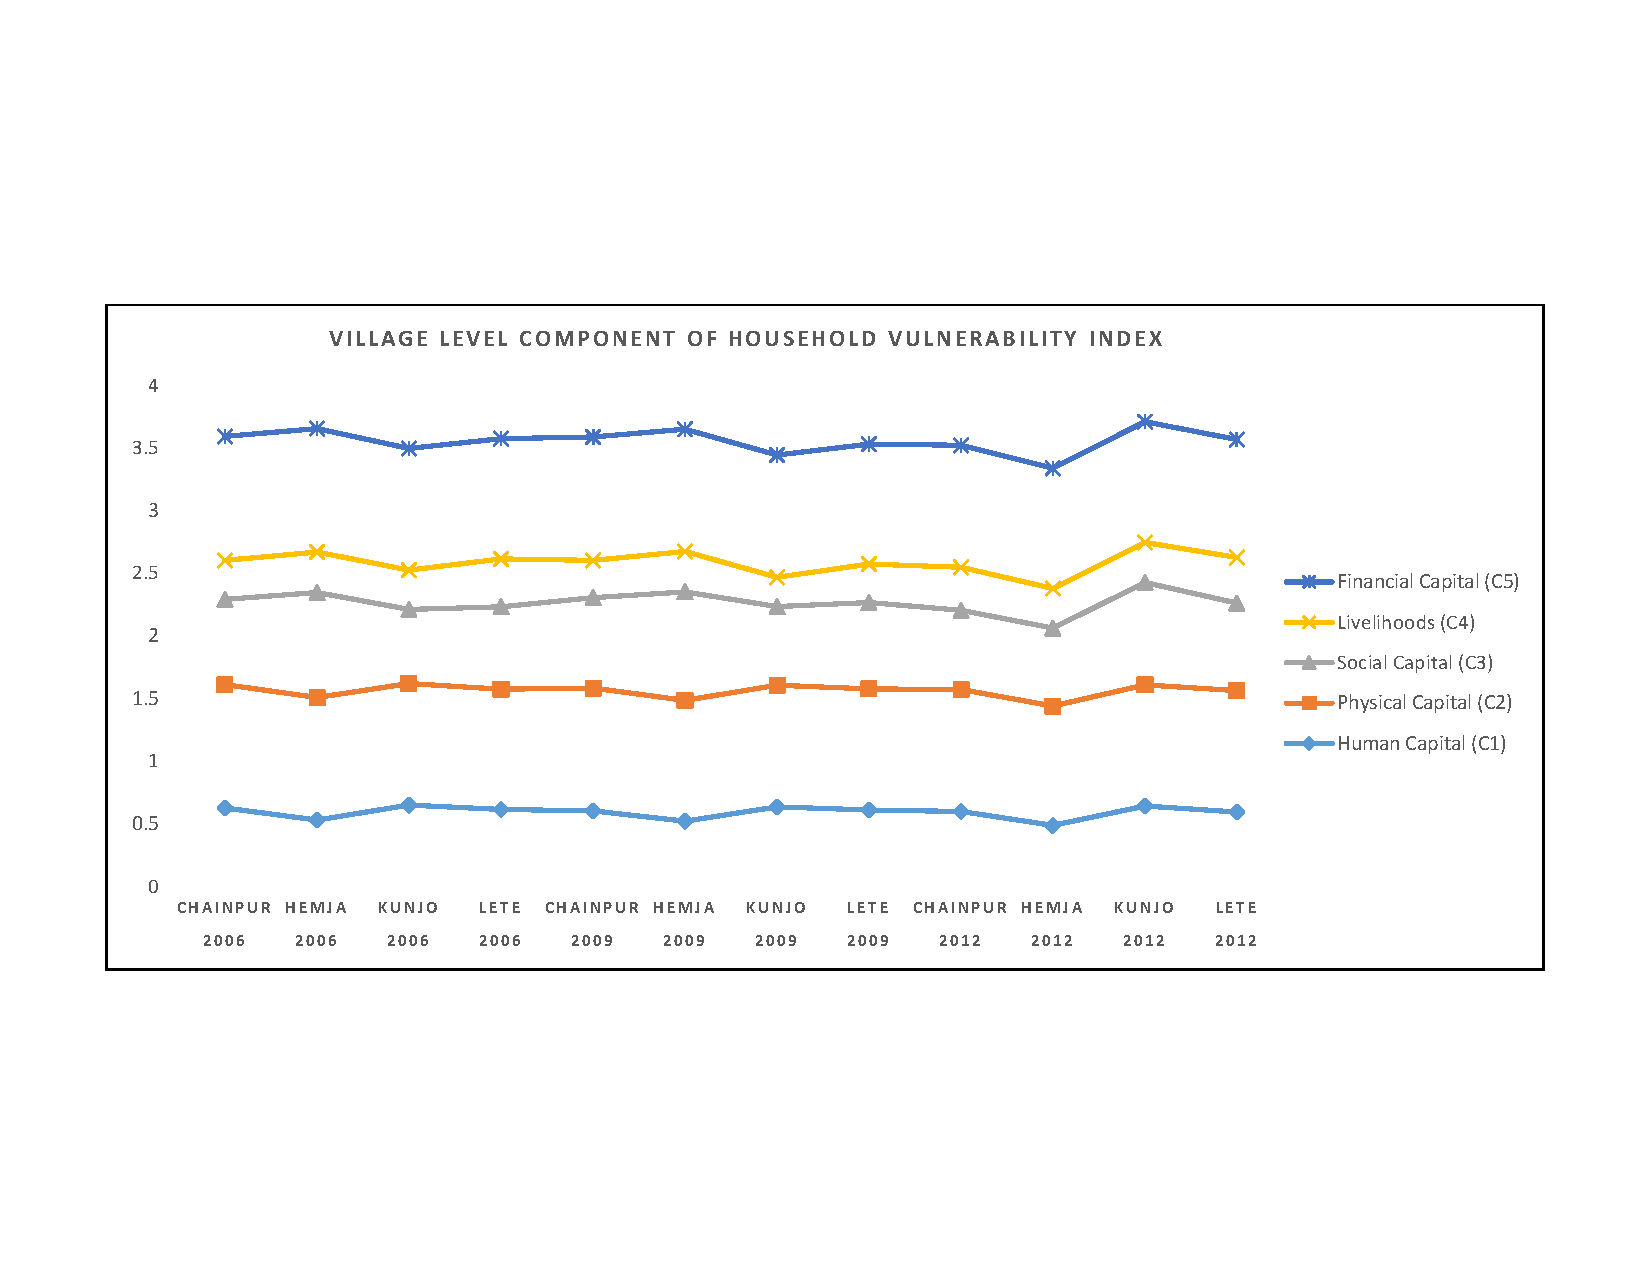
\includegraphics[scale=0.8]{HVI_Component_Village_Panel.pdf}
	\vspace{-50pt}
	\caption*{Appendix Fig 1: Village level HVI Components} 
	\label{fig:VDClevelhvicomponents}
	\captionsetup{skip=20pt}
\end{figure}
\end{landscape}

\begin{table}[ht] 
\captionsetup{labelformat=empty}
\caption*{Appendix Table 3 : Pooled OLS Regression} 
\label{} 
\renewcommand{\arraystretch}{1.1}
\resizebox{1.05\textwidth}{!}{%
	\begin{tabular}{@{\extracolsep{0.01pt}}lD{.}{.}{-3} D{.}{.}{-3} D{.}{.}{-3} D{.}{.}{-3} D{.}{.}{-3} D{.}{.}{-3} D{.}{.}{-3} } 
		\\[-1.6ex]\hline 
		\hline \\[-1.8ex] 
		& \multicolumn{7}{c}{\textit{Dependent variable:Household Vulnerability}} \\ 
		\cline{2-8} 		\\[-2.9ex] & \multicolumn{1}{c}{(1)} & \multicolumn{1}{c}{(2)} & \multicolumn{1}{c}{(3)} & \multicolumn{1}{c}{(4)} & \multicolumn{1}{c}{(5)} & \multicolumn{1}{c}{(6)} & \multicolumn{1}{c}{(7)}\\ 
		\hline \\[-1.8ex] 
		Env Dependence & 0.068^{***} & 0.068^{***} & 0.064^{***} & 0.062^{***} & 0.062^{***} & 0.049^{***} & 0.045^{***} \\ 
		& (0.012) & (0.012) & (0.012) & (0.012) & (0.012) & (0.012) & (0.012) \\ 
		& & & & & & & \\ 
		Debt &  & -0.001^{*} & -0.0004 & -0.0004 & -0.0004 & -0.0004 & -0.0005 \\ 
		&  & (0.0003) & (0.0003) & (0.0003) & (0.0003) & (0.0003) & (0.0003) \\ 
		& & & & & & & \\ 
		Depndency ratio &  &  & 0.022^{***} & 0.021^{***} & 0.021^{***} & 0.021^{***} & 0.020^{***} \\ 
		&  &  & (0.002) & (0.002) & (0.002) & (0.002) & (0.002) \\ 
		& & & & & & & \\ 
		Shock &  &  &  & 0.002^{*} & 0.002 & 0.001 & 0.001 \\ 
		&  &  &  & (0.001) & (0.001) & (0.001) & (0.001) \\ 
		& & & & & & & \\ 
		Constant & 0.557^{***} & 0.561^{***} & 0.550^{***} & 0.550^{***} & 0.552^{***} & 0.558^{***} & 0.562^{***} \\ 
		& (0.012) & (0.012) & (0.011) & (0.011) & (0.012) & (0.012) & (0.012) \\ 
		& & & & & & & \\ [-3.1ex]
		\hline \\[-2.5ex] 
		\textit{Fixed effects} & & & & & & & \\ 
		Year & \multicolumn{1}{c}{No} & \multicolumn{1}{c}{No} & \multicolumn{1}{c}{No} & \multicolumn{1}{c}{No} & \multicolumn{1}{c}{Yes} & \multicolumn{1}{c}{Yes} & \multicolumn{1}{c}{Yes} \\ 
		District & \multicolumn{1}{c}{No} & \multicolumn{1}{c}{No} & \multicolumn{1}{c}{No} & \multicolumn{1}{c}{No} & \multicolumn{1}{c}{No} & \multicolumn{1}{c}{Yes} & \multicolumn{1}{c}{Yes} \\ 
		VDC & \multicolumn{1}{c}{No} & \multicolumn{1}{c}{No} & \multicolumn{1}{c}{No} & \multicolumn{1}{c}{No} & \multicolumn{1}{c}{No} & \multicolumn{1}{c}{No} & \multicolumn{1}{c}{Yes} \\ 
		\hline \\[-2.5ex] 
		\textit{Fit statistics} & & & & & & & \\
		Observations & \multicolumn{1}{c}{1,284} & \multicolumn{1}{c}{1,284} & \multicolumn{1}{c}{1,284} & \multicolumn{1}{c}{1,284} & \multicolumn{1}{c}{1,284} & \multicolumn{1}{c}{1,284} & \multicolumn{1}{c}{1,284} \\ 
		R$^{2}$ & \multicolumn{1}{c}{0.024} & \multicolumn{1}{c}{0.027} & \multicolumn{1}{c}{0.105} & \multicolumn{1}{c}{0.107} & \multicolumn{1}{c}{0.108} & \multicolumn{1}{c}{0.126} & \multicolumn{1}{c}{0.131} \\ 
		Adjusted R$^{2}$ & \multicolumn{1}{c}{0.023} & \multicolumn{1}{c}{0.025} & \multicolumn{1}{c}{0.103} & \multicolumn{1}{c}{0.105} & \multicolumn{1}{c}{0.104} & \multicolumn{1}{c}{0.121} & \multicolumn{1}{c}{0.125} \\ 
		\hline 
		\hline \\[-1.8ex]  
	\end{tabular}
}
\textit{Note: Standard errors in the parenthesis} \hspace{2.52cm}{$^{*}$p$<$0.1; $^{**}$p$<$0.05; $^{***}$p$<$0.01} \\
\textit{Env. = Environmental}
\end{table} 
\begin{table}[H] 
\caption*{Appendix Table 4: Random Effects Regression} 
\label{}
\renewcommand{\arraystretch}{1.1}
\resizebox{1.05\textwidth}{!}{% 
	\begin{tabular}{@{\extracolsep{0.01pt}}lD{.}{.}{-3} D{.}{.}{-3} D{.}{.}{-3} D{.}{.}{-3} D{.}{.}{-3} D{.}{.}{-3} D{.}{.}{-3} } 
		\\[-1.8ex]\hline 
		\hline \\[-2.9ex] 
		& \multicolumn{7}{c}{\textit{Dependent variable:Household Vulnerability}} \\ 
		\cline{2-8} \\[-7ex] 
		& \\
		[-1.8ex] & \multicolumn{1}{c}{(1)} & \multicolumn{1}{c}{(2)} & \multicolumn{1}{c}{(3)} & \multicolumn{1}{c}{(4)} & \multicolumn{1}{c}{(5)} & \multicolumn{1}{c}{(6)} & \multicolumn{1}{c}{(7)}\\ 
		\hline \\[-3.9ex] 
		Env. Dependence & 0.035^{***} & 0.035^{***} & 0.037^{***} & 0.035^{***} & 0.034^{***} & 0.026^{**} & 0.024^{**} \\ [-1.5ex]
		& (0.011) & (0.011) & (0.011) & (0.011) & (0.011) & (0.011) & (0.011) \\ [-3.5ex]
		& & & & & & & \\ 
		Debt &  & -0.001^{*} & -0.0003 & -0.0004 & -0.0004 & -0.0004 & -0.0004 \\ [-1.5ex]
		&  & (0.0003) & (0.0003) & (0.0003) & (0.0003) & (0.0003) & (0.0003) \\ [-3.5ex]
		& & & & & & & \\ 
		Dependency ratio &  &  & 0.020^{***} & 0.019^{***} & 0.019^{***} & 0.019^{***} & 0.018^{***} \\[-1.5ex] 
		&  &  & (0.002) & (0.002) & (0.002) & (0.002) & (0.002) \\ [-3.5ex]
		& & & & & & & \\ 
		Shock &  &  &  & 0.002^{**} & 0.001 & 0.001 & 0.001 \\ [-1.5ex]
		&  &  &  & (0.001) & (0.001) & (0.001) & (0.001) \\ [-3.5ex]
		& & & & & & & \\ 
		Constant & 0.588^{***} & 0.592^{***} & 0.576^{***} & 0.576^{***} & 0.580^{***} & 0.581^{***} & 0.583^{***} \\ [-1.5ex] 
		& (0.011) & (0.011) & (0.011) & (0.011) & (0.011) & (0.011) & (0.011) \\ [-4.5ex]
		& & & & & & & \\ 
		\hline \\[-5ex] 
		\textit{Fixed effects} & & & & & & & \\  \\[-6ex]
		Year & \multicolumn{1}{c}{No} & \multicolumn{1}{c}{No} & \multicolumn{1}{c}{No} & \multicolumn{1}{c}{No} & \multicolumn{1}{c}{Yes} & \multicolumn{1}{c}{Yes} & \multicolumn{1}{c}{Yes} \\ [-1.5ex]
		District & \multicolumn{1}{c}{No} & \multicolumn{1}{c}{No} & \multicolumn{1}{c}{No} & \multicolumn{1}{c}{No} & \multicolumn{1}{c}{No} & \multicolumn{1}{c}{Yes} & \multicolumn{1}{c}{Yes} \\ [-1.5ex]
		VDC & \multicolumn{1}{c}{No} & \multicolumn{1}{c}{No} & \multicolumn{1}{c}{No} & \multicolumn{1}{c}{No} & \multicolumn{1}{c}{No} & \multicolumn{1}{c}{No} & \multicolumn{1}{c}{Yes} \\ 
		\hline \\[-5ex] 
		\textit{Fit statistics} & & & & & & & \\ [-1.5ex]
		Observations & \multicolumn{1}{c}{1,284} & \multicolumn{1}{c}{1,284} & \multicolumn{1}{c}{1,284} & \multicolumn{1}{c}{1,284} & \multicolumn{1}{c}{1,284} & \multicolumn{1}{c}{1,284} & \multicolumn{1}{c}{1,284} \\ [-1.5ex]
		R$^{2}$ & \multicolumn{1}{c}{0.007} & \multicolumn{1}{c}{0.010} & \multicolumn{1}{c}{0.072} & \multicolumn{1}{c}{0.075} & \multicolumn{1}{c}{0.076} & \multicolumn{1}{c}{0.091} & \multicolumn{1}{c}{0.095} \\ [-1.5ex]
		Adjusted R$^{2}$ & \multicolumn{1}{c}{0.007} & \multicolumn{1}{c}{0.008} & \multicolumn{1}{c}{0.070} & \multicolumn{1}{c}{0.072} & \multicolumn{1}{c}{0.072} & \multicolumn{1}{c}{0.085} & \multicolumn{1}{c}{0.089} \\ 
		\hline 
		\hline \\[-2.6ex]  
	\end{tabular} 
}
\textit{Note: Standard errors in the parenthesis} \hspace{2.52cm}{$^{*}$p$<$0.1; $^{**}$p$<$0.05; $^{***}$p$<$0.01} \\ [-1.83ex]
\textit{Env. = Environmental}
\end{table} 

\begin{table}[H] 
\caption*{Appendix Table 5: Fixed Effects Regression} 
\label{} 
\renewcommand{\arraystretch}{1.1}
\resizebox{1.05\textwidth}{!}{%
	\begin{tabular}{@{\extracolsep{5pt}}lD{.}{.}{-3} D{.}{.}{-3} D{.}{.}{-3} D{.}{.}{-3} D{.}{.}{-3} D{.}{.}{-3} D{.}{.}{-3} } 
		\\[-1.8ex]\hline 
		\hline \\[-3ex] 
		& \multicolumn{7}{c}{\textit{Dependent variable: Household Vulnerability}} \\ 
		\cline{2-8} 
		\\
		\\[-7.8ex] & \multicolumn{1}{c}{(1)} & \multicolumn{1}{c}{(2)} & \multicolumn{1}{c}{(3)} & \multicolumn{1}{c}{(4)} & \multicolumn{1}{c}{(5)} & \multicolumn{1}{c}{(6)} & \multicolumn{1}{c}{(7)}\\ 
		\hline \\[-3.98ex] 
		Env. Dependence & -0.003 & -0.003 & -0.001 & -0.001 & -0.004 & -0.004 & -0.004 \\ [-1.5ex]
		& (0.013) & (0.013) & (0.013) & (0.013) & (0.013) & (0.013) & (0.013) \\ [-3.5ex]
		& & & & & & & \\ 
		Debt &  & -0.0004 & -0.0003 & -0.0003 & -0.0003 & -0.0003 & -0.0003 \\ [-1.5ex]
		&  & (0.0004) & (0.0004) & (0.0004) & (0.0004) & (0.0004) & (0.0003) \\[-3.5ex] 
		& & & & & & & \\ 
		Dependency ratio &  &  & 0.015^{***} & 0.015^{***} & 0.014^{***} & 0.014^{***} & 0.014^{***} \\ [-1.5ex]
		&  &  & (0.003) & (0.003) & (0.003) & (0.003) & (0.002) \\ [-3.5ex]
		& & & & & & & \\ 
		Shock &  &  &  & 0.002^{*} & 0.001 & 0.001 & 0.001 \\ [-1.5ex]
		&  &  &  & (0.001) & (0.001) & (0.001) & (0.001) \\ [-4ex]
		& & & & & & & \\ \hline \\[-5ex] 
		\textit{Fixed Effexts} 	&  &  &  &  &  &  & \\ [-1.5ex]
		Year & \multicolumn{1}{c}{No} & \multicolumn{1}{c}{No} & \multicolumn{1}{c}{No} & \multicolumn{1}{c}{No} & \multicolumn{1}{c}{Yes} & \multicolumn{1}{c}{Yes} & \multicolumn{1}{c}{Yes} \\ [-1.5ex] 
		District & \multicolumn{1}{c}{No} & \multicolumn{1}{c}{No} & \multicolumn{1}{c}{No} & \multicolumn{1}{c}{No} & \multicolumn{1}{c}{No} & \multicolumn{1}{c}{Yes} & \multicolumn{1}{c}{Yes} \\ [-1.5ex]
		VDC & \multicolumn{1}{c}{No} & \multicolumn{1}{c}{No} & \multicolumn{1}{c}{No} & \multicolumn{1}{c}{No} & \multicolumn{1}{c}{No} & \multicolumn{1}{c}{No} & \multicolumn{1}{c}{Yes} \\ [-1.ex]
		\hline \\[-5ex] 
		\textit{Fit statistics} 	&  &  &  &  &  &  & \\ [-1.5ex]
		Observations & \multicolumn{1}{c}{1,284} & \multicolumn{1}{c}{1,284} & \multicolumn{1}{c}{1,284} & \multicolumn{1}{c}{1,284} & \multicolumn{1}{c}{1,284} & \multicolumn{1}{c}{1,284} & \multicolumn{1}{c}{1,284} \\ [-1.5ex]
		R$^{2}$ & \multicolumn{1}{c}{0.00005} & \multicolumn{1}{c}{0.002} & \multicolumn{1}{c}{0.034} & \multicolumn{1}{c}{0.037} & \multicolumn{1}{c}{0.042} & \multicolumn{1}{c}{0.042} & \multicolumn{1}{c}{0.042} \\ [-1.5ex]
		Adjusted R$^{2}$ & \multicolumn{1}{c}{-0.501} & \multicolumn{1}{c}{-0.500} & \multicolumn{1}{c}{-0.453} & \multicolumn{1}{c}{-0.450} & \multicolumn{1}{c}{-0.446} & \multicolumn{1}{c}{-0.446} & \multicolumn{1}{c}{-0.446} \\ [-0.5ex]
		\hline 
		\hline \\[-2.8ex] 
	\end{tabular} 
}
\textit{Note: Standard errors in the parenthesis} \hspace{2.52cm}{$^{*}$p$<$0.1; $^{**}$p$<$0.05; $^{***}$p$<$0.01} \\ [-1.83ex]
\textit{Env. = Environmental}
\end{table}
\clearpage
\begin{center}
\textbf{Appendix on Diagnostic Test Results}
\end{center}
\textbf{Appendix B1:
Lagrange Multiplier Test - (Honda) Time effects test}

data:  HVI $ \sim $ Environmental Dependency + Debt + Dependency ratio + Shock +  ...\\
\hspace{2cm}$normal = 10.822$, $p-value <2.2e-16$\\
\hspace{2cm}alternative hypothesis: significant effects\\

\textbf{Appendix B2:
F test for individual effects}

data:  HVI $ \sim $ Environmental Dependency + Debt + Dependency ratio + shock+...\\
$F = 2.4874$, $df1 = 427$, $df2 = 852$, $p-value < 2.2e-16$\\
alternative hypothesis: significant effects\\

\textbf{Appendix B3: Lagrange Multiplier Test - (Breusch-Pagan)}

data:  HVI $ \sim $ Environmental Dependency + Debt + Dependency ratio + shock+...\\
$chisq = 117.12$, $df = 1$, $p-value < 2.2e-16$\\
alternative hypothesis: significant effects\\

\textbf{Appendix B4: Hausman Test}
data:  HVI $ \sim $ Environmental Dependency + Debt + Dependency ratio + shock+...\\
$chisq = 25.48$, $df = 6$, $p-value = 0.0002782$\\
alternative hypothesis: one model is inconsistent\\
\end{document}